% TODO: Rename "thm" to "theorem" in labels.
% TODO: Put "label" at the beginning of sentences.
% TODO: Consider to use $\tilde$ instead of $\widetilde$ when it can be small.
\documentclass[candidate, subf, href, colorlinks]{disser}
% Add `fixint` for straight integral signs

\usepackage [T2A] {fontenc}
\usepackage [utf8] {inputenc}
\usepackage [russian, main = english] {babel}
\usepackage [autostyle] {csquotes}
\usepackage [intlimits] {amsmath}
\usepackage {amssymb}
\usepackage {amsfonts}
\usepackage {amsthm}
\usepackage {hyperref}
\usepackage {array}
\usepackage {multicol}
\usepackage {mathrsfs}
\usepackage {bm}
\usepackage {physics}
\usepackage {units}
\usepackage [symbol] {footmisc}
\usepackage {algorithm}
\usepackage {algorithmic}
\usepackage {caption}

% Margins
\usepackage[a4paper, mag=1000, left=2.5cm, right=1cm, top=2cm, bottom=2cm, headsep=0.7cm, footskip=1cm]{geometry}

\usepackage{wrapfig} % floating figures

% Previously used biblatex
% \usepackage[style=gost-numeric, backend=biber, language=auto, hyperref=auto, autolang=other, sorting=none] {biblatex}

% Biblatex usage same as for resume
\usepackage[
	bibstyle=gost-numeric,
	backend=biber,
	language=auto,
	hyperref=auto,
	autolang=other,
	defernumbers=true,
	movenames=false,
	sorting=none,
	maxbibnames=99
] {biblatex}

\addbibresource{bibliography.bib} % bibliography source

% Page number position config
\pagestyle{footcenter}
\chapterpagestyle{footcenter}

% Declarations
\newtheorem{proposition}{Proposition}
\newtheorem{corollary}{Corollary}
\newtheorem{lemma}{Lemma}
\newtheorem{definition}{Definition}
\newtheorem{remark}{Remark}
\newtheorem*{lemma*}{Lemma}
\newtheorem*{remark*}{Remark}
\newtheorem{theorem}{Theorem}
\newtheorem*{theorem*}{Theorem}
\newtheorem{hypothesis}{Hypothesis}
% TODO: Try to remove "thehypothesis" from the command below.
\renewcommand\thehypothesis{\Roman{hypothesis}}

\newenvironment{psm}
	{\left( \begin{smallmatrix}}
	{\end{smallmatrix} \right) }

\DeclareMathOperator*{\argmax}{arg\,max}
\newcommand{\sn}{\mathop\mathrm{sn}}
\newcommand{\cn}{\mathrm{cn}}
\newcommand{\dn}{\mathop\mathrm{dn}}
\newcommand{\cd}{\mathop\mathrm{cd}}

\renewcommand{\thefootnote}{\fnsymbol{footnote}}
\renewcommand\multicitedelim{\addcomma\space}

\captionsetup[algorithm]{
  labelfont = bf,
  labelsep = period
}

\begin{document}

\institution{Московский институт электронной техники (МИЭТ)}

% UDC number
\libcatnum{519.6}

\author{Лебедев Михаил Евгеньевич}

\topic{\dots}

\specnum{05.13.18}
\spec{Математическое моделирование, численные методы и комплексы программ}

\title{ДИССЕРТАЦИЯ \\ на соискание ученой степени \\ кандидата физико-математических наук}

\sa{Г. Л. Алфимов}
\sastatus{д.~ф.-м.~н., проф.}

\city{Москва}
\date{\number\year}


% Content
\tableofcontents

% Introduction
\chapter*{Itroduction}
\addcontentsline{toc}{chapter}{Introduction}

One dimensional Gross--Pitaevskii equation (describes ``cigar-shaped'' condensate) takes form:
\begin{equation}
	i \Psi_t + \Psi_{xx} + U(x) \Psi + P(x) |\Psi|^2 \Psi = 0.
\label{eq:gross-pitaevskii}
\end{equation}

Here $\Psi(t, x)$ is the macroscopic wave function of the condensate, $U(x)$ corresponds to the potential of the trap holding the condensate, and $P(x)$ describes characteristic length of the atomic interactions.
Function $P(x)$ is called as {\it pseudopotential} which is induced by spatial periodic modulation.
This can be achieved in BEC by means of the Feshbach resonance controlled by magnetic or optical field \cite{PollackDriesJunkerChenCorcovilosHulet, ChinGrimmJulienneTsienga, BauerLetterVoRempeDurr}.
In the nonlinear optics spatial modulation of the Kerr coefficient can be induced by inhomogeneous density of resonant nonlinearity-enhancing dopants implanted into the waveguide \cite{HukriedeRundeKip}.

\dots

% Why real? All definitions! Stationary states equation.
% Energy and norm for the general case (U(x), P(x)).
 

% Literature review
% \input{review}

% First chapter
% TODO: Labels in the beginning, not in the end.
\chapter{General Propositions on Regular and Singular Solutions for Stationary States Equation $u_{xx} + Q(x) u + P(x) u^3 = 0$}
\label{chapter:I}

\section{Objectives}

In this chapter we formulate general statements about singular and regular solutions for the equation
\begin{equation}
	u_{xx} + Q(x) u + P(x) u^3 = 0.
	\label{eq:main}
\end{equation}
% TODO: Move this part to the introduction.
%As it was shown previously this equation follows from the original Gross--Pitaevskii equation by the the substitution
%\begin{equation}
%	\Psi(t, x) = u(x) e^{-i \omega t},
%\end{equation}
%where the corresponding localization conditions allow us to consider $u(x)$ as a real-valued function.
In general, we suppose that $Q(x), P(x) \in C^1(\mathbb{R})$ and will impose additional restrictions further when it's needed.
% TODO: Definitions of "regular / singular solution" and "collapse" must be presented in introduction.
Mainly we address two questions: (A) when do exist regular solutions of \eqref{eq:main}; (B) what are the conditions for the functions $Q(x)$ and $P(x)$ which can guarantee the existence of the singular solutions for equation \eqref{eq:main}; and (C) what is the behaviour of the collapsing solutions near the collapse point.
In this chapter partial answer to the question (A) is given by the Proposition~\ref{prop:absense-of-singular-solutions}.
On other hand Propositions~\ref{prop:singular-families} and \ref{prop:all-solutions-are-singular} give a partial answer to the question (B).
In particular Proposition~\ref{prop:singular-families} states that if the function $P(x)$ is negative at a point $x = x_0$ then there exist two one-parametric families of solutions collapsing at $x_0$.
Proposition~\ref{prop:singular-families} determines an asymptotic behaviour of these singular solutions families, which gives an answer to the question (C) for these families.

\section{Non-existence of Singular Solutions: $P(x) \ge P_0 > 0$}

This section contains a sufficient condition for non-existence of singular solutions for equation \eqref{eq:main}.
It's given by the following proposition.

\begin{proposition}
	Let functions $Q(x), P(x) \in C^1(\mathbb{R})$, moreover:
	\begin{enumerate}
		\item[(a)] $P(x) \ge P_0 > 0$, $|P'(x)| \le \widetilde{P}$;
		\item[(b)] $Q(x) \ge Q_0$, $|Q'(x)| \le \widetilde{Q}$;
	\end{enumerate}
	then solution of the Cauchy problem for equation \eqref{eq:main} with arbitrary initial conditions $u(x_0) = u_0$, $u_{x}(x_0) = u_0'$ can be continued to the whole real axis $\mathbb{R}$.
	\label{prop:absense-of-singular-solutions}
\end{proposition}
\begin{proof}
	By the existence and uniqueness theorem for ODE there exists an interval $[x_0; x_1)$ such that the solution of the Cauchy problem $u(x)$ for equation \eqref{eq:main} with initial conditions $u(x_0) = u_0$, $u_{x}(x_0) = u_0'$ exists and is unique on this interval, and $u(x) \in C^2[x_0; x_1)$.
	Suppose that $[x_0; x_1)$ is the maximum interval for existence of $u(x)$.
	It means that solution of the Cauchy problem $u(x)$ cannot be continued beyond the point $x_1$.
	Multiplying the original equation by $4u_{x}(x)$ and integrating it over $[x_0, x)$, $x < x_1$, we have the following relation:
	\begin{equation}
	\begin{aligned}
		& 2 u_x^2(x)) + 2 Q(x) u^2(x) - 2 \int \limits_{x_0}^{x} Q'(\xi) u^2(\xi) d\xi + P(x) u^4(x) - \int \limits_{x_0}^x P'(\xi) u^4(\xi) d\xi = \\
		& \quad = 2 (u_0')^2 + 2 Q(x_0) u_0^2 + P(x_0) u_0^4 \equiv C.
		\label{eq:aux-04}
	\end{aligned}	
	\end{equation}
	Omit the term $u_{x}^2(x) \ge 0$ in the left-hand side of the equality, and take into account the lower limits for $Q(x)$, $P(x)$ given by conditions (a), (b).
	Then we arrive at the following inequality:
	\begin{equation}
		2 Q_0 u^2(x) + P_0 u^4(x) \le C + 2 \int \limits_{x_0}^{x} Q'(\xi) u^2(\xi) d\xi + \int \limits_{x_0}^{x} P'(\xi) u^4(\xi) d\xi.
	\end{equation}
	Replace the derivatives $Q'(\xi)$ and $P'(\xi)$ with their upper bounds: $Q'(\xi) \le \widetilde{Q}$, $P'(\xi) \le \widetilde{P}$, where $\widetilde{Q} \ge 0$, $\widetilde{P} \ge 0$.
	Multiplying both sides of the inequality by $P_0$, we have
	\begin{equation}
		2 Q_0 P_0 u^2(x) + P_0^2 u^4(x) \le P_0 C + 2 P_0 \widetilde{Q} \int \limits_{x_0}^{x} u^2(\xi) d\xi + P_0 \widetilde{P} \int \limits_{x_0}^{x} u^4(\xi) d\xi.
		\label{eq:aux-01}
	\end{equation}
	Let $v(x) = (P_0 u^2(x) + Q_0)^2$, $v(x) \ge 0$, substituting this into \eqref{eq:aux-01} gives
	\begin{equation}
		v(x) \le \widetilde{C} + \dfrac{\widetilde{P}}{P_0} \int \limits_{x_0}^{x} w(v(\xi)) d\xi.
		\label{eq:aux-02}
	\end{equation}
	Here $\widetilde{C} = P_0 C + Q_0^2 \ge 0$, $\alpha = 2 \widetilde{Q} P_0 / \widetilde{P} \ge 0$, and $w(v)$ is defined by
	\begin{equation}
		w(v) \equiv \alpha (\sqrt{v} - Q_0) + (\sqrt{v} - Q_0)^2.
	\end{equation}
	Consider the function
	\begin{equation}
		G(s) = \int \limits_{s_0}^{s} \dfrac{dv}{w(v)}.
	\end{equation}
	Here $s_0 > Q_0^2$ is an arbitrary constant, $s \ge s_0$.
	Since $w(v)$ is a positive and monotonically decreasing function, and the integral
	\begin{equation}
		\int \limits_{s_0}^{+\infty} \dfrac{dv}{w(v)}
	\end{equation}
	diverges, one can conclude that $G(s)$ is a positive, monotonically increasing, and unbounded function.
	It means that inverse function $G^{-1}(r)$ is well-defined for $r \ge 0$, increases monotonically, and is unbounded.
	The above-mentioned statements allow as to apply {\it Bihary} inequality \cite[theorem 2.3.1]{Pachpatte} to \eqref{eq:aux-02}.
	This results in the inequality
	\begin{equation}
		v(x) \le G^{-1} \left( G(\widetilde{C}) + \dfrac{\widetilde{P}}{P_0} \int \limits_{x_0}^{x} d\xi \right) = G^{-1} \left( G(\widetilde{C}) \dfrac{\widetilde{P}}{P_0} (x - x_0) \right) < \infty.
		\label{eq:bihari}
	\end{equation}
	Inequality \eqref{eq:bihari} is valid for all $x \in [x_0; x_1)$.
	It follows from \eqref{eq:bihari} that function $v(x)$ is bounded on the whole interval $[x_0; x_1)$:
	\begin{equation}
		v(x) \le M = G^{-1} \left( G(\widetilde{C}) + \dfrac{\widetilde{P}}{P_0} (x_1 - x_0) \right).
	\end{equation}
	We observe that $\widetilde{C} \ge Q_0^2$, moreover $\widetilde{C} = Q_0^2$ only if $u_0 = u_0' = 0$.
	It means that $G(s)$ is well-defined for each constant $\widetilde{C}$ corresponding to any non-zero solution $u(x)$.
	The boundedness of $v(x)$ yields that solution $u(x)$ is also bounded on the segment $[x_0; x_1)$:
	\begin{equation}
		|u(x)| \le \sqrt{\dfrac{\sqrt{M} - Q_0}{P_0}}, \quad x \in [x_0; x_1).
		\label{eq:aux-03}
	\end{equation}
	Substitution of \eqref{eq:aux-03} into \eqref{eq:aux-04} gives the upper bound for the derivative $u_{x}(x)$ on the interval $x \in [x_0; x_1)$.
	Since functions $u(x)$ and $u_{x}(x)$ are continuous and bounded on $[x_0; x_1)$, the values $u(x_1) = u_1$ and $u_{x}(x_1) = u_1'$ are finite.
	Hence there exists a continuation of the solution to the Cauchy problem with the initial conditions $u(x_0) = u_0$, $u_{x}(x_0) = u_0'$ on a larger interval beyond the initial $[x_0; x_1)$.
	It contradicts the original assumption.
	
	Thus we have proved that the solution can be continued for $x > x_0$.
	In order to prove the same statement for $x < x_0$, one can make a substitution $x \to -x$ and employ the same reasoning.
\end{proof}

\begin{corollary}
	If the conditions (a) and (b) are satisfied not on the whole real axis $\mathbb{R}$, but only on some interval $[x_1; x_2]$, then a solution of the Cauchy problem for equation \eqref{eq:main} with arbitrary initial conditions does not collapse at any point of the segment $[x_1; x_2]$.
\end{corollary}

\section{Asymptotic Behaviour at a Collapse Point: $P(x_0) < 0$}

\subsection{Asymptotic Expansions}

If $P(x)$ is negative at least at one point $x_0 \in \mathbb{R}$, formal asymptotic expansions predict existence of two one-parametric families of the solutions for the equation \eqref{eq:main} collapsing at this point.

Let us construct these asymptotic expansions.
We suppose that $P(x_0) = -1$ (this condition can be achieved by a simple renormalisation of the independent variable), denote $\eta = x - x_0$, and assume that in the vicinity of the point $x = x_0$, the following expansions are valid:
\begin{equation}
	Q(x) = Q_0 + Q_1 \eta + Q_2 \eta^2 \dots, \quad P(x) = -1 + P_1 \eta + P_2 \eta^2 + \dots.
\end{equation}
Substituting these expansions into \eqref{eq:main}, we have
\begin{equation}
	u_{\eta\eta} + (Q_0 + Q_1 \eta + Q_2 \eta^2 \dots)u + (-1 + P_1 \eta + P_2 \eta^2 + \dots) u^3 = 0.
	\label{eq:aux-11}
\end{equation}
If a solution $u(\eta)$ of equation \eqref{eq:aux-11} collapses at the point $\eta = 0$ then $u(\eta) \to \pm \infty$, when $\eta \to 0$.
Let $\eta$ approach zero {\it from the right}, $\eta > 0$.
The change $v(\eta) = \eta u(\eta)$, $\eta = e^{-t}$ gives
\begin{equation}
	v_{tt} + 3v_{t} + 2v + e^{-2t} Q(t) v + P(t) v^3 = 0.
	\label{eq:asymptotic-problem}
\end{equation}
Determine the main term of the expansion by balancing $2v$ and $-v^3$ terms.
We have
\begin{equation}
	V_0(t) = \pm \sqrt{2}.
	\label{eq:main-term}
\end{equation}
Now let's define the first order term $V_1(t)$, $v(t) = \pm \sqrt{2} + V_1(t) + o(V_1(t))$.
Substituting the last expression into \eqref{eq:asymptotic-problem}, taking into account the expansions for the functions $Q(t)$, $P(t)$, and omitting the terms of order higher than $e^{-t}$, we obtain
\begin{equation}
	V_{1, tt} + 3V_{1, t} - 4V_1 = \mp 2 \sqrt{2} e^{-t},
\end{equation}
that gives $V_1(t) = \pm \frac{\sqrt{2}}{3} e^{-t}$.
Second, third, and forth order terms $V_n$, $n = 2, 3, 4$, can be found in a similar manner.
For each term the corresponding equation takes form:
\begin{equation}
	V_{n, tt} + 3V_{n, t} - 4V_n = C_n e^{-nt}.
	\label{eq:high-order-terms-equation}
\end{equation}
For $n = 2, 3$ solutions of equation \eqref{eq:high-order-terms-equation} are of the form $V_n \sim e^{-nt}$.
However in the case $n = 4$ the exponent degree in the right hand side coincides with one of the roots of the characteristic polynomial for the differential operator in the left-hand side.
In this case solution of equation \eqref{eq:high-order-terms-equation} must be chosen in the form $Ce^{-4t} - A_3 t e^{-4t}$.
Here $C$ in an arbitrary constant, while $A_3$ can be determined uniquely from the coefficients of the series expansions for $Q(t)$, $P(t)$.
If constant $C$ is fixed, at the further steps of this procedure the corresponding equations are uniquely solvable.
One can note that switching of $+$ to $-$ in the expression \eqref{eq:main-term} leads to the corresponding change of signs for all coefficients $A_n$, $n = 0, 1,...$, that is natural due to the invariance of equation \eqref{eq:main} with respect to the change $u \to -u$.
We have
\begin{equation}
	\pm v(t) = \sqrt{2} + A_0 e^{-t} + A_1 e^{-2t} + A_2 e^{-3t} + A_3 \cdot (-t) \cdot e^{-4t} + C e^{-4t} + \dots.
	\label{eq:expansion-intermediate}
\end{equation}
Explicit expressions for $A_0, \dots, A_3$ are:
\begin{eqnarray}
	& A_0 & = \dfrac{\sqrt{2}}{3} P_1; \label{eq:aux-A0} \\
	& A_1 & = \dfrac{\sqrt{2}}{3} P_2 + \dfrac{\sqrt{2}}{6} Q_0 + \dfrac{2 \sqrt{2}}{9} P_1^2; \label{eq:aux-A1} \\
	& A_2 & = \frac{2\sqrt{2}} 3P_2 P_1 + \frac{7\sqrt{2}}{27} P_1^3 + \frac{\sqrt{2}} 6Q_0 P_1 + \frac{\sqrt{2}} 4Q_1 + \frac{\sqrt{2}} 2P_3; \label{eq:aux-A2} \\
	& A_3 & = -\dfrac{\sqrt{2}}{6} Q_1 P_1 - \dfrac{\sqrt{2}}{5} Q_2 - \dfrac{32 \sqrt{2}}{45} P_2 P_1^2 - \dfrac{3 \sqrt{2}}{5} P_3 P_1 - \\
	&& - \dfrac{2 \sqrt{2}}{15} P_2 Q_0 -\dfrac{2 \sqrt{2}}{15} Q_0 P_1^2 - \dfrac{2 \sqrt{2}}{5} P_4 - \dfrac{28 \sqrt{2}}{135} P_1^4 - \dfrac{4 \sqrt{2}}{15} P_2^2. \label{eq:aux-A3}
\end{eqnarray}

In the other case when $\eta \to 0$ {\it from the left}, $\eta < 0$, similar expansions can be constructed by mean of changes of variables $v(\eta) = \eta u(\eta)$, $\eta = -e^{-t}$.
Expressions for the coefficient $A_n$ remain the same as for $\eta > 0$.

Finally we get an asymptotic expansion for the original solution $u(x)$ for $x \to x_0 \pm 0$:
\begin{equation}
	\pm u(x) = \dfrac{\sqrt{2}}{\eta} + A_0 + A_1 \eta + A_2 \eta^2 + A_3 \eta^3 \ln |\eta| + C \eta^3+ A_4 \eta^4 \ln |\eta| + \dots.
	\label{eq:expansion}
\end{equation}
Here $\eta = x - x_0$, $A_0, \dots, A_3$ are determined by equations \eqref{eq:aux-A0}-\eqref{eq:aux-A3}, and all other coefficients $A_n$, $n > 3$ can be expressed through $Q_n$, $P_n$ and arbitrary constant $C$.

Summarizing all the above mentioned, one can say that asymptotic expansion \eqref{eq:expansion} {\it predicts the existence} of two one-parametric families of solutions collapsing at the point $x_0$.
These families are connected by the symmetry $u \to -u$.
When $x \to x_0$, the solutions from one of these families tend to $+\infty$, while the solutions from another family tend to $-\infty$ correspondingly.

\subsection{Existence of One-Parametric Families of Collapsing Solutions}

Strictly speaking, formal asymptotic expansions \eqref{eq:expansion} do not imply the existence of one-parametric families of solutions collapsing at point $x_0$.
However, the following rigorous statement holds.

\begin{proposition}
	Let $\Omega$ be a neighbourhood of the point $x_0$, $Q(x) \in C^2(\Omega)$ and $P(x) \in C^4(\Omega)$.
	Then there exist two $C^1$-smooth one-parametric families of solutions for equation \eqref{eq:main} corresponding to expansions \eqref{eq:expansion}, collapsing at the point $x = x_0$ (while approaching from the left, $x < x_0$), and connected by a symmetry $u \to -u$.
	Each of these families can be parametrized by a free variable $C \in \mathbb{R}$ from the expansions \eqref{eq:expansion}.
\label{prop:singular-families}
\end{proposition}
\begin{proof}
	Due to the condition of proposition the following expansions are valid:
	\begin{eqnarray}
		& Q(x) & = Q_0 + Q_1 \eta + Q_2 \eta^2 + \widetilde{Q}(\eta) \eta^3; \\
		& P(x) & = -1 + P_1 \eta + P_2 \eta^2 + P_3 \eta^3 + P_4 \eta^4 + \widetilde{P}(\eta) \eta^5.
	\end{eqnarray}
	Here $\eta = x - x_0$, and $\widetilde{Q}, \widetilde{P} \in C(\Omega)$.
	To prove existence of the family that corresponds to the $+$ sign in \eqref{eq:expansion}	 we introduce the function $z(\eta)$ as follows:
	\begin{equation}
		u(x) = \dfrac{\sqrt{2}}{\eta} + A_0 + A_1 \eta + A_2 \eta^2 + A_3 \eta^3 \ln(-\eta) + z(\eta) \eta^3,
		\label{eq:aux-20}
	\end{equation}
	($z(\eta)$ is a new unknown function).
	Coefficients $A_0, \dots, A_3$ are chosen accordingly to the expressions \eqref{eq:aux-A0}-\eqref{eq:aux-A3}, so the coefficients at the terms $\eta^{-2}$, $\eta^{-1}$, $\eta^0$, and $\eta$ vanish.
	It's easy to check that direct substitution of the \eqref{eq:aux-20} into \eqref{eq:main} yields
	\begin{equation}
		z_{\eta\eta} + \dfrac{6}{\eta} z_{\eta} + g(\eta, z) = 0,
		\label{eq:aux-z}
	\end{equation}
	where $g(\eta, z)$ is a third order polynomial with respect to $z$, and $g(\eta, z) \sim \frac{\ln(-\eta)}{\eta}$ when $\eta \to -0$ and $z$ is fixed.
	The change of variable $\eta = -e^{-t}$ maps the point $\eta = 0$ into $t = +\infty$, and transforms equation \eqref{eq:aux-z} into
	\begin{equation}
		z_{tt} - 5z_t - f(t, z) = 0.
		\label{eq:aux-zt}
	\end{equation}
	Here $f(t, z) \sim t e^{-t}$ while $t \to +\infty$.
	Properties of the function $f(t, z)$ allows us to apply {\it Lemma on Bounded Solutions} from Appendix \ref{appendix:lemma-on-bounded-solutions} to equation \eqref{eq:aux-zt}.
	This lemma states that for $t \to +\infty$ all bounded solutions of equation \eqref{eq:aux-zt} tend to some constant $C$ when $t \to +\infty$, moreover for each $C \in \mathbb{R}$ there exists a unique solution that approaches to that constant asymptotically while $t \to +\infty$.
	Furthermore these solutions form a $C^1$-smooth family.
	Finally, we can return to previous equation \eqref{eq:aux-z}, and then to \eqref{eq:main} to get the initial statement of the proposition.
	The existence of the second family of solutions corresponding to the sign ``$-$'' in \eqref{eq:expansion} follows from the invariance of equation \eqref{eq:main} under the symmetry $u \to -u$.
\end{proof}

Similar one-parametric families of collapsing solutions exist from the right side of the point $x = x_0$.
The corresponding proof can be performed in the same way.

\section{All Solutions Are Singular: $P(x) \le P_0 < 0$, $Q(x) \le Q_0 < 0$}

It turns out that under some assumptions all non-trivial solutions of the equation \eqref{eq:main} are singular.
\begin{proposition}
\label{prop:all-solutions-are-singular}
	Let for $x \in \mathbb{R}$ the conditions $P(x) \le P_0 < 0$, $Q(x) \le Q_0 < 0$ take place.
	Then all solutions of equation \eqref{eq:main} are singular except for the zero one.
\end{proposition}

To prove this proposition we prove the following auxiliary lemma first.
\begin{lemma}
	Let $p, q > 0$ are real constants, then all solutions of equation
	\begin{equation}
		v_{xx} - q v - p v^3 = 0,
		\label{eq:aux-lemma}
	\end{equation}
	are singular except for the zero one.
\end{lemma}
\begin{proof}
	The solution of the Cauchy problem for equation \eqref{eq:aux-lemma} with initial conditions $v(x_0) = v_0$, $v_x(x_0) = v_0'$ can be written in an implicit form as follows:
	\begin{equation}
		\pm \int \limits_{v_0}^{v} \dfrac{d\xi}{\sqrt{C + q \xi^2 + \dfrac{p}{2} \xi^4}} = x - x_0;	\quad C \equiv (v_0')^2 - q v_0^2 - \dfrac{p}{2} v_0^4.
		\label{eq:aux-21}
	\end{equation}
	Choice of the sign in the left hand-side depends on the initial conditions and the value of $x$.
	Integral in the left hand-side of the equality \eqref{eq:aux-21} converges when $v \to \infty$, and hence there exist a value $x^*$,
	\begin{equation}
		x^* = x_0 \int \limits_{v_0}^{\infty} \dfrac{d\xi}{\sqrt{C + q \xi^2 + \dfrac{p}{2} \xi^4}},
	\end{equation}
	such that $v(x)$ goes to infinity while $x$ approaches to the $x^*$ 
	So a solution $v(x)$ with arbitrary non-zero initial conditions is singular, lemma is proved.
\end{proof}

Now we can prove the Proposition 3.
\begin{proof}[Proof of the Proposition 3.]
	We use a so-called {\it Comparison Lemma} from \cite[Appendix C]{AlfimovZezyulin}.
	Consider the equation
	\begin{equation}
		v_{xx} + Q_0 v + P_0 v^3 = 0.
	\end{equation}
	We introduce the notations
	\begin{eqnarray}
		& g(x, \xi) & = -Q(x) \xi - P(x) \xi^3; \\
		& f(x, \xi) = f(\xi) & = -Q_0 \xi - P_0 \xi^3.
	\end{eqnarray}
	Now we apply Comparison Lemma to the following pair of equations:
	\begin{eqnarray}
		&& u_{xx} = g(x, u) \label{eq:comparison-u}; \\
		&& v_{xx} = f(x, v) \label{eq:comparison-v}.
	\end{eqnarray}
	In the domain $D_+ = \{ x \in \mathbb{R}, \xi \in (0; +\infty) \}$ we have $f(x, \xi) \le g(x, \xi)$.
	Let $\widetilde{u}(x)$ be a solution of the Cauchy problem for equation \eqref{eq:comparison-u} with initial conditions $u(x_0) = u_0$, $u_x(x_0) = u_0'$.
	Chose the initial conditions for the Cauchy problem for equation \eqref{eq:comparison-v} as follows: $v(x_0) = u(x_0) = u_0$, $v_x(x_0) = u_x(x_0) = u_0'$; let $\widetilde{v}(x)$ be a solution for that problem.
	Let $u_0 > 0$, then one of the two cases takes place.
	\begin{enumerate}
		\item[(i)] $u_0' \ge 0$.
		Function $\widetilde{v}(x)$ increases monotonically; this fact can be easily established from the phase portrait of equation \eqref{eq:comparison-v}.
		Solution $\widetilde{u}(x)$ bounds the solution $\widetilde{v}(x)$ from above.
		But $\widetilde{v}(x)$ is singular.
		Then it follows from Comparison Lemma that solution $\widetilde{u}(x)$ is also singular.
		\item[(ii)] $u_0' < 0$.
		We make a change of variable $\widetilde{x} = -x$.
		In that case solution $\widetilde{v}(\widetilde{x})$ also increases monotonically, and since $\widetilde{u}(\widetilde{x})$ limits $\widetilde{v}(\widetilde{x})$ from above, $\widetilde{u}(\widetilde{x})$ is singular by Comparison Lemma, hence $\widetilde{u}(x)$ is also singular.
	\end{enumerate}
	Similarly in the domain $D_- = \{ x \in \mathbb{R}, \xi \in (-\infty; 0) \}$, the inequality $f(x, \xi) \ge g(x, \xi)$ holds.
	One can prove in the same manner that in the domain $D_-$ solution $u(x)$ is also singular.
\end{proof}

\section{Summary}

Our main findings on regular and singular solutions for the stationary states equation \eqref{eq:main} are summarised in Table \ref{tab:first-chapter-results}.
Our further findings are focused on the case when $P(x)$ changes its sign.
In the next chapter we describe a so-called {\it method of excluding of singular solutions} which allows us to classify all regular solutions of equation \eqref{eq:main} within the symbolic dynamics framework.

\begin{table}[h!]
	\centering
	\begin{tabular}{ | p{4cm} | l || p{10cm} | }
		\hline
		$P(x)$ & $Q(x)$ & \\
		\hline
		$P(x) > 0$ & --- & All the solutions can be continued to the whole real line, singular solutions do not exist (Proposition~\ref{prop:absense-of-singular-solutions}). \\
		\hline
		$P(x) < 0$ at least at one point $x = x_0$ & --- & There exists a pair of one-parametrical families of solutions collapsing at point $x = x_0$ and related by the symmetry $u \to -u$ (Proposition~\ref{prop:singular-families}). \\
		\hline
		$P(x) < 0$ & $Q(x) < 0$ & All solutions are singular except for the zero one (Proposition~\ref{prop:all-solutions-are-singular}). \\
		\hline
		$P(x)$ changes sign along $\mathbb{R}$ & --- & Singular solutions are generic.
		That fact allows to apply the so-called {\it method of excluding of singular solutions} and classify all regular solutions in terms of symbolic dynamics.
		We describe this method and its application in Chapter~\ref{chapter:II}. \\
		\hline
	\end{tabular}
	\caption{
		Summary of the results for the Chapter 1.
		The results of this Chapter were published in \cite{AlfimovLebedev}.
	}
	\label{tab:first-chapter-results}
\end{table}


% Second chapter
\chapter{Stationary states classification within symbolic dynamics framework}

\section{Objections}

In this chapter we describe an approach that is used further in order to classify all stationary state of one-dimensional GPE that are described by the stationary states equation:
\begin{equation}
	u_{xx} + Q(x) u + P(x) u^3 = 0.
	\label{eq:stationary}
\end{equation}
Here and after we assume $Q(x)$, $P(x)$ to be periodic functions of the same period $L$: $Q(x + L) = Q(x)$, $P(x + L) = P(x)$ which is quite typical for different physical applications.
We also assume functions $Q(x)$, $P(x)$ to be at least piece-wise continuously differentiable.
That allows us to split the whole real axis $\mathbb{R}$ into separate intervals where the corresponding Cauchy problem correctly defined and a solution for any initial conditions exists and is unique within each such interval.

Our classification approach is based on the technique proposed in the work \cite{AlfimovAvramenko}.
In \cite{AlfimovAvramenko} authors show that presence of a large number of singular solutions families allows to classify all remaining bounded solutions within a symbolic dynamics framework.
That leads us to another important requirement, function $P(x)$ must {\it changes its sign along the period} $L$.
As we saw in the previous chapter such fact guarantees the existence of singular solution families that in its turn becomes a foundation of the technique and makes the announced approach even possible.

Goal of this chapter is to provide a stationary states classification framework and point out the boundaries of its application.
Core idea is the following.
We define a Poincar\'e map $\mathcal{P}$ for the stationary states equation \eqref{eq:stationary}.
Since function $P(x)$ alternates its sing, Poincar\'e map $\mathcal{P}$ and an inverse map $\mathcal{P}^{-1}$ cannot be defined on the whole phase plane, instead they are defined on some phase plane subset.
Studying the domains of maps $\mathcal{P}$, $\mathcal{P}^{-1}$ is a crucial aspect of the proposed approach.
We determine conditions which allow to conclude that Poincar\'e map acts on the defined set as a kind of the {\it horseshoe map} \cite[Chapter 5]{GuekenheimerHolmes}.
Domains of the higher order maps $\mathcal{P}^2,~\mathcal{P}^3, \dots$ and domains of the inverse maps $\mathcal{P}^{-2},~\mathcal{P}^{-3}, \dots$ can be obtained by the refinement of the initial area.
Finally if some conditions are met and we can conclude that there exists one-to-one correspondence between all bounded solution of the equation \eqref{eq:stationary} and a points set on the phase plane which is a result of the above mentioned refinement.
That is what we call singular solution elimination method.

The presence of the horseshoe map structure allows us for each bounded solution uniquely specify a bi-infinite symbolic sequence over some alphabet (finite or even infinite) and such correspondence is also bijective.
We refer to the result bi-infinite sequence as {\it solution code} and the overall process as {\it solutions coding}.
Such coding, if possible, provides a complete picture of the bounded solutions family for the equation \eqref{eq:stationary} that can be highly demanded in different physical applications which involves Gross-Pitaevskii equation with both periodic potential and periodic pseudopotential.

\section{Geometry of the Poincar\'e map}

First of all let's introduce several definition which define basic structures and their relationships which are in the core of the overall further narration.

\subsection{Poincar\'e map}

Since we consider functions $Q(x)$, $P(x)$ to be $L$-periodic, let's introduce the Poincar\'e map associated with the period $L$.
Define the Poincar\'e map $\mathcal{P}: \mathbb{R}^2 \to \mathbb{R}^2$ in the following manner:
\begin{equation}
	\mathcal{P} \begin{pmatrix} u_0 \\ u_0' \end{pmatrix}
	= \begin{pmatrix} u_L \\ u_L' \end{pmatrix},
\end{equation}
where $u_L = u(L)$, $u_L' = u'(L)$, and $u(x)$ is a solution of the equation \eqref{eq:stationary} with initial conditions $u(0) = u_0$, $u'(0) = u_0'$.
Poincar\'e map by itself is an {\it area-preserving diffeomorphism}.
Obviously, and as we mentioned above, Poincar\'e map $\mathcal{P}$ and its inverse $\mathcal{P}^{-1}$ may not be defined on the whole phase plane $(u, u')$ of initial conditions.
Denote by $\mathscr{U}_L^+$ the domain of the map $\mathcal{P}$, and denote by $\mathscr{U}_L^-$ the domain of the map $\mathcal{P}^{-1}$ correspondingly.
Also define a set $\mathscr{U}_L$ as an intersection of the two above mentioned sets: $\mathscr{U}_L = \mathscr{U}_L^+ \cap \mathscr{U}_L^-$.

It's highly desired, and we'll require it further, that the defined set $\mathscr{U}_L$, produced by the Poincar\'e map $\mathcal{P}$, represents a so-called {\it island set} \cite{AlfimovAvramenko}.
Looking ahead, such set clearly reveals the horseshoe structure and allows us to formulate and prove all the essential theorems. 

\subsection{Island set}

\begin{definition}
	Let $\gamma > 0$ is fixed.
	A continuous function $f(x): \Delta \to \mathbb{R}^2$, $\Delta = [a, b]$ is called $\bm{\gamma}$-{\bf Lipschitz} function if $\forall x_1, x_2 \in \Delta$ the following inequality holds:
	\begin{equation}
		|f(x_1) - f(x_2)| \le \gamma |x_1 - x_2|.
	\end{equation}
\end{definition}

\begin{definition}
	We call {\bf island} an open curvilinear quadrangle $D \subset \mathbb{R}^2$ on the phase plane $(u, u')$ formed by two pairs of nonintersecting monotonic curves $\alpha^{\pm}$, $\beta^{\pm}$, moreover:
	\begin{itemize}
		\item curves $\alpha^{\pm}$ are graphs of monotonic $\gamma$-Lipschitz functions $u' = h_{\pm}(u)$, and a solution of the equation \eqref{eq:stationary} with initial conditions $(u_0, u_0') \in \alpha^{\pm}$ collapses at the point $x = -L$;
		\item curves $\beta^{\pm}$ are graphs of monotonic $\gamma$-Lipschitz functions $u = v_{\pm}(u')$, and a solution of the equation \eqref{eq:stationary} with initial conditions $(u_0, u_0') \in \beta^{\pm}$ collapses at the point $x = +L$;
		\item if the functions $h_{\pm}(u)$ are increasing then $v_{\pm}(u')$ are decreasing, and vice versa, if functions $h_{\pm}(u)$ are decreasing then $v_{\pm}(u')$ are increasing respectively.
	\end{itemize}	
\end{definition}

\begin{remark}
	For convenience hereinafter by monotonically increasing / decreasing function we mean a function that satisfy non-strict inequalities.
	We call function $f(x)$ monotonically increasing if for $x_1 < x_2$, $f(x_1) \le f(x_2)$, and monotonically decreasing if $f(x_1) \ge f(x_2)$.
\end{remark}

To emphasise the fact that Lipschitz constant $\gamma$ must be predefined we also refer to the island as \bm{$\gamma$}-{\bf island}.

\begin{remark}
	If $D$ is a $\gamma_1$-island and $\gamma_2 > \gamma_1$	then $D$ also is a $\gamma_2$-island.
\end{remark}

In our definition of island we explicitly specify its connection with initial equation \eqref{eq:stationary} and collapses of its solutions.
Further we'll see that such connection naturally comes from the dynamics of the $\mathcal{P}$ map for equation of such type.

\begin{remark}
	Solution of the Cauchy problem for the initial conditions at the  intersections of the $\alpha^{\pm}$, $\beta^{\pm}$ curves collapse both in $x = +L$ and $x = -L$ points.
\end{remark}

\begin{definition}
	Let $S$ be a finite or a countable set of indices.
	Define {\bf island set} as a set $\mathcal{D} = \bigcup_{i \in S} D_i$ that represents finite or countable union of disjoint islands.
\end{definition}

\begin{figure}[h]
\centering
	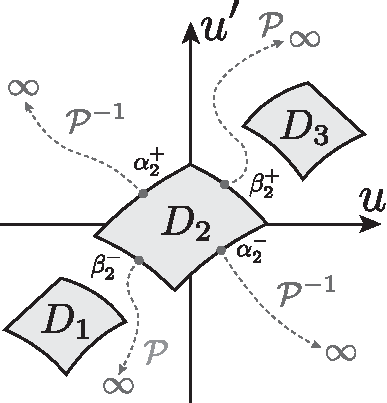
\includegraphics[scale = 1]{pic/islands set}
	\caption{Hypothetical example of an island set $\mathcal{D} = \bigcup_{i \in \{1, 2, 3\}} D_i$ on a plane of initial conditions for the equation \eqref{eq:stationary}. Boundaries of each component are mapped to the infinity by the $\mathcal{P}$ and $\mathcal{P}^{-1}$ maps (solution of the corresponding Cauchy problem is collapses).}
\label{fig:islands-set}
\end{figure}

\subsection{Curves and strips}

Move on to the definition of h,v-curves and h,v-strips.
Such curves and strips along with theirs transformations are the object of our attentive study.

\begin{definition}
	Let $D$ be an island bounded by curves $\alpha^{\pm}$, $\beta^{\pm}$.
	Consider a curve $\alpha$ that connects the opposite sides $\beta^{\pm}$ of the island $D$. 
	We call such curve {\bf h-curve} if it represents a graph of a monotonic $\gamma$-Lipschitz function $u' = h(u)$ and its monotonicity type coincide with the functions $u' = h_{\pm}(u)$ that correspond to the $\alpha^{\pm}$ boundaries of the island $D$.
	We also call {\bf h-strip} an open subset of the island $D$ bounded by two \emph{h}-curves.
\end{definition}

\begin{definition}
	Similarly consider a curve $\beta$ that connects opposite sides $\alpha^{\pm}$ of an island $D$.
	We call it {\bf v-curve} if it represents a graph of a monotonic $\gamma$-Lipschitz function $u = v(u')$ and its monotonicity type coincide with the functions $u = v_{\pm}(u')$ that correspond to the $\beta^{\pm}$ boundaries of the island $D$.
	In a like manner we call {\bf v-strip} an open subset of the island $D$ bounded by two \emph{v}-curves.
\end{definition}

\begin{remark}
	Island by itself represents a limit case of the h and v strips simultaneously.
\end{remark}

% TODO: make this figure a bit smaller
\begin{figure}[h]
\centering
	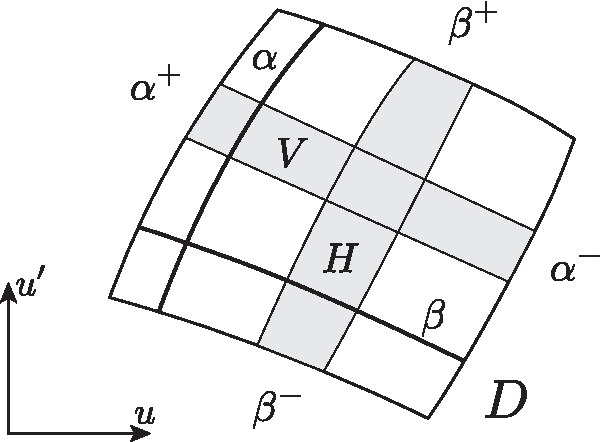
\includegraphics[scale = 1]{pic/curves and strips}
	\caption{An islands $D$ bounded by curves $\alpha^{\pm}$, $\beta^{\pm}$; h-curve $\alpha$, v-curve $\beta$, and two strips: h-strip $H$ and v-strip $V$.}
\label{fig:curves-and-strips}
\end{figure}

All above introduced definitions are illustrated on the figures \ref{fig:islands-set} and \ref{fig:curves-and-strips}.
At last let's define one additional property of island set along with $\mathcal{P}$, $\mathcal{P}^{-1}$ maps.

\begin{definition}
	Let $\mathcal{D}$ be an island set formed by the domains of the $\mathcal{P}$ and $\mathcal{P}^{-1}$ maps that act on this set.
	Consider two islands $D_1, D_2 \in \mathcal{D}$.
	We call the island $D_2$ {\bf forward-reachable} from the island $D_1$ if for any \emph{h}-curve $\alpha \in D_1$ with endpoints lying on the opposite boundaries $\beta_1^{\pm}$ of the island $D_1$ the intersection $\mathcal{P}(\alpha) \cap D_2$ is not empty.
	On the other hand we call the island $D_2$ {\bf backward-reachable} from the island $D_1$ if for any \emph{v}-curve $\beta \in D_1$ with endpoints lying on the opposite boundaries $\alpha_1^{\pm}$ of the island $D_1$ the intersection $\mathcal{P}^{-1}(\beta) \cap D_2$ is not empty.
	Finally we call the island $D_2$ {\bf reachable} from the $D_1$ if it satisfies both forward and backward reachability.
\end{definition}

\begin{remark}
	If an island $D_2$ is forward-reachable from $D_1$ then $D_1$ is backward-reachable from $D_2$ and vice versa.
\end{remark}

\begin{definition}
	We call an island set $\mathcal{D} = \bigcup_{i \in S} D_i$ {\bf complete} if for any $i, j$ island $D_i$ is reachable from $D_j$.
\end{definition}

\subsection{Thickness of strips}

Next we'll also need a definition of the strips thickness.
Let an h-strip $H$ lies inside an island $D$ and is bounded by h-curves $\alpha^+$ and $\alpha^-$.
Consider graphs of that curves as a functions of $u$: $u' = h_{\pm}(u)$.
By the definition $h_{\pm}(u)$ are $\gamma$-Lipschitz function.
Denote by $\Delta^{\pm}$ their domains.
Obviously due to the geometric properties of an island domains $\Delta^{\pm}$ do not coincide except the case when the opposite boundaries $\beta^{\pm}$ lying on the corresponding boundaries of the island $D$ are vertical straight lines.
Let $\Delta^+ = [u_0^+; u_1^+]$, $\Delta^- = [u_0^-; u_1^-]$, consider new domain $\Delta = \Delta^+ \cap \Delta^-$ and define functions $\widetilde{h}_{\pm}(u)$ on the new domain $\Delta$ as follows:
\begin{equation}
	\widetilde{h}_{\pm}(u) = \begin{cases}
		h_{\pm}(u_0^{\pm}) & u < u_0^{\pm}; \\
		h_{\pm}(u) & u \in \Delta^{\pm}; \\
		h_{\pm}(u_1^{\pm}) & u > u_1^{\pm}.
	\end{cases}
\label{eq:continuation}
\end{equation}
Since $h_{\pm}$ are $\gamma$-Lipschitz functions the new functions $\widetilde{h}_{\pm}$ are also $\gamma$-Lipschitz on the whole domain $\Delta$.
Denote by $\widetilde{\alpha}^{\pm}$ the resulted curves formed by the graphs $\widetilde{h}_{\pm}(u)$.

\begin{definition}
	By the {\bf thickness} of an h-strip $H$, denoted $d_\emph{h}(H)$, we mean the distance between curves $\widetilde{\alpha}^{\pm}$ in C-norm, i.e.
	\begin{equation}
		d_\emph{h}(H) = d(\widetilde{\alpha}^+, \widetilde{\alpha}^-) = \max \limits_{u \in \Delta} |\widetilde{h}_+(u) - \widetilde{h}_-(u)|.
	\label{eq:h-thickness}
	\end{equation}
\end{definition}

\begin{remark}
	For two \emph{h}-strips $H_1$, $H_2$ the following statement is valid: $H_2 \subseteq H_1 \Rightarrow \Delta_2 \subseteq \Delta_1$ and $d_\emph{h}(H_2) \le d_\emph{h}(H_1)$.
\end{remark}

\begin{definition}
	Let maximum of the expression \eqref{eq:h-thickness} is reached at a point $u_*$, i.e.
	\begin{equation}
		u_* = \argmax \limits_{u \in \Delta} |\widetilde{h}_+(u) - \widetilde{h}_-(u)|.
	\label{eq:argmax}
	\end{equation}
	We call an \emph{h}-strip $H$ {\bf well-measurable} if $u_* \in \Delta^+ \cap \Delta^-$.
\label{def:well-measurable}
\end{definition}

\begin{figure}[h]
\centering
	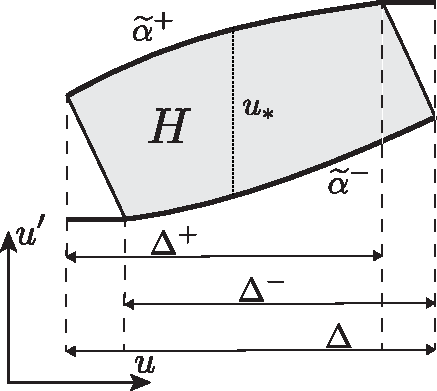
\includegraphics[scale = 1]{pic/thickness definition}
	\caption{An illustration to the definition of an h-strip thickness. Strip $H$ is {\it well-measurable} in a sense of the definition \ref{def:well-measurable}. Curves $\widetilde{\alpha}^{\pm}$ are continuations of the initial h-strip borders to the whole $\Delta$; $u_*$ is a point of maximum of the expression \eqref{eq:h-thickness}.}
\label{fig:thickness-definition}
\end{figure}

\begin{proposition}
	For the \emph{h}-strip $H$ the following statement is valid:
	\begin{equation}
		\Delta^+ \cap \Delta^- \neq \varnothing \Rightarrow u_* \in \Delta^+ \cap \Delta^-,
	\end{equation}
	i.e. an \emph{h}-strip is well-measurable if domains of its border functions have at least one common point.
\end{proposition}
\begin{proof}
	Trivially follows from the monotonicity of the h-strip borders $\alpha^+$ and $\alpha^-$.
\end{proof}

In a similar way we define thickness of v-strips.
Let an v-strip $V$ lies inside an island $D$ and is bounded by v-curves $\beta^+$ and $\beta^-$.
Consider this curves as a functions of $u'$: $u = v_{\pm}(u')$.
Denote domains of these function by $\Delta^{\pm}$.
Continue function $v_{\pm}(u')$ to the whole interval $\Delta = \Delta^+ \cap \Delta^-$ in the same way as for h-strips, see \eqref{eq:continuation}, and introduce new functions $\widetilde{v}_{\pm}(u')$ and curves $\widetilde{\beta}^{\pm}$.

\begin{definition}
	By the {\bf thickness} of an v-strip $V$, denoted $d_\emph{v}(V)$, we mean the distance between curves $\widetilde{\beta}^{\pm}$ in C-norm, i.e.
	\begin{equation}
		d_\emph{v}(V) = d(\widetilde{\beta}^+, \widetilde{\beta}^-) = \max \limits_{u' \in \Delta} |\widetilde{v}_+(u') - \widetilde{v}_-(u')|.
	\label{eq:v-thickness}
	\end{equation}
\end{definition}

The definition of {\it well-measurable} v-strip is introduced in a similar manner.
The remark and the proposition above remain valid for the v-strips as well.
Note that thickness of h-strip is measured in a vertical direction, and thickness of v-strip is measured in a horizontal direction.
If a strip is well-measurable then its thickness is measured in a direction along the straight line that connects points from the opposite side of the strip.
This concept will be useful for us during the proof of a theorem about h,v-strips mapping that we'll formulate somewhat below.

\section{Summary}

% Third chapter
\chapter{Localized Solutions of Gross-Pitaevskii Equation with Periodic Pseudopotential}

\section{Objectives}

In this chapter we apply the coding approach to the Gross-Pitaevskii equation of the form
\begin{equation}
	i \Psi_t + \Psi_{xx} - U(x) \Psi + P(x) |\Psi|^2 \Psi = 0.
\label{eq:gpe}
\end{equation}
Here both potential $U(x)$ and pseudopotential $P(x)$ are periodic functions.
Such equation occurs in physics of Bose-Einstein condensate (BEC) where periodical pseudopotential is achieved by means of the Feshbach resonance controlled by magnetic or optical fields \cite{PollackDriesJunkerChenCorcovilosHulet, ChinGrimmJulienneTsienga, BauerLetterVoRempeDurr}.
Experimentally, the possibility of the periodic modulation of the nonlinearity was demonstrated in \cite{YamazakiTaieSugawaTakahashi}.
One can also find equation \eqref{eq:gpe} in optics where spatial modulation of the Kerr coefficient can be achieved by means of inhomogeneous density of resonant nonlinearity-enhancing dopants implanted into the waveguide \cite{HukriedeRundeKip}.

We are interested in stationary localized solutions of equation \eqref{eq:gpe}, also called as solitons in physical applications.
Strictly speaking, the objects that we are going to study are not solitons in the mathematically rigorous meaning, but rather ``solitary waves'', as they appear in a nonintegrable model.
Nevertheless, the application of the word ``soliton'' to localized pulses in BECs is commonly adopted in physics literature, therefore we also use this word.
Stationary solutions satisfy the ansatz $\Psi(t, x) = u(x) e^{i \omega t}$, where function $u(x)$ is a solution of equation
\begin{equation}
	u_{xx} + Q(x) u + P(x) u^3 = 0, \quad Q(x) = -\omega - U(x).
\end{equation}
Localized solutions satisfy the localization condition
\begin{equation}
	\lim \limits_{x \to \pm \infty} u(x) = 0,
\label{eq:localization}
\end{equation}
which implies that the function $u(x)$ is real, see \cite{AlfimovKonotopSalerno}.
In what follows below we also assume that the potential $U(x)$ is absent, i.e. $U(x) \equiv 0$, so the effects produced by the periodic modulation of the nonlinearity are not obscured by the linear-lattice potential.
Prototypical example of periodic pseudopotential is provided by a function
\begin{equation}
	P(x) = \alpha + \cos 2x, \quad \alpha \in \mathbb{R}.
\label{eq:cosine-pseudopotential}
\end{equation}
Resulting GPE equation takes form
\begin{equation}
	i \Psi_t + \Psi_{xx} + (\alpha + \cos 2x) |\Psi|^2 \Psi = 0,
\label{eq:gpe-cosine}
\end{equation}
where the period of pseudopotential function $P(x)$ is scaled to be $L = \pi$.
Corresponding stationary state equation is
\begin{equation}
	u_{xx} - \omega u + (\alpha + \cos 2x) u^3 = 0.
\label{eq:stationary-cosine}
\end{equation}
Equation \eqref{eq:gpe-cosine} and \eqref{eq:stationary-cosine} are the objects of our analysis during this chapter.
The same model has been previously discussed in literature, see paper \cite{SakaguchiMalomed}.
In \cite{SakaguchiMalomed} only single-peak localized solution, called {\it fundamental soliton} (FS), was studied in details.
For that purpose authors used variational approximation method which requires initial guess of the solution shape.
Such limitation does not allow to find more sophisticated localized solutions.
By using of our coding technique we are going to reveal significantly wider class of stationary localized solutions of Eq.~\eqref{eq:gpe-cosine}.

\section{Coding of Solutions}

Our approach requires the presence of singular solutions families.
That's why according to Proposition~\ref{prop:singular-families} we assume that $\alpha \in (-1; 1)$, so that function $P(x)$ alternates its sing along the value $x$.
We also assume that $\omega > 0$.
This restriction comes from the obvious condition of the soliton localization, given by Eq.\eqref{eq:localization}.

Let's introduce a Poincar\'e map $\mathcal{P}: \mathbb{R}^2 \to \mathbb{R}^2$ associate with equation \eqref{eq:stationary-cosine} in the same way we did it before in \eqref{eq:poincare-map} assuming $L = \pi$.
Poincar\'e map $\mathcal{P}$ and its inverse $\mathcal{P}^{-1}$ is not defined in the whole plane $(u, u')$ of initial conditions.
We can construct their domains using the scanning technique introduced in Chapter~\ref{chapter:II}.
Sets $\mathscr{U}_{\pi}^+$ and $\mathscr{U}_{\pi}^-$ for different parameters $(\omega, \alpha)$ are presented in Figure~\ref{fig:island-set-emergence-cosine}.
Numerical results allows us to conclude that the sets $\mathscr{U}_{\pi}^{\pm}$ are unbounded spirals with infinite number of rotations around the origin, similar to what we saw previously for equation \eqref{eq:stationary-piecewise}.
According to the Proposition~\ref{prop:domain-reflection} these sets are related with a reflection with respect to the $u'$ axis, i.e. $\mathscr{U}_{\pi}^- = I \mathscr{U}_{\pi}^+$.
Their thicknesses depend on the parameter $\alpha$.
If these sets are thin enough their intersection $\mathscr{U}_{\pi} = \mathscr{U}_{\pi}^+ \cap \mathscr{U}_{\pi}^-$ form an island set.
In Figure~\ref{fig:island-set-emergence-cosine} panels (a), (b), and (c) resulting set $\mathscr{U}_{\pi}$ cannot be regarded as island set.
In panel (d) $\mathscr{U}_{\pi}$ is a seven-component island set in the scanning area.

% TODO: Tune colors a bit.
\begin{figure}[h]
\centering
	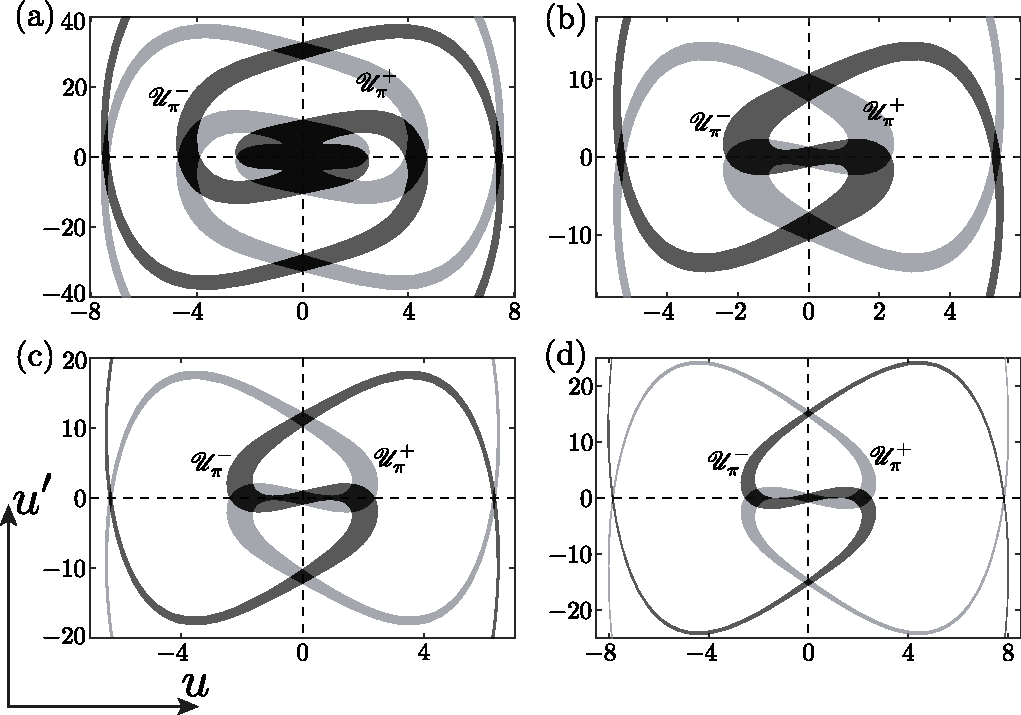
\includegraphics[scale = 1]{pic/island set emergence for cosine equation}
	\caption{
		Sets $\mathscr{U}_{\pi}^+$ (light gray), $\mathscr{U}_{\pi}^-$ (dark gray), and their intersection $\mathscr{U}_{\pi} = \mathscr{U}_{\pi}^+ \cap \mathscr{U}_{\pi}^-$ (black) for equation \eqref{eq:stationary-cosine} with different parameters $(\omega, \alpha)$.
		Panel (a): $(\omega, \alpha) = (1, 0.6)$; panel (b): $(\omega, \alpha) = (1, 0.3)$; panel (c): $(\omega, \alpha) = (1, 0.1)$; panel (d): $(\omega, \alpha) = (1, -0.1)$.
		On panels (a), (b), and (c) intersection $\mathscr{U}_{\pi}$ doesn't form an island set due to the central connected component.
		On panel (d) seven connected components of $\mathscr{U}_{\pi}$ form an island set.
	}
\label{fig:island-set-emergence-cosine}
\end{figure}

Presence of the island set structure is a first required step of our coding technique.
In Chapter~\ref{chapter:II} we established two hypotheses which must be valid, so the conditions of Theorem~\ref{thm:coding} take place.
Let's focus on the case $(\omega, \alpha) = (1.5, 0)$.
We restrict the scanning area in plane $(u, u')$ of initial conditions by seven components of $\mathscr{U}_{\pi}$.
The set $\mathscr{U}_{\pi}$ is depicted in Figure~\ref{fig:island-set-cosine}.
From that picture we conclude that Hypothesis~\ref{hypothesis:island-set} holds since each connected component of $\mathscr{U}_{\pi}$ represent a curvilinear quadrangle with monotonic boundaries, and each boundary satisfies the conditions from Definition~\ref{def:island-set}.
The connected components can be enumerated with symbols $\{D_k\}$, $k = \pm 1, \pm 2, \dots$ for the components along the $u$ axis, and $k = \pm 1\mathrm{i}, \pm 2\mathrm{i}, \dots$ for the components along the $u'$ axis.
The central component is denoted by $D_0$.
Applying this notation for the seven-component island set from Figure~\ref{fig:island-set-cosine} we have $\mathscr{U}_{\pi} = \bigcup_{k \in S_7} D_k$, $S_7 = \{ -2, -1\mathrm{i}, -1, 0, +1, +1\mathrm{i}, +2 \}$.

% TODO: Add squares and dashed lines for the island symbols.
% TODO: Consider to make this figure a little bit larger. Enlarge symbols as well.
\begin{figure}[h]
\centering
	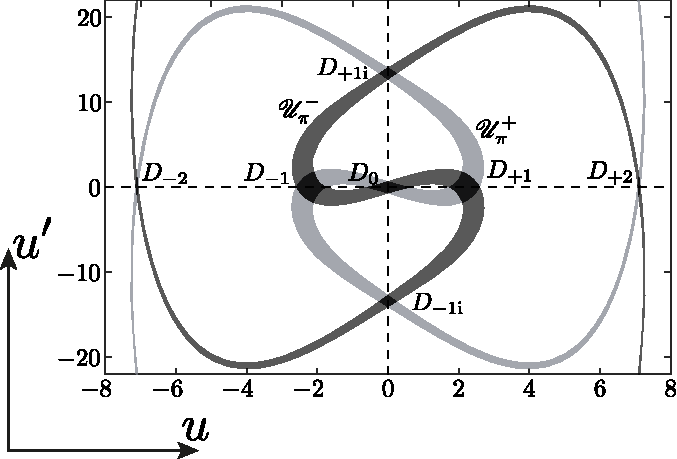
\includegraphics[scale = 1]{pic/island set to check hypotheses for cosine equation}
	\caption{
		Seven-component island set $\mathscr{U}_{\pi} = \bigcup_{k \in S_7}$ (black) formed by the intersection of $\mathscr{U}_{\pi}^{\pm}$ for equation \eqref{eq:stationary-cosine} with parameters $(\omega, \alpha) = (1.5, 0)$.
	}
\label{fig:island-set-cosine}
\end{figure}

To check Hypothesis~\ref{hypothesis:strips-mapping} we use the numerical procedure described in Chapter~\ref{chapter:II} which relies on Strips Mapping Theorems from Appendix~\ref{appendix:strips-mapping-theorems}.
Since set $\mathscr{U}_{\pi}$ is symmetric with respect to the $u$ and $u'$ axis we can check Hypothesis~\ref{hypothesis:strips-mapping} only for four islands: $D_0$, $D_{+1}$, $D_{+2}$, and $D_{+1\mathrm{i}}$.
For each island $D_k$ we introduce a grid of values for numerical computations like we do it during the scanning procedure.
Using that grid we compute sets $H_{i, k} = \mathcal{P}(D_i) \cap D_k$ and sets $V_{k, i} = \mathcal{P}^{-1}(D_i) \cap D_k$, where $i \in S_7$.
In each point $\vb{p} \in V_{k, i}$ we construct a matrix of the 2-dimensional linear operator $D \mathcal{P}_{\vb{p}} = (a_{mn})$.
Then we analyse signs of $(a_{mn})$.
For each set $V_{k, i}$ sings of $(a_{mn})$ must have exactly one configuration specified in Theorem~\ref{thm:h-strips-mapping}.
For each island $D_k$ we also compute a numerical estimation of the lower boundary of $|a_{11}|$ values, denote it by $\mu_*$.
Corresponding histograms of $|a_{11}|$ values in logarithmic scale are presented in Figure~\ref{fig:hypotheses-validation-cosine} along with their lower boundary $\mu_*$ for each island.
Value $\mu_*$ is the numerical estimation of the value $\mu$ from Theorem~\ref{thm:h-strips-mapping}.
If the signs of values $(a_{mn})$ computed for $V_{k, i}$ sets satisfy the conditions of Theorem~\ref{thm:h-strips-mapping} and the overall estimation $\mu_* > 1$ takes place, we conclude that Hypothesis~\ref{hypothesis:strips-mapping} holds true for h-strips.

Similarly, for each set $H_{i, k}$ we construct a matrix of the linear operator $D \mathcal{P}^{-1}_{\vb{p}} = (b_{mn})$ in each point $\vb{p} \in H_{i, k}$.
We perform an estimation of the lower boundary of the values $|b_{22}|$, denote the estimated value by $\nu_*$.
If $\nu_* > 1$ and the signs of values $(b_{mn})$ computed for $H_{i, k}$ sets satisfy the conditions of Theorem~\ref{thm:v-strips-mapping}, we conclude that Hypothesis~\ref{hypothesis:strips-mapping} holds true for v-strips as well.

Complete results of our numerical analysis are presented in Figure~\ref{fig:hypotheses-validation-cosine}.
Let's provide several examples on how this picture should be treated.
Consider an island $D_{+1}$.
Operator $D \mathcal{P}_{\vb{p}} = (a_{mn})$ is computed in each point of the set $V_{+1, 0}$ and has signs configuration $\begin{psm} - & + \\ - & + \end{psm}$ on the whole $V_{+1, 0}$, i.e. $a_{11} < 0$, $a_{12} > 0$, $a_{21} < 0$, $a_{22} > 0$.
Boundaries $\alpha_{+1}^{\pm}$ of the island $D_{+1}$ are the parts of boundaries of $\mathscr{U}_{\pi}^-$ and have the form of decreasing curves, see Figure~\ref{fig:hypotheses-validation-cosine}~(b).
Boundaries $\alpha_0^{\pm}$ of the island $D_0$ are increasing curves.
It means that condition (2d) of Theorem~\ref{thm:h-strips-mapping} takes place for a pair of islands $D_{+1}$ and $D_0$.
For the sets $V_{k, i}$ all the values $|a_{11}| \ge \mu_* > 1$.
Thus, according to Theorem~\ref{thm:h-strips-mapping} we can conclude that for any h-strip $H \in D_{+1}$ its $\mathcal{P}$-image $\widetilde{H}_0 = \mathcal{P}(H) \cap D_0$ is also as h-strip and $d_{\mathrm{h}}(\widetilde{H}_0) \le (1 / \mu_*) d_\mathrm{h}(H)$.

For another example let's consider a pair of islands $D_{+1 \mathrm{i}}$ and $D_{+2}$.
Operator $D \mathcal{P}^{-1}_{\vb{p}} = (b_{mn})$ has sings configuration of the form $\begin{psm} - & - \\ + & + \end{psm}$ for all $\vb{p} \in H_{+1 \mathrm{i}, +2}$.
Boundaries $\beta_{+1 \mathrm{i}}^{\pm}$ of the island $D_{+1 \mathrm{i}}$ are decreasing curves, and boundaries $\beta_{+2}^{\pm}$ of the island $D_{+2}$ are increasing.
Estimations $\nu_* > 1$ takes place for all the sets $H_{i, k}$.
Thus, condition (1d) of Theorem~\ref{thm:v-strips-mapping} is satisfied which implies that and for any v-strip $V \in D_{+2}$ its $\mathcal{P}$-pre-image $\widetilde{V}_{+1 \mathrm{i}} = \mathcal{P}^{-1}(V) \cap D_{+1\mathrm{i}}$ is also a v-strip and $d_{\mathrm{v}}(\widetilde{V}_{+1 \mathrm{i}}) \le (1 / \nu_*) d_\mathrm{v}(V)$.
Other sets $H_{i, k}$, $V_{k, i}$ are considered in a similar way.
According to the numerical computations Theorems~\ref{thm:h-strips-mapping} and \ref{thm:v-strips-mapping} are valid for all islands $D_k$, $k \in S_7$.

% TODO: Take care of the position for this figure.
\begin{figure}[h!]
\centering
	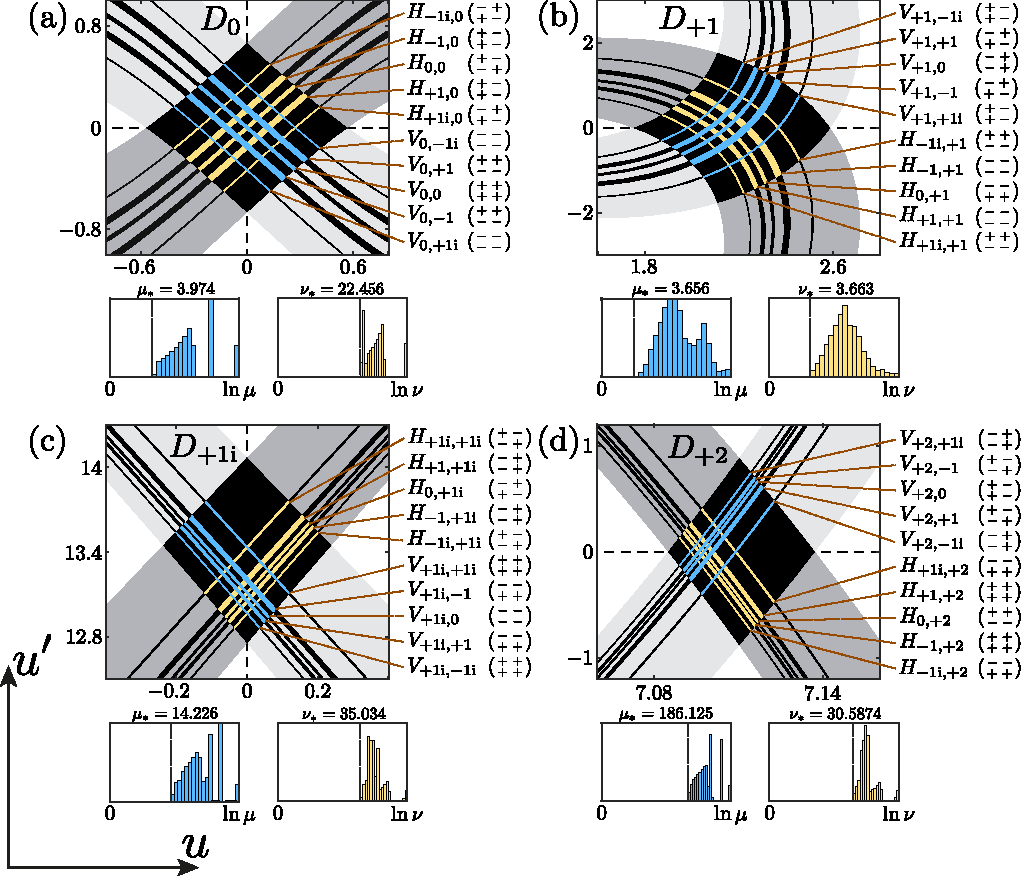
\includegraphics[scale = 1]{pic/hypotheses for cosine equation}
	\caption{
		Illustration to Hypothesis~\ref{hypothesis:strips-mapping} validation for equation \eqref{eq:stationary-cosine} with parameters $(\omega, \alpha) = (1.5, 0)$.
		Islands $D_k$ are black curvilinear quadrangles with monotonic boundaries.
		Boundaries of the set $\mathscr{U}_{\pi}^+$ (light gray) contains $\beta_k^{\pm}$ boundaries for each island $D_k$; boundaries of $\mathscr{U}_{\pi}^-$ (dark gray) contains $\alpha_k^{\pm}$ boundaries correspondingly.
		Estimations of $\mu_*$ and $\nu_*$ values are shown with histograms below each island.
		Configuration of value signs in operators $D \mathcal{P}_{\vb{p}} = (a_{mn})$, $\vb{p} \in V_{k, i}$ (blue), and $D \mathcal{P}^{-1}_{\vb{p}} = (b_{mn})$, $\vb{p} \in H_{i, k} $ (yellow) are shown from the right side of each island $D_k$.
		All of them satisfy the conditions of Theorem~\ref{thm:h-strips-mapping} (On h-strip mapping) and Theorem~\ref{thm:v-strips-mapping} (On v-strips mapping) from Appendix~\ref{appendix:strips-mapping-theorems}.
		Sets $H_{+2, k}$ and $V_{k, +2}$ are not depicted since they are too thin and barely visible at this scale, but all the computations have been also provided for them and the overall result satisfies the above mentioned theorems as well.
	}
\label{fig:hypotheses-validation-cosine}
\end{figure}

The procedure described above provides a numerical evidence for Hypotheses~\ref{hypothesis:island-set} and \ref{hypothesis:strips-mapping}.
That allows us to apply Coding Theorem and conclude that for Eq.~\eqref{eq:stationary-cosine} there exists a homeomorphism $\mathcal{C}: \mathcal{O}_7 \to \mathcal{S}_7$ between a subset of orbits of bounded solutions, denoted by $\mathcal{O}_7$, and a set $\mathcal{S}_7$ of bi-infinite sequences of symbols from alphabet $S_7 = \{ -2, -1\mathrm{i}, -1, 0, +1, +1\mathrm{i}, +2 \}$.
Orbits of such solutions may visit only islands $D_k$, where $k \in S_7$.
Moreover there is no any other bounded solution which orbit visits only these seven islands.
The numerical results from above can be extended to a larger island set, although it requires significant computing capacities.

Existence of the homeomorphism allows to make a conclusion on the structure of bounded solutions of Eq.~\ref{eq:stationary-cosine} 
For example Eq.~\ref{eq:stationary-cosine} admits periodic solution of period $n \pi$ for any number $n \in \mathbb{N}$.
Several periodic solutions are presented in Figure~\ref{fig:solutions-cosine}, $\pi$-periodic solution in panel (a), and $2 \pi$-periodic solutions in panels (b) and (c).
There also exists a plethora of soliton solutions.
The orbit corresponding to the soliton solution starts and ends in the central connected components; therefore, it has the code of the form $\{ \dots, 0, 0, k_1, k_2, \dots, k_N, 0, 0, \dots \}$, where symbols $k_1$ and $k_N$ are different from ``$0$''.
Some of the soliton solutions of \eqref{eq:stationary-cosine} for $(\omega, \alpha) = (1.5, 0)$ are shown in Figure~\ref{fig:solutions-cosine}, panels (d) --- (i).
The soliton solution in panel (d) is the fundamental soliton (FS) that has been already studied in \cite{SakaguchiMalomed}.
It has code $\{ \dots 0, +1, 0, \dots \}$, or $\{ \dots 0, -1, 0, \dots \}$ which is its symmetric counterpart.

Other types of localized solutions have been also found.
For example, solution, shown in panel (e), represents a so-called {\it dipole soliton} (DS) \cite{LebedevAlfimovMalomed}, which is essentially confined to a single period of pseudopotential $P(x)$.
This solution corresponds to code $\{ \dots, 0, -1\mathrm{i}, 0, \dots \}$, and its symmetric counterpart is $\{ \dots, 0, +1\mathrm{i}, 0, \dots \}$.
DS is similar to {\it sub-fundamental solitons} (SFSs) reported in \cite{MayteevarunyooMalomed, WangYanLiu, MayteevarunyooMalomedBaizakovSalerno, CuevasMalomedKevrekidisFrantzeskakis} in models with the linear lattice potential $U(x)$, as both soliton species feature the antisymmetric profile squeezed into a single cell of the underlying lattice potential (ordinary potential $U(x)$, in the case of SFS, and the pseudopotential $P(x)$, as concerns the DS).
The area of the localization of the soliton corresponding to code $\{ \dots, 0, k_1, \dots, k_N, 0, \dots \}$, where the symbols $k_1$ and $k_N$ are different from ``$0$'', is $N \pi$, i.e. it extends over $N$ periods of the underlying pseudopotential $P(x)$.
In particular, the solitons with codes $\{ \dots, 0, k, 0, \dots \}$, $k \ne 0$ (named {\it elementary solitons}), are localized, essentially, in one period of the pseudopotential. 

\begin{figure}[h]
\centering
	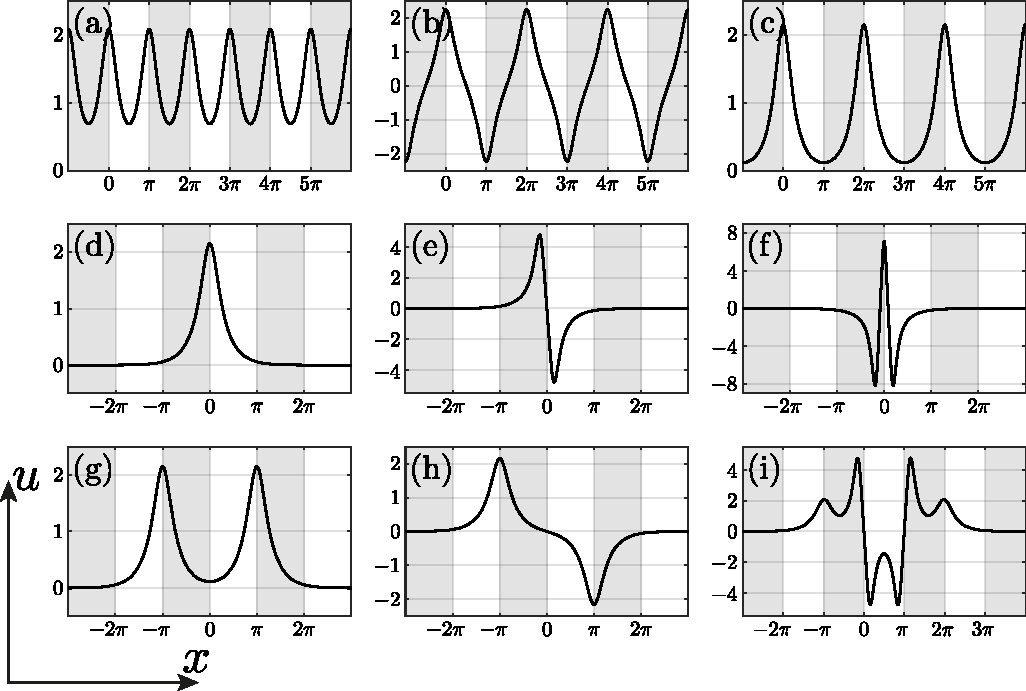
\includegraphics[scale = 1]{pic/solutions for cosine equation}
	\caption{
		Different solutions for equation \eqref{eq:stationary-cosine} with parameters $(\omega, \alpha) = (1.5, 0)$.
		Each solution has a corresponding symbolic code, this code identify the solution uniquely.
		Gray strips divide the $x$ axis according to the period $\pi$.
		First three panels represent periodic solutions, their codes have periodic structure: (a) $\pi$-periodic solution $\{ \dots, +1, +1, +1, \dots \}$; (b) $2 \pi$-periodic solution $\{ \dots, +1, -1, +1, -1, \dots \}$; (c) $2 \pi$-periodic solution $\{ \dots, +1, 0 +1, 0, \dots \}$.
		Other six panels represent localized solutions, their codes have ``$0$'' symbol to the left and right of the central block: (d) fundamental soliton with code $\{ \dots, 0, +1, 0, \dots \}$; (e) dipole soliton with code $\{ \dots, 0, -1\mathrm{i}, 0, \dots \}$ (f) elementary soliton with code $\{ \dots, 0, +2, 0, \dots \}$ (g) $\{ \dots, 0, +1, 0, +1, 0, \dots \}$ (h) $\{ \dots, 0, +1, 0, -1, 0, \dots \}$ (i) $\{ \dots, 0, +1, -1\mathrm{i}, +1\mathrm{i}, +1, \dots \}$.
	}
\label{fig:solutions-cosine}
\end{figure}

\section{Analysis of Stability}

Stability is a critically important issue for stationary localized solutions.
By stability of localized stationary solution we mean its resistance to small perturbations.
From the perspective of real physical experiments only stable solutions can be obtained in a real experimental setup.
Here we address the stability of stationary localized solutions produced by Eq.~\eqref{eq:gpe-cosine}.
Let $u(x)$ be a solution if Eq.~\eqref{eq:stationary-cosine}.
Following the well-established approach, see e.g. \cite{JiankeYang}, let's consider small perturbations around a solution $u(x)$ of the form
\begin{equation}
	\Psi(t, x) = \left( u(x) + \widetilde{U}(t, x) \right) e^{i \omega t}; \quad |\widetilde{U}(t, x)| \ll 1,
\label{eq:perturbation}
\end{equation}
where $\widetilde{U}(t, x)$ is a complex-valued function.
Then the perturbation $\widetilde{U}(t, x)$ satisfies the linear equation
\begin{equation}
	i \widetilde{U}_t + \widetilde{U}_{xx} - \omega \widetilde{U} + (\alpha + \cos 2x) u^2 (2 \widetilde{U} + \widetilde{U}^\dagger) = 0.
\label{eq:perturbation-equation}
\end{equation}
Here dagger ``$\dagger$'' means complex conjugate.
Seeking solutions to \eqref{eq:perturbation-equation} as
\begin{equation}
	\widetilde{U}(t, x) = (a(x) + w(x)) e^{\lambda t} + (v^{\dagger}(x) - w^{\dagger}(x)) e^{\lambda^{\dagger} t}; \quad \lambda \in \mathbb{C},
\end{equation}
we arrive at the eigenvalue problem
\begin{equation}
	i
	\begin{pmatrix}
		0 & \partial_{xx} + G_1(x) \\
		\partial_{xx} + G_2(x) & 0
	\end{pmatrix}
	\begin{pmatrix}
		v \\
		w
	\end{pmatrix}
	= \lambda 
	\begin{pmatrix}
		v \\
		w
	\end{pmatrix},
\label{eq:eigenvalue-problem}
\end{equation}
where
\begin{eqnarray*}
	&& G_1(x) = -\omega + (\alpha + \cos 2x) u^2; \\
	&& G_2(x) = -\omega + 3 (\alpha + \cos 2x) u^2.
\end{eqnarray*}

Equation \eqref{eq:eigenvalue-problem} is the linear-stability eigenvalue problem for the soliton.
Its $\lambda$-spectrum is called the linear-stability spectrum for this soliton.
The soliton is linearly stable if the spectrum produced by Eq.~\eqref{eq:eigenvalue-problem} contains at least one eigenvalue $\lambda$ with a non-zero real part, $\mathfrak{R}(\lambda) > 0$.
Otherwise, the soliton is linearly stable.
Equation \eqref{eq:eigenvalue-problem} generates spectrum consisting of continuous and discrete parts.
One can show, see e.g. \cite{JiankeYang}, that the continuous spectrum is represented by two rays, $[i\omega; +i \infty)$ and $(-i \infty; -i \omega]$, if $\omega > 0$, and by the whole imaginary axis, if $\omega < 0$.
The discrete spectrum includes zero eigenvalue $\lambda = 0$.
It is easy to see that other eigenvalues of discrete spectrum of Eq.~\eqref{eq:eigenvalue-problem} have the following symmetry properties: if $\lambda$ is an eigenvalue, then so are $\lambda^{\dagger}$, $-\lambda$, and $-\lambda^{\dagger}$.
This means that these eigenvalues always appear in pairs or quadruples.

\subsection{Fourier Collocation Method}

To find discrete eigenvalues numerically we use so-called Fourier Collocation Method (FCM) described in \cite{JiankeYang}.
This method is very efficient to find {\it exponential instabilities} that appear due to real eigenvalues.
We also say that solution {\it oscillatory unstable} if the spectrum has quartets of complex with non-zero real parts.

To apply FCM, we first truncate the infinite $x$-axis into a finite interval into  a finite interval $[-L/2; L/2]$, where $L$ is the length of the interval.
Length of the interval is considered to be large enough to cover soliton solution localization well.
On this interval we expand the eigenfunctions $[v(x); w(x)]^T$ and functions $G_1$, $G_2$ into Fourier series:
\begin{eqnarray*}
	&& 	v(x) = \sum \limits_n a_n e^{i n k_0 x}; \quad w(x) = \sum \limits_n b_n e^{i n k_0 x}, \label{eq:eigenfunctions-expansion} \\
	&& G_1 = \sum \limits_n c_n^{(1)} e^{i n k_0 x}; \quad G_2 = \sum \limits_n c_n^{(2)} e^{i n k_0 x} \label{eq:g-functions-expansion},
\end{eqnarray*}
where $k_0 = 2 \pi / L$.
After substitution of \eqref{eq:eigenfunctions-expansion} and \eqref{eq:g-functions-expansion} into \eqref{eq:eigenvalue-problem}, we have the following eigenvalue system fro the coefficients $a_j$, $b_j$:
\begin{eqnarray}
	&& -(k_0 j)^2 b_j + \sum \limits_n 	c_n^{(1)} b_{j - n} = -i \lambda a_j; \\
	&& -(k_0 j)^2 a_j + \sum \limits_n 	c_n^{(2)} a_{j - n} = -i \lambda b_j,
\end{eqnarray}
where $-\infty < j < +\infty$.
Truncating the number of Fourier modes to $-N \le j \le N$, this infinite-dimensional eigenvalue problem can be reduced to the finite-dimensional one:
\begin{equation}
	i
	\begin{pmatrix}
		0 & D + C_1 \\ D + C_2 & 0
	\end{pmatrix}
	\begin{pmatrix}
		A \\ B
	\end{pmatrix}
	= \lambda
	\begin{pmatrix}
		A \\ B
	\end{pmatrix},
\label{eq:eigenvalue-problem-matrix}
\end{equation}
where
\begin{eqnarray*}
	&& D = (ik_0)^2 \mathrm{diag}(-N, -N+1, \dots, N-1, N)^2; \\
	&& A = (a_{-N}, a_{-N+1}, \dots, a_N)^T; \quad B = (b_{-N}, b_{-N+1}, \dots, b_N)^T,
\end{eqnarray*}
and matrices $C_1$, $C_2$ are of the form of Toeplitz matrices
\begin{equation}
	C_{1,2} =
	\begin{pmatrix}
		c_0^{(1,2)} & c_{-1}^{(1,2)} & \cdots & c_{-N}^{(1,2)} & 0 & \cdots & 0 \\
		c_1^{(1,2)} & c_0^{(1,2)} & c_{-1}^{(1,2)} & \ \ddots & \ddots & \ddots & \vdots \\
		\vdots & c_1^{(1,2)} & c_0^{(1,2)} & c_{-1}^{(1,2)} & \ddots & \ddots & 0 \\
		c_N^{(1,2)} & \ddots & \ddots & \ddots & \ddots & \ddots & c_{-N}^{(1,2)} \\
		0 & c_N^{(1,2)} & \ddots & \ddots & \ddots & \ddots & \vdots \\
		\vdots & \ddots & \ddots & \ddots & \ddots & \ddots & \vdots \\
		0 & \cdots & 0 & c_N^{(1,2)} & \cdots & c_1^{(1,2)} & c_0^{(1,2)}
	\end{pmatrix}.
\end{equation}
The matrix eigenvalue problem \eqref{eq:eigenvalue-problem-matrix} can be solved by any matrix eigenvalue problem solver.
Solution of the eigenvalue problem gives $2N + 1$ eigenvalues.
In our computations we used $N = 256$ and $N = 512$ and got nearly identical spectrums.
From the practical point of view for the linear-stability analysis the number of Fourier modes can be relatively small, since eigenvalues for the higher modes have zero real part.

\subsection{Evolutionary Simulation}

To control linear-stability analysis and get additional confidence in stability of localized solutions we also performed a numerical simulation of their evolution.
For that purpose Trofimov-Peskov finite-difference scheme \cite{TrofimovPeskov} for numerical solution of the Gross-Pitaevskii \eqref{eq:gpe} equation was used. 
The scheme preserves several invariants of the problem: the norm of the solution
\begin{equation}
	N = \int \limits_{-\infty}^{+\infty} |u(x)|^2 dx,
\label{eq:norm}
\end{equation}
and its energy
\begin{equation}
	E = \int \limits_{-\infty}^{+\infty} \left( |u'(x)|^2 + U(x) |u(x)| - \dfrac{1}{2} P(x) |u(x)|^4 \right) dx.
\label{eq:energy}
\end{equation}
The scheme is implicit, its realization implying iterations for the calculation of values in each temporal layer, but it allows running computation with larger temporal step.
In order to reveal instability (if it is), the soliton profile was perturbed at the initial moment with a small perturbation.
A finite spatial domain $[-5 \pi; 5 \pi]$ was used, with reflection of radiation from boundaries eliminated by means of absorbing boundary conditions.
During our analysis we got consistent results between the linear stability and evolutionary simulation.

\subsection{Results of Linear Stability Analysis}

With the help of FCM, a great number of localized stationary solutions of equation \eqref{eq:gpe-cosine}, represented by different codes, were analyzed.
Due to the infinite number of essentially different solitons, it's not possible to preform a comprehensive stability analysis of all localized solutions.
However, we observed that a majority of the solitons are linearly unstable, thus being physically irrelevant solutions.
{\it Stable solitons} can be categorized as follows:
\begin{itemize}
	\item[(a)] among the elementary solitons, it was found that FS and DS are {\it linearly stable}, under some restrictions on parameters $\omega$ and $\alpha$, while other elementary solitons were found to be unstable;
	\item[(b)] there are stable localized solutions of the form of FS complexes --- for instance, with codes $\{ \dots, 0, +1, -1, +1, 0, \dots \}$ and $\{ \dots, +1, 0, -1, 0, \dots \}$.
\end{itemize}

\begin{figure}[h!]
\centering
	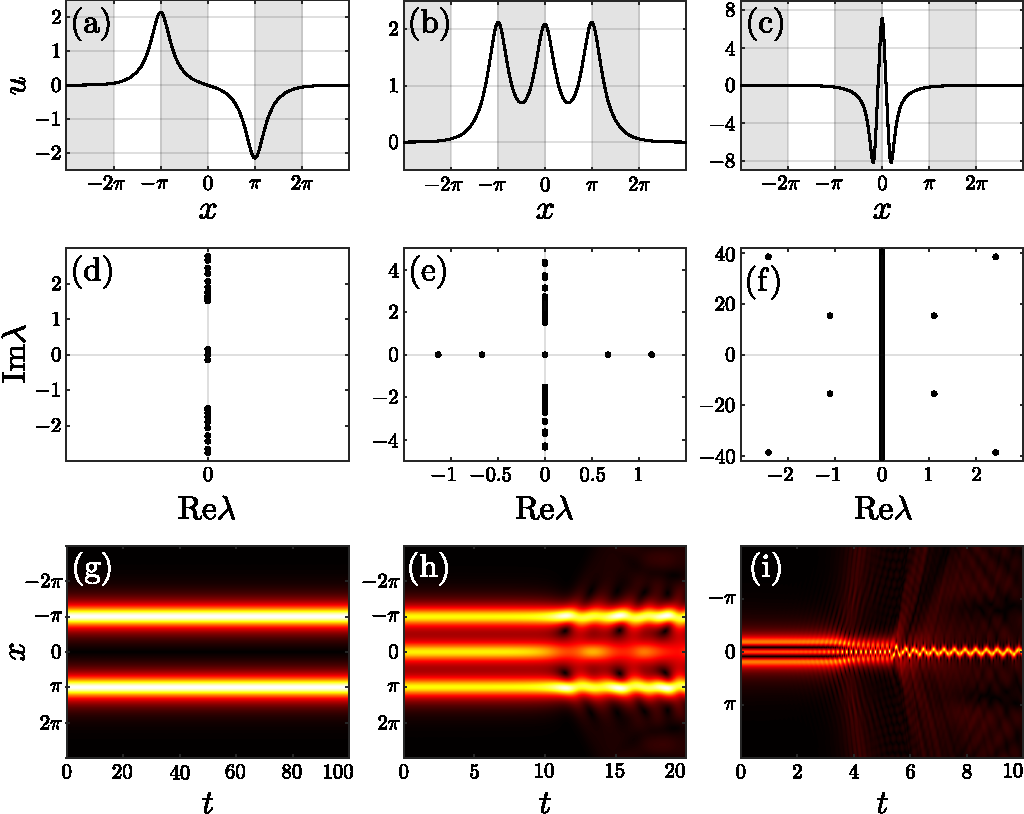
\includegraphics[scale = 1]{pic/stability demonstration for cosine equation}
	\caption{
		Examples of stability analysis for localized solutions of equation \eqref{eq:gpe-cosine} with parameters $(\omega, \alpha) = (1.5, 0)$.
		First three panels represent profiles of solutions of different codes: (a) $\{ \dots, 0, +1, 0, -1, 0, \dots \}$; (b) $\{ \dots, 0, +1, +1, +1, 0, \dots \}$; (c) $\{ \dots, 0, +2, 0, \dots \}$.
		Panels (d), (e), and (f) are the corresponding $\lambda$-spectrums for the solutions above.
		According to them, solution in panel (a) is linearly stable.
		Solution in panel (b) is exponentially unstable, while solution in panel (c) is oscillatory unstable.
		Linear-stability analysis match the results of evolutionary simulation presented in panel (g), (h), and (i).
	}
\label{fig:stability-cosine}
\end{figure}

Several localized solution, their linear-stability spectrums, and corresponding results of evolutionary simulation are in Figure~\ref{fig:stability-cosine}.
Panel (a) corresponds to a stable localized solution of code $\{ \dots, 0, +1, 0, -1, 0, \dots \}$.
Such solution can be considered as a combination of two FSs of codes $\{ \dots, 0, +1, 0, \dots \}$ and $\{ \dots, 0, -1, 0, \dots \}$.
Another similar combination of code $\{ \dots, 0, +1, +1, +1, 0, \dots \}$ in panel (b) is unstable.
Elementary soliton of code $\{ \dots, 0, +2, 0, \dots \}$ from panel (c) is unstable as well as any other elementary solitons except of FS and DS.
Other examples can be found in our work \cite{LebedevAlfimovMalomed}.

Combination of coding technique and linear-stability analysis together give a powerful tool of visualization of stationary localized solutions stability for equation of type \eqref{eq:gpe} with periodic potential and pseudopotential.
If it's possible to find such parameters that the Theorem~\ref{thm:coding} is applicable, then for these parameters we can apply coding and describe at least a huge subset of bounded solutions.
After that one can vary one of the parameters using a numerical grid and perform a numerical continuation for the described solutions to the non-coding area of parameters.
During the numerical continuation of solutions we can compute linear-stability spectrums in each point of the parameters grid.
Then we can parametrized the obtained solutions, for example using their norm \eqref{eq:norm}, plot the branches of different solution families and color the stability regions.

Illustration of the described idea for Eq.~\eqref{eq:gpe-cosine} is presented in Figure~\ref{fig:branches-with-stability}.
In that figure several branches of solutions are depicted in $(N, \omega)$ axes, while parameter $\alpha = 0$.
Regions of linear stability are marked with bold black lines.
One can see that FS solution of code $\{ \dots, 0, \pm 1, 0, \dots \}$, branch (I), and solution of code $\{ \dots, 0, \pm 1, 0 \mp 1, 0, \dots \}$, branch (II), are mostly stable and loose their stability near the point $\omega = 0$.
Dipole soliton, branch (IV), exists for $\omega > \omega^*$ and has an $\omega$-region of stability.
At $\omega^* \approx 0.265$, the DS family, coded by $\{ \dots, 0, \pm 1\mathrm{i}, 0, \dots \}$, undergoes a saddle-node bifurcation and annihilate with the family coded by $\{ \dots, 0, \mp 1, \pm 1\mathrm{i}, \pm 1, 0, \dots \}$.

\begin{figure}[h]
\centering
	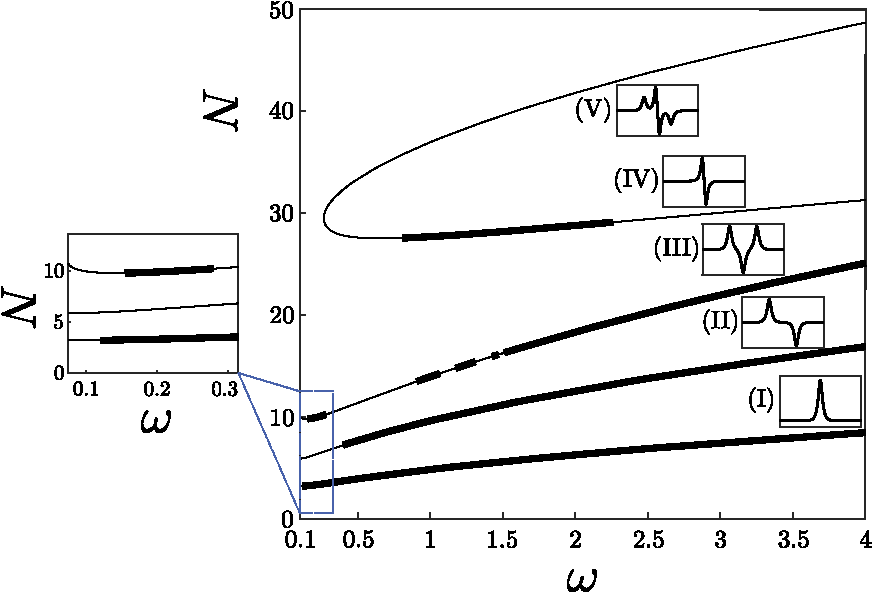
\includegraphics[scale = 1]{pic/branches for cosine equation}
	\caption{
		Branches of solutions for Eq.~\eqref{eq:gpe-cosine} and their linear stability.
		Branch (I) represent fundamental soliton family of code $\{ \dots, 0, \pm 1, 0, \dots \}$.
		Branches (II) and (III) are FS complexes of codes $\{ \dots, \pm 1, 0, \mp 1, 0, \dots \}$ and $\{ \dots, \pm 1, \mp 1, \pm 1, 0, \dots \}$ correspondingly.
		Dipole soliton family of code $\{ \dots, 0, \pm 1\mathrm{i}, 0, \dots \}$ is presented by the branch (IV).
		It coalesces at $\omega = \omega^*$ with family $\{ \dots, 0, \mp 1, \pm 1\mathrm{i}, \pm 1, 0, \dots \}$ of branch (V).
		Linear stability regions are colored with bold black lines.
	}
\label{fig:branches-with-stability}
\end{figure}

\subsubsection{Stable Dipole Soliton}

As an outcome of our analysis for physical applications, the most significant finding is the existence of stable DS family, which was not previously considered in the setting of GPE with periodic pseudopotential.
Existence of such family is also predicted by variational approximation method, see \cite{LebedevAlfimovMalomed}.
The DS family may be parametrized by $\omega$.
The norm of the DS grows with the growth of $\omega$.
Although the DS is very similar, in its shape, to the sub-fundamental solitons in systems with periodic potential, the DS in the present model is not sub-fundamental, as its norm os {\it higher} than that of the FS existing for the same $\omega$, see Figure~\ref{fig:branches-with-stability}.
Evolutionary simulation showed that if for some $\omega$ the DS is unstable, then it transforms into the FS after some time.
An example of that is provided in Figure~\ref{fig:stability-dipole-soliton}.

\begin{figure}[h]
\centering
	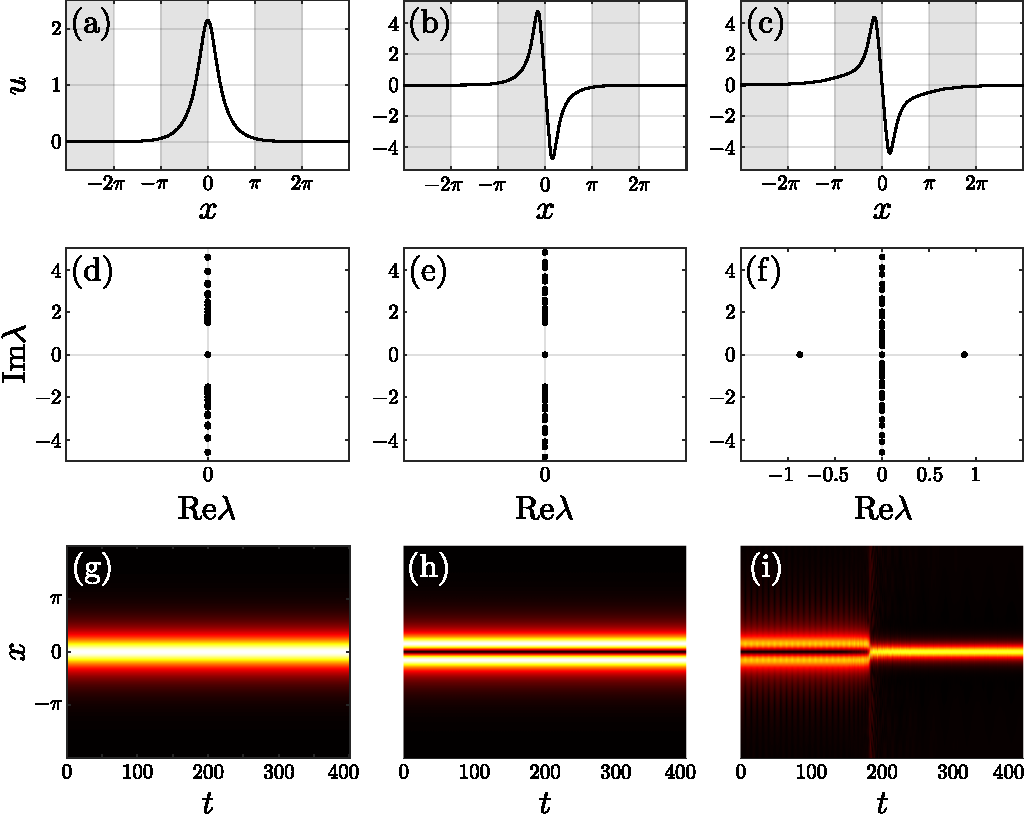
\includegraphics[scale = 1]{pic/dipole soliton stability}
	\caption{
		Stability of dipole soliton.
		Panel (a) represent a stable fundamental soliton (FS) for parameters $(\omega, \alpha) = (1.5, 0)$.
		Panel (b) corresponds to stable dipole soliton (DS) for $(\omega, \alpha) = (1.5, 0)$.
		Unstable DS is presented in panel (c) for parameters $(\omega, \alpha) = (0.4, 0)$.
		It's exponentially unstable and  during our simulation at $t \approx 200$ transforms into a stable fundamental soliton.
	}
\label{fig:stability-dipole-soliton}
\end{figure}

\section{Summary}

In this chapter we studied stationary solutions of Gross--Pitaevskii equation \eqref{eq:gpe} with presence of periodic pseudopotential $P(x)$ of the cosine form \eqref{eq:cosine-pseudopotential}, while potential $U(x)$ is absent.
We focused on localized solutions as they are of particular interest for physical experiments.
Periodicity of pseudopotential $P(x)$ allowed us to apply coding technique from Chapter~\ref{chapter:II}.
We provided a numerical evidence for Hypotheses~\ref{hypothesis:island-set} and \ref{hypothesis:strips-mapping}, which allow to apply Theorem~\ref{thm:coding}, and concluded that there exist a homeomorphism between a subset of bounded solutions and bi-infinite symbolic sequences from some alphabet.
Existence of the homeomorphism reveal the complex nature of stationary solutions. 
Like we saw it in Chapter~\ref{chapter:II} presence of periodic pseudopotential that alters its sign along the period generates a great variety of different stationary solutions.
We apply linear-stability analysis to identify physically relevant localized solutions among them.
Outcome of our analysis is the existence of stable dipole soliton (DS) family previously not considered in this setting.
Results of our finding were published in \cite{LebedevAlfimovMalomed}.


% Fourth chapter
% TODO: $\Gamma_n^{\Omega}$ is ugly notation. May it's worth to fix it somehow?
% TODO: "parabolic-pseudopotential" to "periodic-pseudopotential".
% TODO: Check all references and labels again.

\chapter{Localized Solutions of Nonlinear Harmonic Oscillator with Periodic Pseudopotential}

\section{Objectives}

In this chapter we study localized solutions of Gross--Pitaevskii equation with a harmonic-oscillator (parabolic) trapping potential and a periodic pseudopotential in front of cubic term.
The effective one-dimensional GPE for mean-fields wave function $\Psi(t, x)$ is
\begin{equation}
	i \Psi_t + \Psi_{xx} - \dfrac{1}{2} a^2 x^2 \Psi + P(x) |\Psi|^2 \Psi = 0,
\label{eq:gpe-parabolic-non-scaled}
\end{equation}
where $a^2$ is the strength of the harmonic-oscillator potential, and pseudopotential $P(x)$ is a function of period $L = 2 \pi / \Omega$:
\begin{equation}
	P(x + 2 \pi / \Omega) = P(x).
\end{equation}
Such model can be achieved by means of combination of a magnetic trap and an optical lattice which induces the periodic pseudopotential via the Feshbach resonance \cite{SakaguchiMalomed2010}.
Intervals with positive (negative) values of $P(x)$ correspond to spatial domains with attractive (repulsive) interactions between particles.

The model includes {\it two scales}: the characteristic harmonic-oscillator length $l_{\mathrm{HO}} \sim 1 / \sqrt{a}$, and period $L = 2 \pi / \Omega$ of the pseudopotential.
In particular, the limit case of the wide harmonic-oscillator trap $\Omega \gg 2 \pi \sqrt{a}$, is a physically relevant one.
Let's introduce additional rescaling
\begin{equation}
	t \to \dfrac{a}{\sqrt{2}} t, \quad x \to \dfrac{\sqrt{a}}{\sqrt[4]{2}} x, \quad \Psi \to \dfrac{\sqrt[4]{2}}{\sqrt{a}} \Psi.
\end{equation}
This allows to fix $a \equiv 1$ and convert \eqref{eq:gpe-parabolic-non-scaled} into a normalized form
\begin{equation}
	i \Psi_t + \Psi_{xx} - x^2 \Psi + P(x) |\Psi|^2 \Psi = 0,
\label{eq:gpe-parabolic}
\end{equation}
where $P(x)$ is periodic with spatial frequency $\widetilde{\Omega} = \Omega / \sqrt{a}$.
In what follows below, symbol $\widetilde{\Omega}$ is replaced by $\Omega$.
To estimate physically relevant values of $\Omega$ we use the results of experimental realization of the periodically-modulated Feshbach resonance in \cite{YamazakiTaieSugawaTakahashi}.
There the corresponding scaled spatial frequency being $\Omega \sim 100$.
It can be made smaller, taking larger $a$.

Equation \eqref{eq:gpe-parabolic} is our basic model.
The objective of our analysis is to study its localized stationary solutions of the form
\begin{equation}
	\Psi(t, x) = u(x) e^{-i \omega t},
\end{equation}
where real-valued function $u(x)$ satisfies equation
\begin{equation}
	u_{xx} + (\omega - x^2) u + P(x) u^3 = 0
\label{eq:nho-periodic}
\end{equation}
with localization boundary conditions
\begin{equation}
	\lim \limits_{x \to \pm \infty} u(x) = 0.
\end{equation}
During our numerical analysis we focus on the practically important case when the pseudopotential function $P(x)$ in \eqref{eq:gpe-parabolic} is taken as a sum of constant and harmonic parts of a prototypical cosine form:
\begin{equation}
	P(x) = P_0 + P_1 \cos (\Omega x).
\label{eq:gpe-parabolic-pseudopotential}
\end{equation}

As we say it in Chapter~\ref{chapter:III} stability of solutions is a critically important property.
Linear stability of localized solutions is addressed by considering of small perturbations of a solution $u(x)$ of the form:
\begin{equation}
	\Psi(t, x) = \left( u(x) + (v(x) + w(x)) e^{\lambda t} + (v^{\dagger}(x) - w^{\dagger}(x)) e^{\lambda^{\dagger} t} \right) e^{-i \omega t},
\label{eq:gpe-parabolic-perturabation}
\end{equation}
where $|v(x)| \ll 1$, $|w(x)| \ll 1$.
Substituting \eqref{eq:gpe-parabolic-perturabation} into \eqref{eq:gpe-parabolic} and performing linearization with respect to $v(x)$ and $w(x)$, we arrive at eigenvalue problem
\begin{equation}
	i
	\begin{pmatrix}
		0 & \mathcal{L}_- \\
		\mathcal{L}_+ & 0
	\end{pmatrix}
	\begin{pmatrix}
		v \\ w
	\end{pmatrix} =
	\lambda
	\begin{pmatrix}
		v \\ w	
	\end{pmatrix},
\label{eq:eigenvalue-problem-gpe-parabolic}
\end{equation}
where 
\begin{eqnarray*}
	&& \mathcal{L}_- = \partial_{xx} + \omega -x^2 + P(x) u^2; \\
	&& \mathcal{L}_+ = \partial_{xx} + \omega -x^2 + 3 P(x) u^2.
\end{eqnarray*}
This problem is similar to the previously considered problem \eqref{eq:eigenvalue-problem}.
Fourier Collocation Method from Chapter~\ref{chapter:III} is also applicable for effective numerical evaluation of spectrum \eqref{eq:eigenvalue-problem-gpe-parabolic}.
Eigenvalues with non-zero real part rise to the instability, while pure imaginary spectrum indicates that solutions is linearly stable.
Again, we note that the eigenvalues appears in pairs and quadruples, i.e. if $\lambda$ is an eigenvalue, then $-\lambda$, $\lambda^{\dagger}$, $-\lambda^{\dagger}$ are eigenvalues too.

For the analytical analysis during this chapter it's convenient to rewrite eigenvalue problem \eqref{eq:eigenvalue-problem-gpe-parabolic} in the equivalent form:
\begin{equation}
	\mathcal{L}_+ \mathcal{L}_- w = \Lambda w, \quad \Lambda = -\lambda^2.
\label{eq:eigenvalue-problem-gpe-parabolic-analytical}
\end{equation}
In terms of \eqref{eq:eigenvalue-problem-gpe-parabolic-analytical}, a solution $u(x)$ passes the linear stability test if the spectrum of eigenvalues $\Lambda$ is all-real positive.

\subsection{Solutions with linear counterpart}

An important class of localized solutions of equation \eqref{eq:nho-periodic} is {\it nonlinear solutions with linear counterpart}.
Such terminology has been adopted in \cite{AgostaMalomedPresilla, AgostaPresilla}.
Existence of such solution came from the consideration of the low-amplitude limit.
% TODO: Add reference to the definition of norm from the overall introduction, not from Chapter III.
For a small value of norm $N$, see \eqref{eq:norm}, the nonlinear term in \eqref{eq:nho-periodic} may be neglected, which leads to the ordinary harmonic-oscillator equation
\begin{equation}
	u_{xx} + (\omega - x^2) u = 0.
\label{eq:ho}
\end{equation}
Equation \eqref{eq:ho} produces the commonly known set of eigenvalues and eigenfunctions:
\begin{equation}
	\tilde{\omega}_n = 2n + 1; \quad \tilde{u}_n(x) = \dfrac{1}{\sqrt{2^n n! \sqrt{\pi}}} H_n(x) e^{-\frac{1}{2} x^2}; \quad n = 0, 1, \dots,
\label{eq:ho-solutions}
\end{equation}
where $H_n(x)$ functions are Hermite polynomials.
In particular,
\begin{equation*}
	H_0(x) = 1, \quad H_1(x) = 2x, \quad H_2(x) = 4x^2 - 2.	
\end{equation*}

When the nonlinearity is switched on, each linear eigenstate $(\tilde{\omega}_n, \tilde{u}_n(x))$ bifurcates into a one-parameter set $\Gamma_n = (\omega_n, u_n(x))$ of small-amplitude localized solutions of \eqref{eq:nho-periodic}.
These solutions are produced by equation \eqref{eq:nho-periodic} and become essentially nonlinear with the increase of $N$ and distance between $\omega_n$ and $\tilde{\omega}_n$.
Localized solutions from family $\Gamma_n$ feature the same parity as the corresponding linear eigenfunction $\tilde{u}_n(x)$, solution with even $n$ are even functions of $x$, and those with the odd $n$ are odd.
Localized solution with $n = 0$ originates form the ground state of the harmonic-oscillator.

During our analysis it's interesting to compare the results with the well-studied case of Gross--Pitaevskii equation \eqref{eq:gpe-parabolic} with constant $P(x)$ (negative or positive).
In this case $P_1 \equiv 0$ in \eqref{eq:gpe-parabolic-pseudopotential}, and after additional rescaling $\Psi \to \Psi / \sqrt{|P_0|}$ equation \eqref{eq:nho-periodic} takes form
\begin{equation}
	u_{xx} + (\omega - x^2) u + \sigma_0 u^3 = 0,
\label{eq:nho}
\end{equation}
where $\sigma_0 = P_0 / |P_0| = \mathrm{sign}(P_0)$.
Let's call equation \eqref{eq:nho} the {\it nonlinear harmonic-oscillator equation with constant pseudopotential} (we also refer to this equation simply as {\it nonlinear harmonic-oscillator}).
The case $\sigma_0 = 1$ ($\sigma_0 = -1$) corresponds to the attractive (repulsive) interparticle interactions.
It's convenient to illustrate branches of localized solutions of equation \eqref{eq:nho} by means of respective $N(\omega)$ curves, which are presented in Figure~\ref{fig:branches-nho}, as per \cite{ZezyulinAlfimovKonotopPerecGarcia2007, ZezyulinAlfimovKonotopPerecGarcia2008} for the cases $\sigma_0 = \pm 1$.
The branches $\Gamma_n$, $n = 0, 1, \dots$, correspond to the solutions with linear counterparts, bifurcating from them at the points $\tilde{\omega}_n = 2n + 1$, $N = 0$.
All the branches being represented by monotonous functions $N(\omega)$.
Other results obtained for localized solutions of \eqref{eq:nho} can be presented as follows.
\begin{itemize}
	\item Presumably, there exist no nonlinear solutions of \eqref{eq:nho} without linear counterpart \cite{AlfimovZezyulin}.
	\item Solutions corresponding to families $\Gamma_0$, $\Gamma_1$ are stable in the small-amplitude limit and for moderate and large amplitudes as well for both cases $\sigma_0 = \pm 1$.
	\item
		The small-amplitude solutions belonging to the branch $\Gamma_2$ are unstable.
		For the case $\sigma_0 = 1$, the instability of the branch $\Gamma_2$ persists for $\omega^* < \omega < 5$, where $\omega^* \approx 3.83$.
		According to the numerical study at $\omega < \omega^*$ these solutions was reported to be stable \cite{AlfimovZezyulin}.
		For the case $\sigma_0 = -1$ the branch $\Gamma_2$ is fully unstable. 
\end{itemize}

\begin{figure}[h]
\centering
	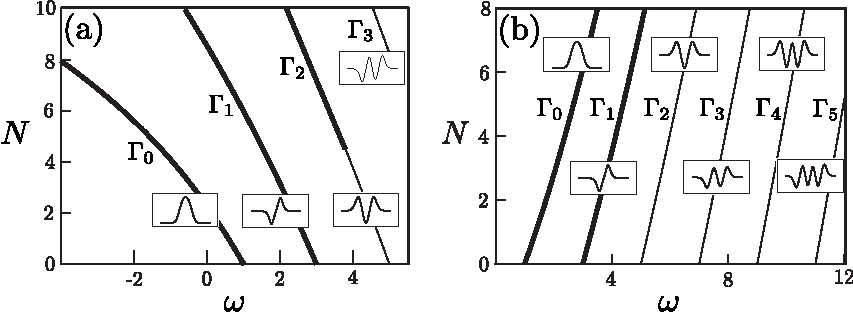
\includegraphics[scale = 1]{pic/stability for nho with constant pseudopotential}
	\caption{
		$N(\omega)$ curves for equation \eqref{eq:nho}, with (a) $\sigma_0 = 1$, (b) $\sigma_0 = -1$.
		Bold (thin) segments correspond to stable (unstable) solutions.
		Insets show schematic profiles of solutions $u_n(x)$ from each family $\Gamma_n$.
	}
\label{fig:branches-nho}
\end{figure}

Before we can move on let's briefly resume our goals in this chapter.
We study localized solutions of equation \eqref{eq:gpe-parabolic} with periodic pseudopotential \eqref{eq:gpe-parabolic-pseudopotential}.
We apply linear stability analysis to find stable solutions among them.
Our baseline model for comparison is well-studied equation \eqref{eq:nho} for nonlinear harmonic-oscillator with constant pseudopotential.
We pay special attention to the localized solutions with linear counterpart, and study how the presence of periodic pseudopotential $P(x)$ of the cosine form \eqref{eq:gpe-parabolic-pseudopotential} affects their stability.

\section{Small-Amplitude Localized Solutions with Linear Counterpart}

For Eq.~\eqref{eq:nho-periodic} let's consider a small-amplitude limit of solutions with linear counterpart.
As we say above, such solutions $u_n(x)$ originate from the bifurcation of eigenstates $(\tilde{\omega}_n, \tilde{u}_n(x))$ of harmonic-oscillator equation \eqref{eq:ho} and form families $\Gamma_n = (\omega_n, u_n(x))$.
If the amplitude of $u_n(x)$ is small the localized solutions from branch $\Gamma_n$ are approximated by expansions \cite{ZezyulinAlfimovKonotopPerecGarcia2008},
\begin{equation}
	u_n(x) = \varepsilon \tilde{u}_n(x) + o(\varepsilon), \quad \omega_n = \tilde{\omega}_n - \varepsilon^2 \Delta_n + o(\varepsilon^2),
\label{eq:small-amplitude-expansion}
\end{equation}
where $\varepsilon \ll 1$ is a small parameter, and
\begin{equation}
	\Delta_n = \int \limits_{-\infty}^{+\infty} P(x) \tilde{u}_n^4(x) dx = \dfrac{1}{2^{2n} (n!)^2 \pi} \int \limits_{-\infty}^{+\infty} P(x) H_n^4(x) e^{-2x^2} dx.
\label{eq:Delta_n}
\end{equation}

Let's address stability of these small-amplitude solutions.
We note that with the help of expansion \eqref{eq:small-amplitude-expansion}, operator $\mathcal{L}_+ \mathcal{L}_-$ in \eqref{eq:eigenvalue-problem-gpe-parabolic-analytical} may be considered as a perturbation of operator $\mathcal{L}_n^2$, where
\begin{equation}
	\mathcal{L}_n = \partial_{xx} + 2n + 1 - x^2.
\end{equation}
Specifically,
\begin{eqnarray*}
	&& \mathcal{L}_+ = \mathcal{L}_n + \varepsilon^2 (3 P(x) \tilde{u}_n^2(x) - \Delta_n) + o(\varepsilon^2); \\
	&& \mathcal{L}_- = \mathcal{L}_n + \varepsilon^2 (P(x) \tilde{u}_n^2(x) - \Delta_n) + o(\varepsilon^2).
\end{eqnarray*}
% TODO: Consider to use $\mathcal{M}_n$ instead of $M_n$.
So, for the operator $\mathcal{L}_+ \mathcal{L}_-$ we can write
\begin{equation}
	\mathcal{L}_+ \mathcal{L}_- = \mathcal{L}_n^2 + \varepsilon^2 M_n + o(\varepsilon^2),
\label{eq:perturbed-operator}
\end{equation}
where
\begin{equation}
	M_n = (2 P(x) \tilde{u}_n^2(x) - \Delta_n) \mathcal{L}_n + \mathcal{L}_n (P(x) \tilde{u}_n^2(x) - \Delta_n).
\label{eq:Mn}
\end{equation}
Operator $\mathcal{L}_n$ is self-adjoint in $L^2$ space, and its spectrum consists of eigenvalues $\varkappa_k = 2(n - k)$ with corresponding eigenfunctions $\tilde{u}_k(x)$, $k = 0, 1, \dots$  in the form \eqref{eq:ho-solutions}.
The spectrum is equidistant, all the eigenvalues being simple.
There are infinitely many negative eigenvalues, $n$ positive eigenvalues, and one zero eigenvalue.
The eigenvalues $\widetilde{\Lambda}_k$ of operator $\mathcal{L}_n^2$ are squared eigenvalues of $\mathcal{L}_n$, i.e. $\widetilde{\Lambda}_k = \varkappa_k^2 = 4 (k - n)^2$, corresponding to the same eigenfunctions $\tilde{u}_k(x)$.
This means that the spectrum of $\mathcal{L}_n^2$ includes $n$ {\it double positive eigenvalues} $\widetilde{\Lambda}_k = 4 (n - k)^2$, $k = 0, 1, \dots, (n - 1)$, one {\it simple zero eigenvalue} and {\it infinitely many simple positive eigenvalues}.
Each of the double eigenvalues has an invariant subspace spanned by two functions, $\tilde{u}_k(x)$ and $\tilde{u}_{2n - k}(x)$.
If $n = 0$, then all eigenvalues of $\mathcal{L}_n^2$ are simple.

Generically, small perturbation of $\mathcal{L}_n$ results in {\it splitting} of the double eigenvalues.
Each of them can split into (i) two real eigenvalues of the perturbed operator or (ii) two complex-conjugate eigenvalues.
If the case (i) takes place for each double eigenvalue, then small-amplitude localized solutions bifurcating form the $n$-th linear eigenstate are marginally stable, at least in some vicinity of the bifurcation.
However, if at least for one double eigenvalue the case (ii) takes place, then the bifurcating small-amplitude solutions  are unstable in vicinity of the bifurcation.

To address the splitting of double eigenvalues when passing from operator $\mathcal{L}_n^2$ to the perturbed one, $\mathcal{L}_+ \mathcal{L}_-$ in \eqref{eq:perturbed-operator}, we construct an {\it asymptotic expansion for perturbed eigenvalues} following \cite{ZezyulinAlfimovKonotopPerecGarcia2008}.
Under the actions of the perturbation, each double eigenvalue $\widetilde{\Lambda}_k$ splits into two simple ones:
\begin{equation}
	\Lambda_{k, 1} = \widetilde{\Lambda}_k + \varepsilon^2 \gamma_1 + o(\varepsilon^2), \quad \Lambda_{k, 2} = \widetilde{\Lambda}_k + \varepsilon^2 \gamma_2 + o(\varepsilon^2),
\label{eq:eigenvalues-split}
\end{equation}
where the coefficients $\gamma_{1,2}$ are the eigenvalues of the 2$\times$2 matrix
\begin{equation}
	\widetilde{M}_n =
	\begin{pmatrix}
		\langle M_n \tilde{u}_k, \tilde{u}_k \rangle & \langle M_n \tilde{u}_k, \tilde{u}_{2n - k} \rangle \\
		\langle M_n \tilde{u}_{2n - k}, \tilde{u}_k \rangle & \langle M_n \tilde{u}_{2n - k}, \tilde{u}_{2n - k} \rangle
	\end{pmatrix}.
\label{eq:M}
\end{equation}
Therefore, if the eigenvalues of $\widetilde{M}_n$ are real for each $k = 0, 1, \dots, n - 1$, then the spectrum of $\mathcal{L}_+ \mathcal{L}_-$ remains real and the nonlinear localized solution $u_n(x)$ is stable, at least for sufficiently small $\varepsilon$.
Otherwise, if eigenvalues of $\widetilde{M}_n$ are complex for some $k = 0, 1, \dots, n - 1$, then solution $u_n(x)$ is unstable in a vicinity of the bifurcation.
None that, as no double eigenvalues exist for $n = 0$, the small-amplitude solutions of the family $\Gamma_0$ are stable for any $P(x)$.

Using explicit expressions for the eigenfunctions $\tilde{u}_n(x)$ from \eqref{eq:small-amplitude-expansion} and expressions for $M_n$ from \eqref{eq:Mn}, one can compute the entries of the matrix $\widetilde{M}_n$:
\begin{align}
\langle M_n \tilde{u}_k &, \tilde{u}_k \rangle = \frac{8(n-k)}{\pi 2^{(n+k)} n! k!} \int \limits_{-\infty }^{+\infty} P(x) H_n^2(x) H_k^2(x) e^{-2 x^2} dx \notag \\ & - \frac{4(n-k)}{\pi 2^{2n}(n!)^2} \int \limits_{-\infty }^{+\infty} P(x) H_n^4(x) e^{-2 x^2} dx; \label{eq:Mn11} \\
\langle M_n \tilde{u}_k &, \tilde{u}_{2n-k} \rangle = -\langle M_n \tilde{u}_{2n-k}, \tilde{u}_k \rangle = \notag \\ & = \frac{4 (n-k)}{\pi 2^{2n} n! \sqrt{k! (2n-k)!}} \int \limits_{-\infty}^{+\infty} P(x) H_n^2(x) H_{2n-k}(x) H_k(x) e^{-2 x^2} dx;  \label{eq:Mn12} \\
\langle M_n \tilde{u}_{2n-k} &, \tilde{u}_{2n-k} \rangle = -\frac{8(n-k)}{\pi 2^{(3n-k)} n! (2n-k)!} \int \limits_{-\infty}^{+\infty} P(x) H_n^2(x) H_{2n-k}^2(x) e^{-2 x^2} dx \notag \\ & + \frac{4(n-k)}{\pi 2^{2n} (n!)^2} \int \limits_{-\infty}^{\infty} P(x) H_n^4(x) e^{-2 x^2} dx. \label{eq:Mn22}
\end{align}
Formulas \eqref{eq:Mn11} -- \eqref{eq:Mn22} with $P(x) = \pm 1$ were used in \cite{ZezyulinAlfimovKonotopPerecGarcia2008} to explore the stability of small-amplitude nonlinear solutions in the model with constant pseudopotential.

\section{Branches of Nonlinear Localized Solutions for Periodic Pseudopotential, $P(x) = P_0 + P_1 \cos (\Omega x)$}

We present our numerical and analytical results for pseudopotential of the cosine form \eqref{eq:gpe-parabolic-pseudopotential}.
It represents a sum of a constant part $P_0$ and a periodic part $P_1 \cos (\Omega x)$.
In what follow below we conclude that the relation between the magnitudes of $|P_0|$ and $|P_1|$ is important.
Hence, it's necessary to consider two cases separately: (a) $|P_0| \gtrsim |P_1|$, when the constant component is not negligible, and (b) $|P_0| \ll |P_1|$, when the constant component is negligible and pseudopotential \eqref{eq:gpe-parabolic-pseudopotential} should be treated as a function with zero mean. 
We consider each of these cases separately.

\subsection{Periodic pseudopotential with Non-Zero Mean, $|P_0| \gtrsim |P_1|$}

If $P_0$ component of pseudopotential is not negligible, one can scale out the absolute value of it, by replacing 
\begin{equation}
	\Psi \to \Psi / \sqrt{|P_0|}, \quad P_1 / |P_0| \to P_1.
\end{equation}
Equation \eqref{eq:gpe-parabolic} takes form
\begin{equation}
	i \Psi_t + \Psi_{xx} + x^2 \Psi + (\sigma_0 + P_1 \cos (\Omega x)) |\Psi|^2 \Psi = 0.
\label{eq:gpe-non-zero-mean}
\end{equation}
where $\sigma_0 \equiv P_0 / |P_0| = \mathrm{sign} (P_0)$.
Stationary states equation in this case has form
\begin{equation}
	u_{xx} + (\omega - x^2) u + (\sigma_0 + P_1 \cos (\Omega x)) u^3 = 0.
\label{eq:nho-non-zero-mean}
\end{equation}
A generic picture of localized solutions of equation \eqref{eq:nho-non-zero-mean} can be obtained by means of a numerical shooting algorithm.
A representative example of the respective $N(\omega)$ curves with $\sigma_0 = 1$, $P_1 = 2$ (which implies that the sign of the pseudopotential periodically flips), and $\Omega = 12$ is displayed in Figure~\ref{fig:branches-nho-periodic-attractive}.
One can immediately observe that, apart from branches $\Gamma_n$ originating from their linear counterparts, numerous branches of localized solutions {\it without linear counterpart} exist too.
Thus, the presence of the periodic component in the pseudopotential essentially enriches the diversity of available solutions.
This contrasts with the case of nonlinear harmonic-oscillator with constant pseudopotential, see Figure~\ref{fig:branches-nho}.
However, we did not find stable solutions without linear counterpart.
On Figure~\ref{fig:branches-nho-periodic-attractive} the only stables solutions correspond to branches $\Gamma_0$, $\Gamma_1$, $\Gamma_2$.

\begin{figure}[h]
\centering
	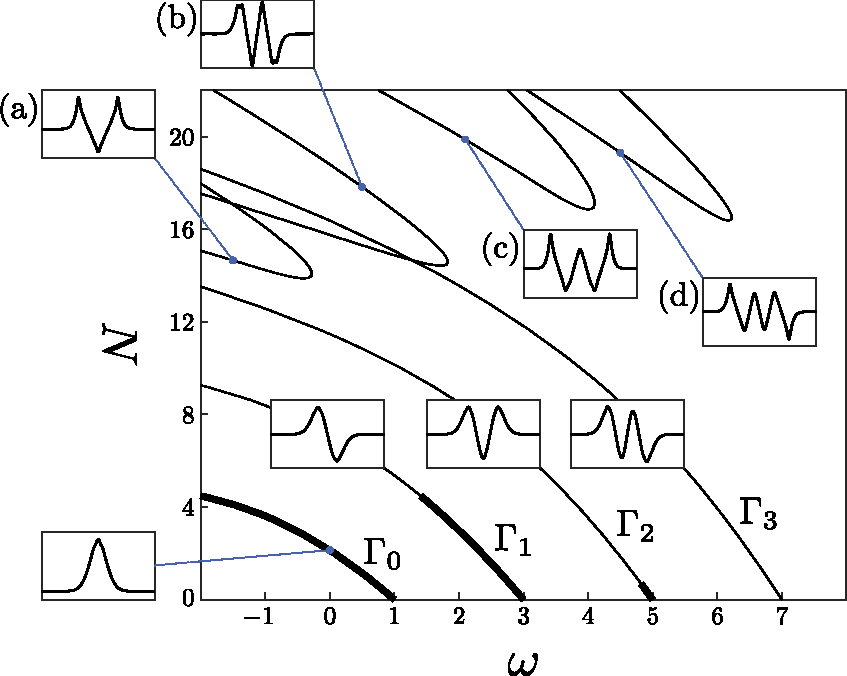
\includegraphics[scale = 1]{pic/branches for cosine nho, case (a)}
	\caption{
		Curves $N(\omega)$ of localized solution families for equation \eqref{eq:nho-non-zero-mean} with non-zero mean cosine pseudopotential with $\sigma_0 = 1$, $P_1 = 2$, and $\Omega = 12$.
		Thin and bold lines show unstable and stable solution families.
		Branches $\Gamma_n$, $n = 0, 1, 2, 3$ represent solutions with linear counterpart.
		Insets on top and outside of the branches are representative profiles $u(x)$ of solutions obtained from the corresponding families.
		Branches (a), (b), (c), and (d) represent solutions without linear counterpart.
		All of them were found to be unstable.
	}
\label{fig:branches-nho-periodic-attractive}
\end{figure}

Similar situation takes place for $\sigma_0 = -1$, while all other parameters remain the same, $P_1 = 2$ and $\Omega = 12$.
Respective $N(\omega)$ curves are presented in Figure~\ref{fig:branches-nho-periodic-repulsive}.
Localized solutions without linear counterpart correspond to branches (a) and (b).
Branches $\Gamma_0$, $\Gamma_1$ have stability regions.
All other families were found to be unstable.

\begin{figure}[h]
\centering
	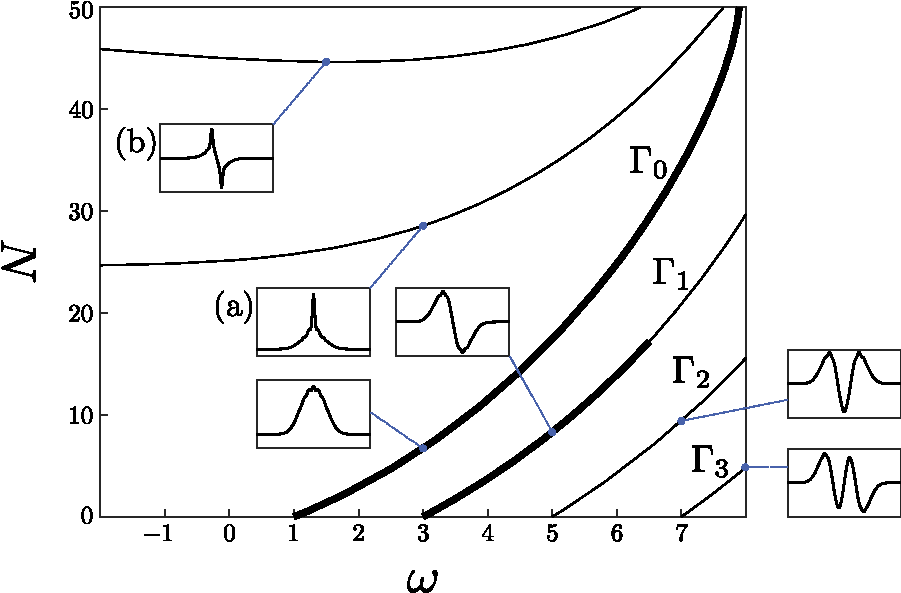
\includegraphics[scale = 1]{pic/branches for cosine nho, case (b)}
	\caption{
		Curves $N(\omega)$ of localized solution families for equation \eqref{eq:nho-non-zero-mean} with non-zero mean cosine pseudopotential with $\sigma_0 = -1$, $P_1 = 2$, and $\Omega = 12$.
		Thin and bold lines show unstable and stable solution families.
		Branches $\Gamma_n$, $n = 0, 1, 2, 3$ represent solutions with linear counterpart, two of them, $\Gamma_0$ and $\Gamma_1$, have regions of stability.
		All other families are unstable.
		Insets with blue dashed lines represent profiles $u(x)$ of the solutions.
	}
\label{fig:branches-nho-periodic-repulsive}
\end{figure}

In the limit of the rapidly oscillation of $P(x)$, $\Omega \to \infty$, localized solutions of \eqref{eq:nho-non-zero-mean} may be approximated by solutions of nonlinear harmonic-oscillator equation with constant pseudopotential \eqref{eq:nho}.
The asymptotic formula can be obtained by means of averaging with respect to fast oscillations (see, e.g. \cite{AbdullaevCaputoKraenkelMalomed}):
\begin{equation}
	u(x) = v(x) + \frac{1}{\Omega^2} \bigg( w(x) + P_1 w^3(x) \cos (\Omega x) \bigg) + o \bigg( \frac{1}{\Omega^2} \bigg), \quad \Omega \to \infty.
\label{eq:nho-non-zero-mean-asymptotic}
\end{equation}
Here $v(x)$ is a solution of Eq.~\eqref{eq:nho}, and $w(x)$ is a localized solution of the linear equation
\begin{equation}
	w_{xx} + (\omega - x^2 + 3 \sigma_0 v^2(x)) w = -\frac{3}{2} P_1^2 v^5(x).
\end{equation}
We stress that asymptotic relation \eqref{eq:nho-non-zero-mean-asymptotic} is valid for nonlinear solutions of arbitrary amplitudes (i.e. not only in the small-amplitude limit), provided that $\Omega^2$ is large enough.

\begin{figure}[h]
\centering
	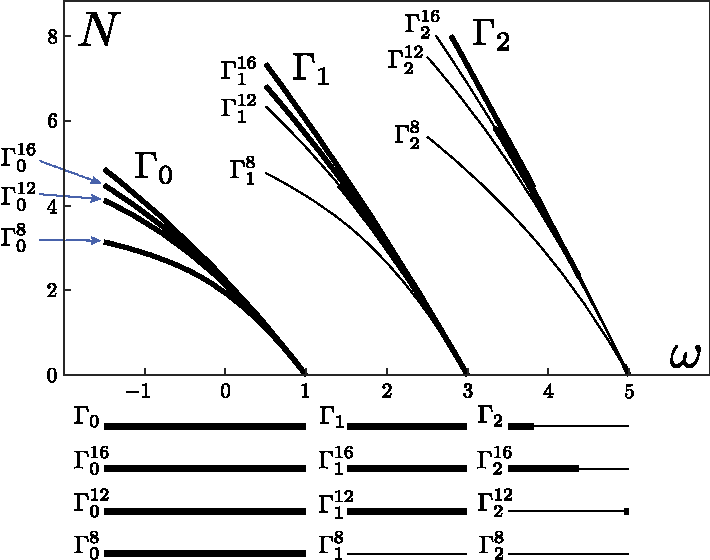
\includegraphics[scale = 1]{pic/branches with linear counterpart, non-zero mean cosine nho}
	\caption{
		Curves $N(\omega)$ of branches $\Gamma_n^{\Omega}$ for equation \eqref{eq:nho-non-zero-mean} with $\sigma_0 = 1$, $P_1 = 2$, and $\Omega = 8, 12, 16$.
		Only branches with $n = 0, 1, 2$ are shown.
		For comparison, the corresponding dependencies $\Gamma_n$ for nonlinear harmonic-oscillator \eqref{eq:nho} for the case $\sigma_0 = 1$ are show too.
		These curves are identical to those in Figure~\ref{fig:branches-nho}~(a).
		According to \eqref{eq:nho-non-zero-mean-asymptotic} branches $\Gamma_n^{\Omega}$ approaches $\Gamma_n$ as $\Omega$ grows.
		Bold (thin) lines correspond to stable (unstable) solutions.
		For convenience the stability of the families $\Gamma_n^{\Omega}$ and $\Gamma_n$ is duplicated by straight lines under the main plot.
	}
\label{fig:branches-with-linear-counterpart-non-zero-mean}
\end{figure}

Figure~\ref{fig:branches-with-linear-counterpart-non-zero-mean} shows the branches $\Gamma_0$, $\Gamma_1$, and $\Gamma_2$ for different spatial frequencies of the periodic pseudopotential, $\Omega = 8$, $\Omega = 12$, and $\Omega = 16$.
For convenience in Figure~\ref{fig:branches-with-linear-counterpart-non-zero-mean} we use the following notation.
We denote $\Gamma_n$ branches of equation \eqref{eq:nho} for nonlinear harmonic-oscillator with constant pseudopotential with parameter $\sigma_0 = 1$.
Branches $\Gamma_n^{\Omega}$ correspond to solutions of equation \eqref{eq:nho-non-zero-mean} with different frequencies $\Omega$ of pseudopotential.
According to the asymptotic prediction \eqref{eq:nho-non-zero-mean-asymptotic}, branches $\Gamma_n^{\Omega}$ approach the corresponding branches $\Gamma_n$ of equation \eqref{eq:nho} as $\Omega$ grows.
Additionally, Eq.~\eqref{eq:nho-non-zero-mean-asymptotic} implies that stability of a localized solution under the action of the rapidly oscillating pseudopotential is determined by stability of its counterpart in the nonlinear harmonic-oscillator model \eqref{eq:nho} with constant pseudopotential.
Indeed, the presence of eigenvalues with non-zero real parts in the perturbative spectrum of a nonlinear harmonic-oscillator solution implies the existence of such eigenvalues in the spectrum of the corresponding localized solution of \eqref{eq:nho-non-zero-mean} if $\Omega$ is large enough.
For example, the segment of the branch $\Gamma_1^8$ (obtained for parameters $\sigma_0 = 1$, $P_1 = 2$, $\Omega = 8$) shown in Figure~\ref{fig:branches-with-linear-counterpart-non-zero-mean} is completely unstable, but stability of the corresponding family for $n = 1$ restores for higher values of $\Omega$, which agrees with nonlinear harmonic-oscillator limit, where this branch is entirely stable.
For the branch $\Gamma_2$ the situation is more complex.
Small-amplitude solutions belonging to $\Gamma_2^8$ are unstable, but they become stable for $\Gamma_2^{12}$.
However, Eq.~\eqref{eq:nho-non-zero-mean-asymptotic} implies that the further increase of $\Omega$ will necessarily leads to the destabilization of these solutions (see branch $\Gamma_2^{16}$), because in the nonlinear harmonic-oscillator limit the small amplitude solutions belonging to $\Gamma_2$ are unstable.
% The possibility to manage the stability of small-amplitude nonlinear localized solutions by tuning frequency of the periodic component of the pseudopotential has been reported in \cite{KevrekidisFrantzeskakis}.

To check predictions of the linear-stability analysis, we have performed simulations of the evolutions of localized solutions in the framework of time-dependent GPE \eqref{eq:gpe-non-zero-mean}, using an implicit finite-difference scheme from \cite{TrofimovPeskov} that has been already used in Chapter~\ref{chapter:III}.
In the simulation, solutions which are predicted to be linearly stable keep their shape indefinitely long, see Figure~\ref{fig:stability-nho-non-zero-mean}~(e).
Solutions that are predicted to be unstable typically transform into a pulsating object localized over one period of the pseudopotential, see Figure~\ref{fig:stability-nho-non-zero-mean}~(f).

\begin{figure}[h]
\centering
	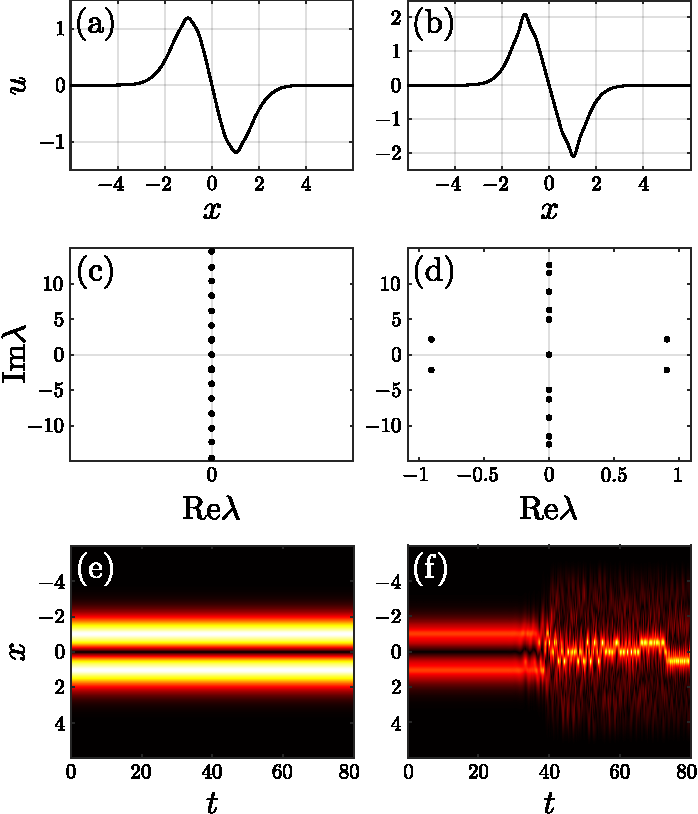
\includegraphics[scale = 1]{pic/stability, non-zero mean cosine nho}
	\caption{
		Results of stability analysis for solutions belonging to the branch $\Gamma_1$ of \eqref{eq:gpe-non-zero-mean} with pseudopotential $P(x) = 1 + 2 \cos (12 x)$, and different parameters of $\omega$.
		Shapes $u(x)$ of the stationary solutions are presented in panels (a) $\omega = 2$ and (b) $\omega = 0$.
		The linear-stability spectrums are in panels (c) and (d) correspondingly.
		The evolutionary simulations are presented in panels (e) and (f).
		Localized solution with parameter $\omega = 2$ is stable, while solutions with parameter $\omega = 0$ is unstable.
	}
\label{fig:stability-nho-non-zero-mean}
\end{figure}

\subsection{Periodic pseudopotential with Zero Mean, $|P_0| \ll |P_1|$}

According to the results of the previous section, the effect of a rapidly oscillating pseudopotential with non-zero mean may be approximated using the standard nonlinear harmonic-oscillator model with uniform nonlinearity.
However, the situation becomes essentially different for the case $|P_0| \ll |P_1|$.
If $P_0$ component of the pseudopotential can be neglected, we drop $P_0$, and rescale equation \eqref{eq:gpe-parabolic} by replacing
\begin{equation}
	\Psi \to \Psi / \sqrt{|P_1|},
\end{equation}
which leads to the equation
\begin{equation}
	i \Psi_t + \Psi_{xx} + x^2 \Psi + \sigma_1 \cos (\Omega x) |\Psi|^2 \Psi = 0,
\label{eq:gpe-zero-mean}
\end{equation}
where $\sigma_1 = P_1 / |P_1| = \mathrm{sign}(P_1)$.
Stationary states equation has the form
\begin{equation}
	u_{xx} + (\omega - x^2) u + \sigma_1 \cos (\Omega x) u^3 = 0.
\label{eq:nho-zero-mean}
\end{equation}
The $N(\omega)$ curves for \eqref{eq:nho-zero-mean} with $\sigma_1 = $ and $\Omega = 8$ are shown in Figure~\ref{fig:stability-nho-zero-mean}.
Here we again observe the branches $\Gamma_n$ bifurcating from the linear limit and various families without linear counterparts, see branches (a), (b), (b'), (c), (d) in Figure~\ref{fig:stability-nho-zero-mean}.
The branches $\Gamma_n$ feature stable and unstable segments.
Most part of the localized solutions without linear counterpart being unstable, however we found one branch  without linear counterpart, family (b) on the corresponding inset of Figure~\ref{fig:stability-nho-zero-mean}, that features small stability region.

\begin{figure}[h]
\centering
	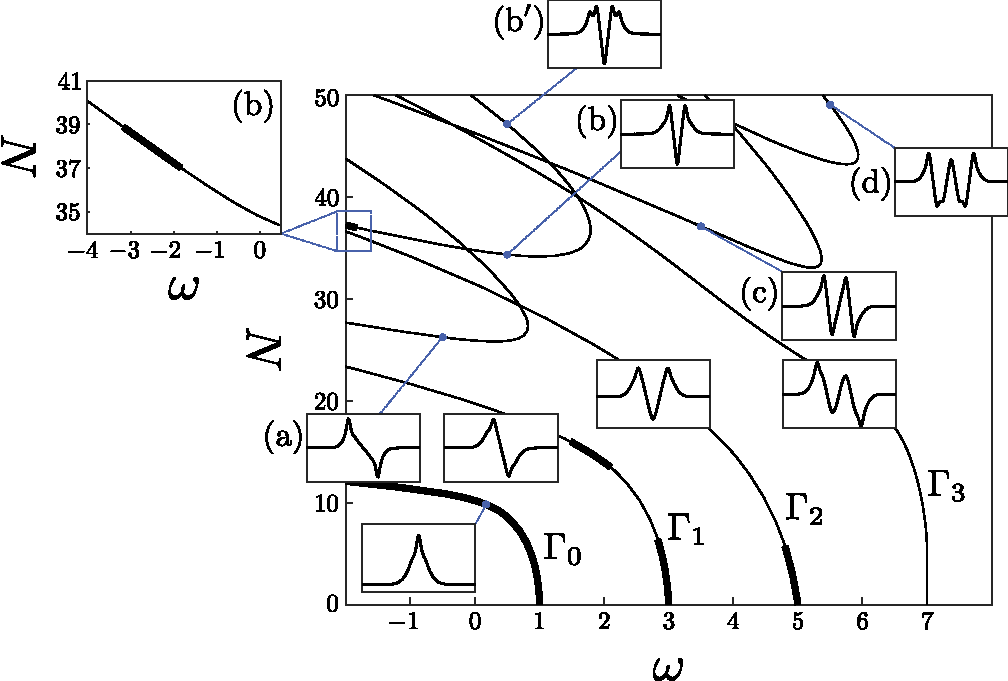
\includegraphics[scale = 1]{pic/branches for cosine nho, zero mean}
	\caption{
		Curves $N(\omega)$ for localized solutions of equation \eqref{eq:nho-zero-mean} with parameters $\sigma_1 = 1$ and $\Omega = 8$.
		Thin and bold lines show unstable and stable solution families.
		Insets depicts profiles of the solutions.
		Additional window in the upper left corner shows stability region for solutions from the branch (b) without linear counterpart.
	}
\label{fig:stability-nho-zero-mean}
\end{figure}

Let's focus on the localized solutions with linear counterpart under action of rapidly oscillating pseudopotential.
In the limit $N \\ 1$, weakly nonlinear solutions belonging to branches $\Gamma_n$, $n = 0, 1, \dots$, are produced by equations \eqref{eq:small-amplitude-expansion} where $\Delta_n$ is given by \eqref{eq:Delta_n}, with $P(x) = \sigma_1 \cos (\Omega x)$.
The numerical found values of $\Delta_n$, $n = 0, 1, 2$ for $\sigma_1$ and several different values of $\Omega$ are presented in Table~\ref{tab:Delta_n}.
\begin{table}[tbp]
\centering
\begin{tabular}{ccccc}
\hline
	$\Omega$ & \, 0 \, & \, 2 \, & \, 8 \, & \, 18 \\ \hline
	$n = 0$ & \, $3.9894 \cdot 10^{-1}$ \, & \, $2.4197 \cdot 10^{-1}$ \, & \, $1.3383 \cdot 10^{-4}$ \, & \, $1 \cdot 10^{-18}$ \\
	$n = 1$ & \, $2.9921 \cdot 10^{-1}$ \, & \, $-1.2100 \cdot 10^{-1}$ & $5.4536 \cdot 10^{-3} $ \, & \, $2 \cdot 10^{-15}$ \\
	$n = 2$ & \, $2.5557 \cdot 10^{-1}$ \, & \, $-1.3611 \cdot 10^{-1}$ \, & \, $2.1097 \cdot 10^{-2} $ \, & \, $5 \cdot 10^{-13}$ \\ \hline
\end{tabular}
\caption{
	The values of $\Delta _{n}$, $n = 0, 1, 2$, calculated as per Eq.~\eqref{eq:Delta_n} for $P(x) = \cos \left( \Omega x \right)$, $\Omega = 0, 2, 8, 18$.
	They determine the perturbative shift of chemical potential of weakly nonlinear localized solutions, pursuant to Eq.~\eqref{eq:small-amplitude-expansion}.
}
\label{tab:Delta_n}
\end{table}

To find the asymptotic form of $\Delta_n$ for $\Omega \to \infty$, we note that, for any arbitrary polynomial of degree $2m$
\begin{equation}
	Q_{2m}(x) = a_{2m} x^{2m} + a_{2m - 1} x^{2m - 1} + \dots + a_0,
\end{equation}
the following asymptotic relation holds
\begin{equation}
	\int \limits_{-\infty}^{+\infty} Q_{2m}(x) e^{-2 x^2} \cos (\Omega x)~dx \approx (-1)^m \frac{a_{2m} \sqrt{2 \pi} \Omega^{2m}}{2^{4m + 1}} e^{-\Omega^2 / 8}, \quad \Omega \to \infty.
\label{eq:polynomial-asymptotic}
\end{equation}
Since the coefficient in front of the highest-power term in the Hermite polynomial $H_n(x)$ is $2^n$, equation \eqref{eq:polynomial-asymptotic} with $Q_{2m}(x)$ substituted by  $H_n(x)$ yields
\begin{equation}
	\Delta_n \approx \frac{\sqrt{2} \Omega^{4n}}{2^{6n + 1} (n!)^2 \sqrt{\pi}} e^{-\Omega^2 / 8}, \quad \Omega \to \infty.
\label{eq:Delta_n-asymptotic}
\end{equation}
Therefore, for sufficiently large $\Omega$, $\Delta_n$ are all positive and decay exponentially, which agrees with the data in Table~\ref{tab:Delta_n}.

In the small-amplitude limit, the stability of localized solutions with linear counterpart is determined by the eigenvalues of matrix $\widetilde{M}_n$, see \eqref{eq:M}.
One can compute these eigenvalues numerically with any necessary accuracy.
The results for tow different values of frequency, $\Omega = 8$ and $\Omega = 16$, are summarized in Tables~\ref{tab:M-eigenvalues-8} and \ref{tab:M-eigenvalues-16}.
In these tables, $n$ is the index of the branch $\Gamma_n$.
For instance, $n = 2$ means that the brach $\Gamma_2$, which starts from $\tilde{\omega}_2 = 2 \cdot 2 + 1 = 5$, is under consideration.
While $k$, running from $0$ to $n - 1$, enumerates double eigenvalues $\widetilde{\Lambda}_k = 4(n - k)^2$.
Each cell with $n > k$ contains either tow real numbers or symbol ``$\mathbb{C}$''.
These number are real eigenvalues of matrix $\widetilde{M}_n$, whereas symbol ``$\mathbb{C}$'' indicates that eigenvalues of $\widetilde{M}_n$ are complex, and the corresponding low-amplitude solutions of the branch $\Gamma_n$ are unstable.
For $n < k$ the double eigenvalues do not exist (marked with dashes at the corresponding positions in the tables).

\begin{table}[tbp]
\centering
\begin{tabular}{cccccc}
\hline
	& \, $n = 1$ \, & \, $n = 2$ \, & \, $n = 3$ \, & \, $n = 4$ \, & \, $n = 5$ \\ \hline
	$k = 0$ & \, $\begin{array}{c} 0.132 \\ -0.028 \end{array}$ \, & \, $\begin{array}{c} -0.012 \\ 0.203 \end{array}$ \, & \, $\mathbb{C}$ \, & \, $\begin{array}{c} 0.424 \\ -0.828 \end{array}$ \, & \, $\begin{array}{c} -0.845 \\ -0.660 \end{array}$ \\ \hline
	$k = 1$ & \, $-$ \, & \, $\begin{array}{c} -0.176 \\ 0.159 \end{array}$ \, & \, $\begin{array}{c} 0.432 \\ -0.190 \end{array}$ \, & \, $\begin{array}{c} -0.486 \\ 0.048 \end{array}$ \, & \, $\begin{array}{c} 0.356 \\ 0.944 \end{array}$ \\ \hline
	$k = 2$ & \, $-$ \, & \, $-$ \, & \, $\begin{array}{c} -0.068 \\ -0.132 \end{array}$ \, & \, $\begin{array}{c} -0.206 \\ 0.196 \end{array}$ \, & \, $\begin{array}{c} 0.531 \\ -0.600 \end{array}$ \\ \hline
	$k = 3$ & \, $-$ \, & \, $-$ \, & \, $-$ \, & \, $\mathbb{C}$ \, & \, $\begin{array}{c} 0.166 \\ -0.122 \end{array}$ \\ \hline
	$k = 4$ & \, $-$ \, & \, $-$ \, & \, $-$ \, & \, $-$ \, & \, $\mathbb{C}$ \\ \hline
\end{tabular}
\caption{
	Eigenvalues of matrix $\widetilde{M}_n$ in the case $P(x) = \cos (8x)$.
	Here $n$ is the index of branch $\Gamma_n$, and $k$ enumerates double eigenvalues $\widetilde{\Lambda}_k = 4(n - k)^2$.
	Each cell with $n > k$ contains either tow real numbers or symbol ``$\mathbb{C}$''.
	These number are real eigenvalues of matrix $\widetilde{M}_n$, whereas symbol ``$\mathbb{C}$'' indicates that eigenvalues of $\widetilde{M}_n$ are complex, and the corresponding low-amplitude solutions of the branch $\Gamma_n$ are unstable.
	Results in this table agree with Figure~\ref{fig:stability-nho-zero-mean}.
}
\label{tab:M-eigenvalues-8}
\end{table}

% TODO: Check the values in the table. Possible there is mistake, $\Omega = 18$, not $16$.
\begin{table}[tbp]
\centering
\begin{tabular}{cccccc}
\hline
	& $n = 1$ & $n = 2$ & $n = 3$ & $n = 4$ & $n = 5$ \\ \hline
	$k = 0$ & $\begin{array}{c} -2.0 \cdot 10^{-11} \\ 5.7 \cdot 10^{-10} \end{array}$ & $\begin{array}{c} -7.6 \cdot 10^{-9} \\ -9.2 \cdot 10^{-7} \end{array}$ & $\begin{array}{c} -8.7 \cdot 10^{-7} \\ 2.2 \cdot 10^{-4} \end{array}$ & $\begin{array}{c} -4.0 \cdot 10^{-5} \\ -1.2 \cdot 10^{-2} \end{array}$ & $\begin{array}{c} -9.5 \cdot 10^{-4} \\ 1.5 \cdot 10^{-1} \end{array}$ \\ \hline
	$k = 1$ & $-$ & $\begin{array}{c} -4.2 \cdot 10^{-9} \\ 7.3 \cdot 10^{-8} \end{array}$ & $\begin{array}{c} -5.8 \cdot 10^{-7} \\ -3.6 \cdot 10^{-5} \end{array}$ & $\begin{array}{c} -3.0 \cdot 10^{-5} \\ 3.3 \cdot 10^{-3} \end{array}$ & $\begin{array}{c} -7.6 \cdot 10^{-4} \\ -6.8 \cdot 10^{-2} \end{array}$ \\ \hline
	$k = 2$ & $-$ & $-$ & $\begin{array}{c} -3.4 \cdot 10^{-7} \\ 3.9 \cdot 10^{-6} \end{array}$ & $\begin{array}{c} -2.0 \cdot 10^{-5} \\ -6.8 \cdot 10^{-4} \end{array}$ & $\begin{array}{c} -5.7 \cdot 10^{-4} \\ 2.6 \cdot 10^{-2} \end{array}$ \\ \hline
	$k = 3$ & $-$ & $-$ & $-$ & $\begin{array}{c} -1.3 \cdot 10^{-5} \\ 1.0 \cdot 10^{-4} \end{array}$ & $\begin{array}{c} -3.6 \cdot 10^{-4} \\ -6.8 \cdot 10^{-3} \end{array}$ \\ \hline
	$k = 4$ & $-$ & $-$ & $-$ & $-$ & $\begin{array}{c} -2.7 \cdot 10^{-4} \\ 1.5 \cdot 10^{-3} \end{array}$ \\ \hline
\end{tabular}
\caption{
	Eigenvalues of matrix $\widetilde{M}_n$ for $P(x) = \cos (16 x)$.
	The same notation as for Table~\ref{tab:M-eigenvalues-8} is used.
}
\label{tab:M-eigenvalues-16}
\end{table}

To be specific, let us describe in details the branch $\Gamma_2$ in the case of $P(x) = \cos (8x)$, Table~\ref{tab:M-eigenvalues-8}.
In this case, there are tow double eigenvalues in the spectrum, $\widetilde{\Lambda}_0 = 16$ and $\widetilde{\Lambda}_1 = 4$.
According to Table~\ref{tab:M-eigenvalues-8} and equation \eqref{eq:eigenvalues-split}, they split as
\begin{eqnarray}
	&& \Lambda_{0, 1} = 16 - 0.012 \cdot \varepsilon^2 + \dots, \quad \Lambda_{0, 2} = 16 + 0.203 \cdot \varepsilon^2 + \dots; \\
	&& \Lambda_{1, 1} = 4 - 0.176 \cdot \varepsilon^2 + \dots, \quad \Lambda_{1, 2} = 4 + 0.159 \cdot \varepsilon^2 + \dots.
\end{eqnarray}
Hence, the small-amplitude solutions belonging to branch $\Gamma_2$ are stable in this case.
The situation is different for branches $\Gamma_{3,4,5}$ from Table~\ref{tab:M-eigenvalues-8}.
For each of these branches the bifurcation of a complex-conjugate pair occurs: for $n = 3$ the eigenvalue $\widetilde{\Lambda}_0 = 36$ splits into complex eigenvalues, while for $n = 4$ and $n = 5$ the same happens for $\widetilde{\Lambda}_2 = 4$.
Therefore, for $\Omega = 8$ the small-amplitude solutions are stable  for branches $\Gamma_{0, 1, 2}$, but unstable for $\Gamma_{3, 4, 5}$.
Table~\ref{tab:M-eigenvalues-16} is produced for $\Omega = 16$.
It implies that the small-amplitude solutions are stable for all branches $\Gamma_{1, \dots, 5}$.

To explain the different stability of small-amplitude solutions with different values of frequency $\Omega$, we consider the behaviour of the eigenvalues of $\widetilde{M}_n$ at $\Omega \to \infty$.
Using explicit results given by equations \eqref{eq:Mn11}--\eqref{eq:Mn22} and asymptotic relation \eqref{eq:Delta_n-asymptotic}, we obtain
\begin{align}
\langle M_n \tilde{u}_k, \tilde{u}_k \rangle & \sim -\frac{2\sqrt{2} (n - k) \Omega^{4n}}{2^{6n} (n!)^2 \sqrt{\pi}} e^{-\Omega^2 / 8}; \\
\langle M_n \tilde{u}_k, \tilde{u}_{2n-k} \rangle = -\langle M_n \tilde{u}_{2n-k}, \tilde{u}_k \rangle & \sim \frac{2\sqrt{2} (n - k) \Omega^{4n}}{2^{6n} n! \sqrt{k! (2n - k)!} \sqrt{\pi}} e^{-\Omega^2 / 8}; \\
\langle M_n \tilde{u}_{2n-k}, \tilde{u}_{2n-k} \rangle & \sim -\frac{4\sqrt{2} (n - k) \Omega^{2(3n - k)}}{\sqrt{\pi} 2^{3 (3n - k)} n! (2n - k)!} e^{-\Omega^2 / 8}.
\end{align}
These relations imply that
\begin{equation}
	\widetilde{M}_n =
	\begin{pmatrix}
		O(\Omega^{4n} e^{-\Omega^2 / 8}) & O(\Omega^{4n} e^{-\Omega^2 / 8}) \\
		O(\Omega^{4n} e^{-\Omega^2 / 8}) & O(\Omega^{2(3n-k)} e^{-\Omega^2 / 8})
	\end{pmatrix},
	\quad \Omega \to \infty.
\end{equation}
All elements of the matrix $\widetilde{M}_n$ are of the same order, except for the one in the right lower corner which is of greater order since $n > k$.
It mean that, for $\Omega$ large enough, eigenvalues of $\widetilde{M}_n$ are real, hence the solutions from branches $\Gamma_n$ for arbitrary $n$ are stable in the small-amplitude limit.
This explains the difference between Table~\ref{tab:M-eigenvalues-8} and Table~\ref{tab:M-eigenvalues-16}.
The increase of the frequency from $\Omega = 8$ to $\Omega = 16$ results in stabilization of some small-amplitude solutions. 

Results of our asymptotic findings are illustrated in Figure~\ref{fig:branches-with-linear-counterpart-zero-mean}, where numerically generated $N(\omega)$ curves for $\Omega = 8$, $\Omega = 12$, and $\Omega = 16$ are depicted.
It follows from these plots that the branch $\Gamma_0$ is the ``most stable'' one for all the three values of $\Omega$.
One also notice that, for the greatest value $\Omega = 16$ there exist a ``stability window'' in a vicinity of the bifurcations for all branches $\Gamma_{0,1,2,3}$, in agreement with the asymptotic results presented above.

\begin{figure}[h]
\centering
	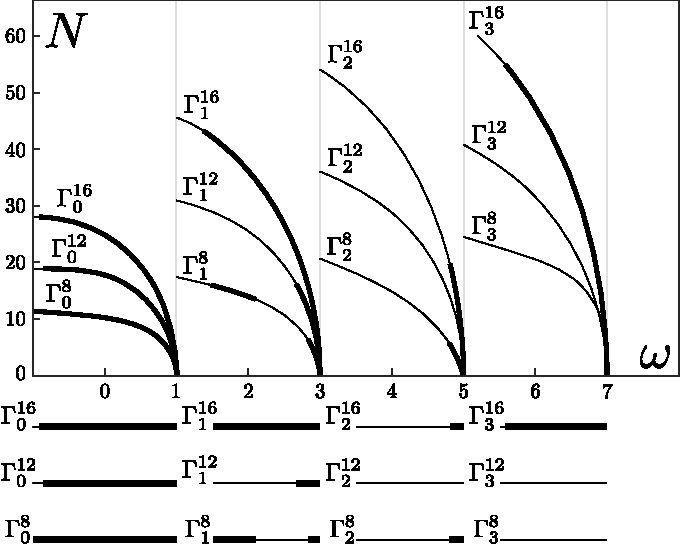
\includegraphics[scale = 1]{pic/branches with linear counterpart, zero mean cosine nho}
	\caption{
		Curves $N(\omega)$ of branches $\Gamma_n$, $n = 0, 1, 2, 3$ for equation \eqref{eq:nho-zero-mean} wi(-th $\sigma_1 = 1$ and $\Omega = 8, 12, 16$.
		The following notation is used: branch $\Gamma_n^{\Omega}$ corresponds to the branch with linear counterpart $\Gamma_n$, obtained for equation \eqref{eq:nho-zero-mean} where the frequency of pseudopotential equals $\Omega$.
		Bold (thin) lines correspond to stable (unstable) solutions.
		For convenience the stability of the families $\Gamma_n^{\Omega}$ is duplicated by straight lines under the main plot.
	}
\label{fig:branches-with-linear-counterpart-zero-mean}
\end{figure}

Numerical study of the temporal evolution of localized solutions in the framework of time-dependent GPE \eqref{eq:gpe-parabolic} confirms the prediction of the linear-stability analysis, see Figure~\ref{fig:stability-nho-zero-mean}.
As an example of a distinctive pattern of dynamical behaviour of unstable stationary solution under small perturbation, in Figure~\ref{fig:stability-nho-zero-mean} we display the transformation of an unstable solution from the branch $\Gamma_1$ into a pulsating object localized over one period of the pseudopotential $P(x) = \cos (8x)$.

\pagebreak
\begin{figure}[h]
\centering
	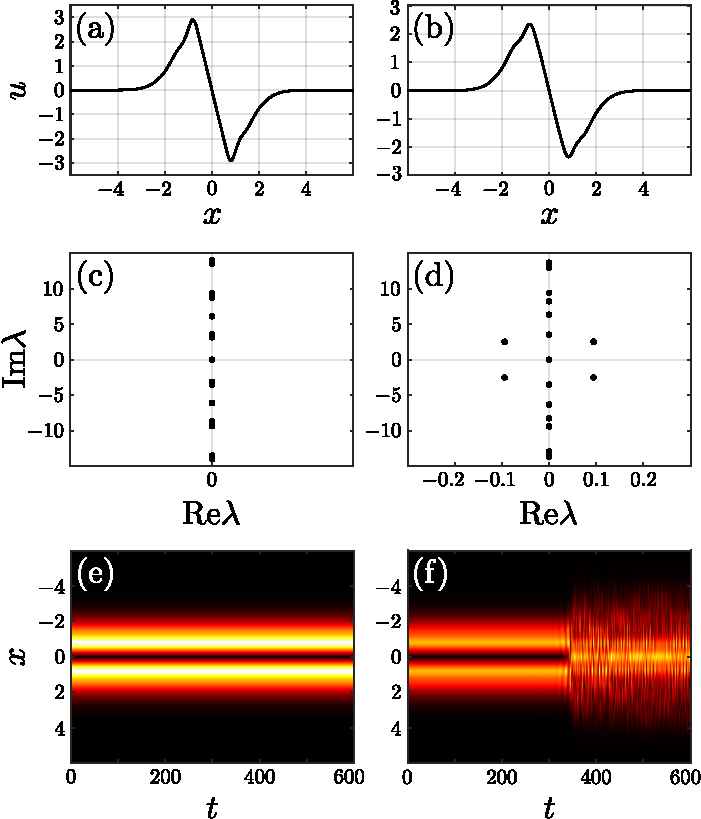
\includegraphics[scale = 1]{pic/stability, zero mean cosine nho}
	\caption{
		Results of stability analysis for solutions belonging to the branch $\Gamma_1$ of \eqref{eq:gpe-zero-mean} with pseudopotential $P(x) = \cos (8 x)$, and different parameters of $\omega$.
		Shapes $u(x)$ of the stationary solutions are presented in panels (a) $\omega = 2$ and (b) $\omega = 2.5$.
		The linear-stability spectrums are in panels (c) and (d) correspondingly.
		The evolutionary simulations are presented in panels (e) and (f).
		Localized solution with parameter $\omega = 2$ is stable, while solutions with parameter $\omega = 2.5$ is unstable.
	}
\label{fig:stability-nho-zero-mean}
\end{figure}
\pagebreak

\section{Summary}

In this chapter we studied localized stationary solutions of Gross--Pitaevskii equation with the harmonic-oscillator potential and pseudopotential $P(x)$, which is a periodic function oscillating with spatial frequency $\Omega$.
Let's summarize out results.
It was found that the presence of periodic pseudopotential significantly enrich the variety of localized solutions, in comparison with the well-studied case of the uniform nonlinearity \eqref{eq:nho}.
Specifically, GPE with periodic pseudopotential admits solutions without linear counterpart which do not exist in the case of $P(x) = \pm 1$.
As concerns solutions bifurcating from eigenstate of linear problem, their properties are essentially different depending on the presence constant additive term in $P(x)$ (non-zero mean value).
If the mean is non-zero, then properties of nonlinear solutions in a rapidly oscillating pseudopotential may be approximated using solutions for the standard nonlinear harmonic-oscillator model (with constant pseudopotential).
However, the reduction to the standard model with constant nonlinearity does not work for the system with zero-mean periodic pseudopotential.
Most interesting, in this we have found that the rapidly oscillating pseudopotential can stabilize small-amplitude localized solutions belonging to higher families, which are unstable in the model with $P(x)$ of non-zero mean.
Specifically, for any given branch with index $n$, there exists a threshold value of the spatial frequency $\Omega_n$, such that the small-amplitude solutions belonging to this branch are stable for $\Omega > \Omega_n$.
All results of our work were published in \cite{AlfimovGegelLebedevMalomedZezyulin}.


% Conclusion
% \chapter*{Conclusion}
\addcontentsline{toc}{chapter}{Conclusion}
\label{conclusion}

In the present work one-dimensional stationary states of Bose--Einstein condensate cloud were studied.
Dynamics of the condensate in so-called mean-field ap­proximation is well described by the Schr\"odinger type equation \eqref{eq:intro-gpe} with spatial non-au­tonomous terms.
One of this term, $U(x)$, corresponds to the potential that is used to confine condensate.
Another term, $P(x)$, called pseudopotential, describes the dependence of scattering length on the coordinates that can be made non-constant by various experimental techniques, such as Feshbach resonance.

In our study we focused on special subclass of the solutions, so-called stationary localized modes, SLMs, satisfying the ansatz \eqref{eq:intro-ansatz} and the localization conditions \eqref{eq:intro-localization}.
The profile of the stationary solutions is described by equation \eqref{eq:intro-stationary}.
Our goal was to identify stationary solutions for equation \eqref{eq:intro-gpe} and study their stability.
To describe stationary solutions for the case of both periodic potential and pseudopotential functions we developed a symbolic dynamics approach.
It allows under certain conditions to describe the solutions of equation \eqref{eq:intro-stationary} in terms of bi-infinite symbolic sequences, so-called codes.
Based on the structure of coding sets $\mathscr{U}_L^{\pm}$, which are the Poicar\'e map domains for equation \eqref{eq:intro-stationary}, one can assign a symbolic code to each stationary solution.
Besides, under specified conditions such correspondence is bijective.
This approach was applied to the cases of piecewise and cosine-form pseudopotential.
It turns out that there exists plethora of localized solutions in this model.
For cosine-form pseudopotential our comprehensive study revealed new types of stable solutions.

For the case of harmonic potential trap and periodic pseudopotential family of SLMs was also studied.
Since harmonic potential is not periodic, coding approach cannot be applied to such problem.
Numerical analysis showed that presence of periodic pseudopotential significantly enriches the family of localized solutions.
We also studied stability of low-amplitude localized solutions with asymptotic methods and describe the effect of the frequency of pseudopotential on their stability.
Stability of found stationary localized solutions was studied numerically with spectral method and confirmed by numerical simulation with finite-difference scheme.

Let's summarize in details main results of the thesis.
\begin{enumerate}
	\item The statements about the presence and absence of singular solutions of equation \eqref{eq:intro-stationary} are formulated and proved.
		It is shown that in the case $P(x) > 0$ all solutions of \eqref{eq:intro-stationary} are regular.
		If $P(x)$ is negative at the point $x_0$, $P(x_0) < 0$, then there exist two one-parametric families of solutions, which tend to infinity at the point $x_0$.
		In the case $Q(x) < 0$ and $P(x) < 0$, it is shown that all solutions of equation \eqref{eq:intro-stationary} are singular.
	\item An approach of one-to-one coding of solutions for equation \eqref{eq:intro-stationary} with periodic functions $Q(x)$, $P(x)$ has been developed.
		This approach requires some conditions to be met.
		These conditions are formulated in a form of two hypothesis and an efficient algorithm for their numerical verification is provided.
	\item For the case $U(x) \equiv 0$, $P(x) = A + \cos 2x$ the set of stationary localized modes for equation \eqref{eq:intro-gpe} has been studied.
		A new stable previously unknown solution, called {\it dipole soliton}, was found.
	\item In the case of harmonic potential well it was shown that including of periodic pseudopotential results in new classes of SLMs without linear counterpart.
		For the pseudopotential with zero mean, it was concluded that the increase of pseudopotential frequency stabilize low-amplitude solutions.
\end{enumerate}

In conclusion, let's also consider possible directions in which the current work can be further developed and generalized.
One of such directions is to consider a model described by GPE \eqref{eq:intro-gpe} for both periodic potential and periodic pseudopotential with different spatial frequencies.
Our coding approach can be applied to such case.
It's interesting to study family of stationary localized solutions and their stability in a view of interplay between these two spatial frequencies.

Another generalization of this study is related to two component BEC models \cite{TrippenbachGoralRzazewskiMalomedBand, OhbergSantos, SvidzinskyChui, NavarroCarreteroGonzalezKevrekidis, KevrekidisFrantzeskakis2016}.
These models describe mixtures of ultracold atoms of two different types.
It would be interesting to extend the methods developed in this work by considering four-dimensional plane of initial data and analysing counterparts of coding sets in this case. 
This study may result in classification of vector solitons admitted by the system under given parameters.
The next step of this perspective research would be the analysis of their stability.
It may be promising, since it was shown that including nonlinear lattice in one component of the two component model may stabilize two-dimensional vector solitons \cite{BorovkovaMalomedKartashov}.
Following the setup of the last paper, it would be quite interesting to extend the approach developed in this work to multidimensional problems.


\appendix
\renewcommand\thechapter{\Alph{chapter}}

\chapter{Lemma on Bounded Solutions}
\label{appendix:lemma-on-bounded-solutions}

\begin{lemma*}[On bounded solutions]
	Let $f(t, z)$ be a function that is continuous with respect to $t$ and continuously differentiable with respect to $z$.
	Let $f(t, z)$ is defined for $t \ge t_0$, $|z| < +\infty$, and have the following properties:
	\begin{itemize}
		\item[(i)] for $|z| < \rho$, $\rho > 0$, the estimate $|f(t, z)| < \eta_{\rho}(t)|z|$ is valid, where $\eta_{\rho}(t) \in L_1(t_0; +\infty)$;
		\item[(ii)] for all $z_1$, $z_2$ such that $|z_{1,2}| < \rho$, $\rho > 0$, there exists function $\tilde{\eta}_{\rho}(t) \in L_1(t_0; +\infty)$, such that $|f(t, z_2) - f(t, z_1)| \le \tilde{\eta}_{\rho}(t) |z_2 - z_1|$;
		\item[(iii)] for $|z| < \rho$, $\rho > 0$, the estimate $|f_z(t, z)| < \theta_{\rho}(t) |z|$ is valid, where $\theta_{\rho} \in L_1(t_0, +\infty)$;
		\item[(iv)] for all $z_1$, $z_2$ such that $z_{1,2} < \rho$, $\rho > 0$, there exists function $\tilde{\theta}_{\rho} \in L_1(t_0; +\infty)$, such that $|f_z(t, z_2) - f_z(t, z_1)| \le \tilde{\theta}_{\rho} |z_2 - z_1|$.
	\end{itemize}
	Then for the equation
	\begin{equation}
		z_{tt} - \alpha z_t + f(t, z) = 0, \quad \alpha > 0
		\label{eq:lemma-bs-main}
	\end{equation}
	the following statements are valid:
	\begin{itemize}
		\item[(A)] for each solution $z(t)$ of the equation \eqref{eq:lemma-bs-main} that is bounded when $t \to +\infty$ there exists $C \in \mathbb{R}$ such that $z(t) \to C$ as $t \to +\infty$;
		\item[(B)] for each $C \in \mathbb{R}$ there exists unique solution $Z(t, C)$ of the equation \eqref{eq:lemma-bs-main}, defined on a segment $(t_C; +\infty)$, such that
		\begin{equation}
			Z(t, C) = C + o(1), \quad t \to +\infty;
		\end{equation}
		\item[(C)] family of solutions $Z(t, C)$ is $C^1$-smooth with respect to the parameter $C$.
	\end{itemize}
\end{lemma*}
\begin{proof}
	Let us prove the statement (A) first.
	With the method of variation of parameters one can find that a solution of the equation \eqref{eq:lemma-bs-main} satisfies the equality:
	\begin{equation}
		z(t) = \varkappa_1 + \varkappa_2 e^{\alpha t} + \int \limits_{t_0}^{t} e^{\alpha \eta} \left( \int \limits_{\eta}^{+\infty} e^{-\alpha \xi} f(\xi, z(\xi)) d\xi \right) d\eta.
	\end{equation}
	It follows from the condition (i) that if $z(t)$ is bounded while $t \to +\infty$ then the integral
	\begin{equation}
		\int \limits_{t_0}^{+\infty} e^{\alpha \eta} \left( \int \limits_{\eta}^{+\infty} e^{-\alpha \xi} f(\xi, z(\xi)) d\xi \right) d\eta
	\end{equation}
	converges.
	Furthermore for all bounded solutions $\varkappa_2 = 0$, hence $z(t)$ tends to some constant for $t \to +\infty$.
	That proves the point (A).
	
	Move on to the point (B).
	We make a variable change $u(t) = z(t) - C$, where $C$ is an arbitrary number.
	Rewrite the equation \eqref{eq:lemma-bs-main} in the form of a system of equations
	\begin{equation}
		y_t = Ay + F(t, y),
		\label{eq:lemma-bs-system}	
	\end{equation}
	where
	\begin{equation*}
		y = \begin{pmatrix}
			u \\ v
		\end{pmatrix}, \quad
		A = \begin{pmatrix}
			0 & 1 \\
			0 & \alpha
		\end{pmatrix}, \quad
		F(t, y) = \begin{pmatrix}
			0 \\ f(t, u + C)
		\end{pmatrix}.
	\end{equation*}
	Now we apply Theorem 9.1 from \cite[Chapter XII]{Hartman} to the system \eqref{eq:lemma-bs-system}.
	It states that the system \eqref{eq:lemma-bs-system} {\it has a solution which tends to zero at infinity} \underline{if} the following conditions are satisfied:
	\begin{itemize}
		\item[(1)] function $F(t, y)$ is continuous and $||F(t, y)|| \le \lambda(t)$ for $t \in [t_0; +\infty)$, $||y|| \le \rho$, where $\lambda(t) \in L_1(t_0; +\infty)$;
		\item[(2)] for all $g(t) = col(g_1(t), g_2(t))$, $g(t) \in L_1(t_0; +\infty)$ there exists a solution $y(t) \in L_0^{\infty}(t_0; +\infty)$ of the inhomogeneous system
		\begin{equation}
			y_t = Ay + g(t);
			\label{eq:lemma-bs-hartman}
		\end{equation}
		(hereinafter by the norm $||\cdot||$ we mean the Euclidean norm in $\mathbb{R}$).
	\end{itemize}
	
	At first, by the condition (i) if $|u| \le \rho$ and $t > t_0$ relation $||f(t, u, C)|| \le \rho \eta_{\rho} (t)$ takes place, moreover $\eta_{\rho} \in L_1(t_0; +\infty)$, hence the condition (1) of the above-mentioned theorem is satisfied.
	At second, general solution of the inhomogeneous system of equations \eqref{eq:lemma-bs-hartman} can be written as:
	\begin{eqnarray}
		&& u(t) = C_2 + \int \limits_{t_0}^{t} \left( g_1(\eta) + e^{\alpha \eta} \left( C_1 - \int \limits_{+\infty}^{\eta} e^{-\alpha \xi} g_2(\xi) d\xi \right) \right) d\eta; \\
		&& v(t) = u_t(t) - g_1(t).
	\end{eqnarray}
	Since $g_{1,2}(t) \in L_1(t_0; +\infty)$ one can choose appropriate parameters $C_1$, $C_2$ in order to get a solution which tends to zero while $t \to +\infty$, so the condition (2) of the theorem is also met.
	Thereby both of the conditions for the applied theorem take place for the system \eqref{eq:lemma-bs-system}.
	That implies existence of a solution $z(t)$ of \eqref{eq:lemma-bs-main} that approaches a given constant $C$ while $t \to +\infty$ for all $C$.
	
	Now we prove the uniqueness of such solution.
	Suppose that for the same $C$ there exist two solutions $u_{1,2}(t)$ for equation
	\begin{equation}
		u_{tt} - \alpha u_t + f(t, u + C) = 0.
		\label{eq:lemma-bs-u}
	\end{equation}
	Consider their difference $\Delta(t) = u_2(t) - u_1(t)$, it satisfies the equation
	\begin{equation}
		\Delta_{tt} - \alpha \Delta_t + R(t) \Delta = 0,
		\label{eq:lemma-bs-difference}
	\end{equation}
	and a boundary condition $\Delta \to 0$ as $t \to +\infty$ takes place.
	Here
	\begin{equation}
		R(t) \equiv \dfrac{f(t, u_2(t) +C) - f(t, u_1(t) + C}{u_2(t) - u_1(t)}.
	\end{equation}
	By the condition (ii) we can apply Theorem 11 from \cite[Chapter 3]{Coppel}.
	It states that there exists a homeomorphism between the bounded solutions of the equation \eqref{eq:lemma-bs-difference} and solutions of equation
	\begin{equation}
		\Delta_{tt} - \alpha \Delta_t = 0,
	\end{equation}
	moreover (see a note to that theorem in \cite{Coppel}) this homeomorphism is a linear map.
	It means that only a zero solution of \eqref{eq:lemma-bs-difference} satisfies the zero asymptotic at infinity, i.e. $u_2(t) \equiv u_1(t)$.
	Thus we have proven the existence of the solutions family $Z(t, C)$ parametrised by $C \in \mathbb{R}$, statement (B) is proven.
	
	To prove the statement (C) one can note that the derivative
	\begin{equation}
		\dfrac{\partial Z}{\partial C}(t, C) \equiv \Theta(t, C)
	\end{equation}
	satisfies the equation \eqref{eq:lemma-bs-u} after differentiation with respect to $C$, moreover $\Theta(t, C) \to 0$ as $t \to +\infty$.
	We have
	\begin{equation}
		\Theta_{tt} - \alpha \Theta_t + f_z(t, u + C) \Theta + f_z(t, u + C) = 0.
	\end{equation}
	Here we can use Theorem 11 from \cite[Chapter 3]{Coppel} again, and using the condition (iii) we can conclude that there exists a solution of this equation $\Theta(t, C)$ such that $\Theta(t, C) \to 0$ as $t \to +\infty$, and function $\Theta(t, C)$ is continuous with respect to the parameter $C$.
	That proves the overall lemma.
\end{proof}

\chapter{Solutions of Duffing equations}
\label{appendix:solutions-of-duffing-equations}

\chapter{Strips Mapping Theorems}
\label{appendix:strips-mapping-theorems}

% TODO: Read through this carefully.
\begin{theorem}[On h-strips mapping]
\label{thm:h-strips-mapping}
	Let Poincar\'e map $\mathcal{P}$ and its inverse $\mathcal{P}^{-1}$ are defined on a complete (see Definition~\ref{def:complete-island-set}) island set $\bigcup_{i \in S} D_i$, where $S$ is a finite or countable set of indices.
	Let for all $i, j \in S$ set $V_{ji} = \mathcal{P}^{-1} (D_j) \cap D_i$ is non-empty, $\mathcal{P}$ is defined on a
	 closure $\overline{V_{ji}}$, and one of the following two conditions is met:
	\begin{enumerate}
		\item[(1)] borders $\alpha_i^{\pm}$ of an island $D_i$ are increasing curves, $\forall \vb{p} \in \overline{V_{ji}}$ signs of values $\{ a_{mn} \}$ in the matrix of the linear operator $D \mathcal{P}_{\vb{p}} = (a_{mn})$ have exactly one of the following configurations\footnote{By ``$+$'' and ``$-$'' sign we mean \underline{strict} inequalities $a_{mn} > 0$, $a_{mn} < 0$ to be held.}:
			\begin{center}
				(a) $\begin{psm} + & + \\ + & + \end{psm}$, \quad
				(b) $\begin{psm} - & - \\ - & - \end{psm}$, \quad
				(c) $\begin{psm} + & + \\ - & - \end{psm}$, \quad
				(d) $\begin{psm} - & - \\ + & + \end{psm}$;
			\end{center}
			and at the same time borders $\alpha_j^{\pm}$ of $D_j$ are increasing curves for cases (a), (b), and decreasing curves for (c), (d);
		\item[(2)] borders $\alpha_i^{\pm}$ of an island $D_i$ are decreasing curves, $\forall \vb{p} \in \overline{V_{ji}}$ signs of values $\{ a_{mn} \}$ in the matrix of the linear operator $D \mathcal{P}_{\vb{p}} = (a_{mn})$ have exactly one of the following configurations:
			\begin{center}
				(a) $\begin{psm} + & - \\ - & + \end{psm}$, \quad
				(b) $\begin{psm} - & + \\ + & - \end{psm}$,	\quad
				(c) $\begin{psm} + & - \\ + & - \end{psm}$, \quad
				(d) $\begin{psm} - & + \\ - & + \end{psm}$;		
			\end{center}
			and at the same time borders $\alpha_j^{\pm}$ of $D_j$ are decreasing curves for cases (a), (b), and increasing for (c), (d);
	\end{enumerate}
	and moreover $\exists \mu > 1$ such that $\forall p \in \overline{V_{ji}}$, $|a_{11}| \ge \mu$, then for any \emph{h}-strip $H \in D_i$, $\mathcal{P} (H) \cap D_j = \widetilde{H}_j$ is also an \emph{h}-strip, and $d_{\mathrm{h}}(\widetilde{H}_j) \le (1 / \mu) d_{\mathrm{h}}(H)$ (here $d_{\mathrm{h}}(\cdot)$ is an \emph{h}-strip thickness in a sence of Definition~\ref{def:h-thickness}).
\end{theorem}
\begin{proof}
	Let's fix indices $i, j$ and prove the theorem for a pair of islands $D_i$, $D_j$.
	Mostly we consider the case (1а).
	Other cases 
	The rest of the cases must be treated in a completely analogous way.
	Denote by $\mathbf{e}_1$, $\mathbf{e}_2$ basis vectors
	\begin{equation}
		\mathbf{e}_1 = \begin{pmatrix} 1 \\ 0 \end{pmatrix}; \quad \mathbf{e}_2 = \begin{pmatrix} 0 \\ 1 \end{pmatrix}.
	\end{equation}
	Define the following set of {\it cones}:
	\begin{align*}
		\mathbb{R}_{++}^2 = \{ \mathbf{v} \, | \, \mathbf{v} = x \mathbf{e}_1 + y \mathbf{e}_2, \; x > 0, y > 0 \}; \\
		\overline{\mathbb{R}}_{++}^2 = \{ \mathbf{v} \, | \, \mathbf{v} = x \mathbf{e}_1 + y \mathbf{e}_2, \; x \ge 0, y \ge 0 \}; \\
		\mathbb{R}_{+-}^2 = \{ \mathbf{v} \, | \, \mathbf{v} = x \mathbf{e}_1 + y \mathbf{e}_2, \; x > 0, y < 0 \}; \\
		\overline{\mathbb{R}}_{+-}^2 = \{ \mathbf{v} \, | \, \mathbf{v} = x \mathbf{e}_1 + y \mathbf{e}_2, \; x \ge 0, y \le 0 \}; \\
		\mathbb{R}_{-+}^2 = \{ \mathbf{v} \, | \, \mathbf{v} = x \mathbf{e}_1 + y \mathbf{e}_2, \; x < 0, y > 0 \}; \\
		\overline{\mathbb{R}}_{-+}^2 = \{ \mathbf{v} \, | \, \mathbf{v} = x \mathbf{e}_1 + y \mathbf{e}_2, \; x \le 0, y \ge 0 \}; \\
		\mathbb{R}_{--}^2 = \{ \mathbf{v} \, | \, \mathbf{v} = x \mathbf{e}_1 + y \mathbf{e}_2, \; x < 0, y < 0 \}; \\
		\overline{\mathbb{R}}_{--}^2 = \{ \mathbf{v} \, | \, \mathbf{v} = x \mathbf{e}_1 + y \mathbf{e}_2, \; x \le 0, y \le 0 \}. \\
	\end{align*}
	As a \underline{first} step in the proof, we show that values signs in the matrix of linear operator $D \mathcal{P}_{\vb{p}} = ( a_{mn} )$ uniquely determine the structure of cones mapping in each point $\vb{p}$ of the set $\overline{V_{ji}}$.
	For the case (a) we have:
	\begin{equation*}
	\forall \mathbf{v} = \begin{pmatrix} x \\ y \end{pmatrix} \in \overline{\mathbb{R}}_{++}^2, \ D \mathcal{P}_{\vb{p}}(\mathbf{v}) = \begin{pmatrix} a_{11} & a_{12} \\ a_{21} & a_{22} \end{pmatrix} \begin{pmatrix} x \\ y \end{pmatrix} = \begin{pmatrix} \widetilde{x} > 0 \\ \widetilde{y} > 0\end{pmatrix} \in \mathbb{R}_{++}^2.	
	\end{equation*}
	It is easy to check that the complete scheme of the cones mapping for the case (1) of the theorem looks as follows:
	\begin{eqnarray*}
		(\textup{a}) & D \mathcal{P}_{\vb{p}} (\overline{\mathbb{R}}_{++}^2) \in \mathbb{R}_{++}^2, \quad D \mathcal{P}_{\vb{p}} (\overline{\mathbb{R}}_{--}^2) \in \mathbb{R}_{--}^2; \\
		(\textup{b}) & D \mathcal{P}_{\vb{p}} (\overline{\mathbb{R}}_{++}^2) \in \mathbb{R}_{--}^2, \quad D \mathcal{P}_{\vb{p}} (\overline{\mathbb{R}}_{--}^2) \in \mathbb{R}_{++}^2; \\
		(\textup{c}) & D \mathcal{P}_{\vb{p}} (\overline{\mathbb{R}}_{++}^2) \in \mathbb{R}_{+-}^2, \quad D \mathcal{P}_{\vb{p}} (\overline{\mathbb{R}}_{--}^2) \in \mathbb{R}_{-+}^2; \\
		(\textup{d}) & D \mathcal{P}_{\vb{p}} (\overline{\mathbb{R}}_{++}^2) \in \mathbb{R}_{-+}^2, \quad D \mathcal{P}_{\vb{p}} (\overline{\mathbb{R}}_{--}^2) \in \mathbb{R}_{+-}^2.
	\end{eqnarray*}
	Complete scheme for the case (2) have the following form correspondingly:
	\begin{eqnarray*}
		(\textup{a}) & D \mathcal{P}_{\vb{p}} (\overline{\mathbb{R}}_{-+}^2) \in \mathbb{R}_{-+}^2, \quad D \mathcal{P}_{\vb{p}} (\overline{\mathbb{R}}_{+-}^2) \in \mathbb{R}_{+-}^2; \\
		(\textup{b}) & D \mathcal{P}_{\vb{p}} (\overline{\mathbb{R}}_{-+}^2) \in \mathbb{R}_{+-}^2, \quad D \mathcal{P}_{\vb{p}} (\overline{\mathbb{R}}_{+-}^2) \in \mathbb{R}_{-+}^2; \\
		(\textup{c}) & D \mathcal{P}_{\vb{p}} (\overline{\mathbb{R}}_{-+}^2) \in \mathbb{R}_{--}^2, \quad D \mathcal{P}_{\vb{p}} (\overline{\mathbb{R}}_{+-}^2) \in \mathbb{R}_{++}^2; \\
		(\textup{d}) & D \mathcal{P}_{\vb{p}} (\overline{\mathbb{R}}_{-+}^2) \in \mathbb{R}_{++}^2, \quad D \mathcal{P}_{\vb{p}} (\overline{\mathbb{R}}_{+-}^2) \in \mathbb{R}_{--}^2.
	\end{eqnarray*}
	
	As a \underline{second} step we show that such cones mapping preserve in some way Lipschitz constraints and monotonicity properties for curves from $\overline{V_{ji}}$ under the $\mathcal{P}$ mapping.
	Show that for the case (1a).
	For that first of all we note that from compactness of $\overline{V_{ji}}$ the existence of the following supremum follows:
	\begin{equation*}
		\widetilde{\gamma}_{ji} = \sup \dfrac{y}{x}, \ \begin{pmatrix} x \\ y \end{pmatrix} = D \mathcal{P}_{\vb{p}} (\mathbf{v}), \ \vb{p} \in \overline{V_{ji}}, \ \mathbf{v} \in \overline{\mathbb{R}}_{++}^2.
	\end{equation*}
	Further, let there be two tow different points $\vb{p}_1 \, \vb{p}_2 \in \overline{V_{ji}}$, $\vb{p}_1 = (\psi_1, \psi_1')$, $\vb{p}_2 = (\psi_2, \psi_2')$, and besides $\psi_2 \ge \psi_1$, $\psi_2' \ge \psi_2$.
	Let points $\vb{q}_1$, $\vb{q}_2$ be the $\mathcal{P}$-images of the points $\vb{p}_1$, $\vb{p}_2$ correspondingly, $\mathcal{P}(\vb{p}_1) = \vb{q}_1 = (\phi_1, \phi_1')$, $\mathcal{P}(\vb{p}_2) = \vb{q}_2 = (\phi_2, \phi_2')$.
	Let $D \mathcal{P}_{\vb{p}_1}$ is a linearization of $\mathcal{P}$ at the point $\vb{p}_1$.
	Then the following expansion is valid:
	\begin{equation}
		\vb{q}_2 = \mathcal{P}(\vb{p}_2) = \vb{q}_1 + D \mathcal{P}_{\vb{p}_1} (\vb{p}_2 - \vb{p}_1) + r(||\vb{p}_2 - \vb{p}_1||),
	\end{equation}
	where $r(||\vb{p}_2 - \vb{p}_1||) / ||\vb{p}_2 - \vb{p}_1|| \to 0$ as $||\vb{p}_2 - \vb{p}_1|| \to 0$ (here $|||\cdot||$ is a Euclidean norm).
	Vector $\vb{p}_{\Delta} = \vb{p}_2 - \vb{p}_1 \in \overline{\mathbb{R}}_{++}^2$ which means that for its mapping by linearized operator we have $D \mathcal{P}_{\vb{p}_1} (\mathbf{p}_{\Delta}) = \mathbf{q}_{\Delta} \in \mathbb{R}_{++}^2$, and
	\begin{equation}
		\vb{q}_2 - \vb{q}_1 = \mathbf{q}_{\Delta} + r(||\vb{p}_2 - \vb{p}_1||).
	\end{equation}
	Expression above means that for ``close enough'' points $\vb{p}_1$, $\vb{p}_2$ their images satisfy the relationship $\vb{q}_2 - \vb{q}_1 \in \mathbb{R}_{++}^2$, i.e. $\phi_2 > \phi_1$, $\phi_2' > \phi_1'$.
	Moreover one can choose a value $\gamma_{ji} > \widetilde{\gamma_{ji}}$ such that the following inequality is held:
	\begin{equation}
		0 < \phi_2' - \phi_1' < \gamma_{ji} (\phi_2 - \phi_1).
	\label{eq:ordering}
	\end{equation}
	This ordering is transitive, i.e. from the relation \eqref{eq:ordering} and the second analogous relation for ``close enough'' point $\vb{p}_2$, $\vb{p}_3$,
	\begin{equation}
		0 < \phi_3' - \phi_2' < \gamma_{ji} (\phi_3 - \phi_2),
	\end{equation}
	follow the analogous relation for the points $\vb{p}_1$, $\vb{p}_3$ as well.
	That allows to spread the relation \eqref{eq:ordering} over all points $\vb{p}_1, \, \vb{p}_2 \in \overline{V_{ji}}$ that satisfies the conditions $\psi_2 \ge \psi_1$, $\psi_2' \ge \psi_1'$.
	Other cases (1b)-(1d), (2a)-(2d) can be considered in a similar way.
	
	Thus for the case (1) for all points $\vb{p}_1, \, \vb{p}_2 \in \overline{V_{ji}}$, which coordinates satisfy the relations $\psi_2 \ge \psi_1$, $\psi_2' \ge \psi_1'$, coordinates of their $\mathcal{P}$-images $\vb{q}_1 = (\phi_1, \phi_1'), \, \vb{q}_2~=~(\phi_2, \phi_2')$ depending on sings of values in matrix of $D \mathcal{P}_{\vb{p}}$, $\vb{p} \in \overline{V_{ji}}$, met exactly one of the following inequalities ($\exists \gamma_{ji}$):
	\begin{subequations}
	\begin{eqnarray}
		(\textup{a}) & 0 < \phi_2' - \phi_1' < \gamma_{ji} (\phi_2 - \phi_1); \label{eq:ordering_1a} \\
		(\textup{b}) & 0 < \phi_1' - \phi_2' < \gamma_{ji} (\phi_1 - \phi_2); \label{eq:ordering_1b} \\
		(\textup{c}) & 0 < \phi_1' - \phi_2' < \gamma_{ji} (\phi_2 - \phi_1); \label{eq:ordering_1c} \\
		(\textup{d}) & 0 < \phi_2' - \phi_1' < \gamma_{ji} (\phi_1 - \phi_2). \label{eq:ordering_1d}
	\end{eqnarray}
	\end{subequations}
	For the case (2) in its turn we have that for all points $\vb{p}_1, \, \vb{p}_2 \in \overline{V_{ji}}$, which coordinates satisfy the relations $\psi_2 \le \psi_1$, $\psi_2' \ge \psi_1'$, exactly one of the following inequalities is met:
	\begin{subequations}
	\begin{eqnarray}
		(\textup{a}) & 0 < \phi_2' - \phi_1' < \gamma_{ji} (\phi_1 - \phi_2); \label{eq:ordering_2a} \\
		(\textup{b}) & 0 < \phi_1' - \phi_2' < \gamma_{ji} (\phi_2 - \phi_1); \label{eq:ordering_2b} \\
		(\textup{c}) & 0 < \phi_1' - \phi_2' < \gamma_{ji} (\phi_1 - \phi_2); \label{eq:ordering_2c} \\
		(\textup{d}) & 0 < \phi_2' - \phi_1' < \gamma_{ji} (\phi_2 - \phi_1). \label{eq:ordering_2d}
	\end{eqnarray}
	\end{subequations}
	
	A a \underline{third} step we demonstrate how these inequalities above allow to conclude that for any h-strip $H \in D_i$ its image $\mathcal{P} H \cap D_j = \widetilde{H}_j$ is also an h-strip.
	Let an h-strip $H \in D_i$ is placed between two monotonic h-curves $\widetilde{\alpha}_i^{\pm}$.
	Endpoints of the $\widetilde{\alpha}_i^{\pm}$ belong to the boundaries $\beta_i^{\pm}$ of island $D_i$, so the $H$ is a curvilinear quadrangle bounded by curves $\widetilde{\alpha}_i^{\pm}$ and segments of curves $\beta_i^{\pm}$.
	For the case (1a) of the theorem curves $\widetilde{\alpha}_i^{\pm}$  are increasing.
	Let's consider an image of the curve $\widetilde{\alpha}_i^+$.
	According to the definition of a complete island set $\mathcal{P} (\widetilde{\alpha}_i^+)$ cross each of the boundaries $\beta_j^{\pm}$ of island $D_j$ at least once.
	At the same time $\mathcal{P} (\widetilde{\alpha}_i^+)$ cannot cross boundaries $\alpha_j^{\pm}$ because they consist of points which tends to infinity under action of $\mathcal{P}^{-1}$.
	
	Let $\mathcal{P} (\widetilde{\alpha}_i^+)$ cross one of the boundaries $\beta_j^{\pm}$ of the island $D_j$ twice.
	Denote those intersection points by $\vb{q}_1 = \mathcal{P}(\vb{p}_1), \, \vb{q}_2 = \mathcal{P}(\vb{p}_2)$.
	For the case (1a) boundaries $\alpha_j^{\pm}$ are increasing curves, and $\beta_j^{\pm}$ are decreasing, hence the points $\vb{q}_1, \, \vb{q}_2$ belong to a decreasing curve.
	From the other side points $\vb{p}_1, \, \vb{p}_2 \in \overline{V_{ji}}$ belong to increasing curve $\widetilde{\alpha}_i^+$, and hence for their $\mathcal{P}$-image coordinates $\vb{q}_1 = (\phi_1, \phi_1'), \, \vb{q}_2 = (\phi_2, \phi_2')$ inequality \eqref{eq:ordering_1a} must be held.
	This inequality means that points $\vb{q}_1, \, \vb{q}_2$ cannot belong to a decreasing curve, and $\mathcal{P} (\widetilde{\alpha}_i^+)$ cross each boundary $\beta_j^{\pm}$ only once.
	Similar statement is valid also for the $\mathcal{P} (\widetilde{\alpha}_i^-)$.
	% TODO: Add a remark on Lipschitz conditions here.
	Thereby $\mathcal{P} (\widetilde{\alpha}_i^{\pm}) \cap D_j$ are monotonic curves.
	Their type of monotonicity coincide with the monotonicity type of corresponding boundaries of the island $D_j$, moreover these curves bound the set $\mathcal{P} H \cap D_j$, hence $\mathcal{P} H \cap D_j = \widetilde{H}_j$ is an h-strip.
	Other cases can be considered in a similar way using the corresponding inequalities \eqref{eq:ordering_1b} -- \eqref{eq:ordering_1d}, \eqref{eq:ordering_2a} -- \eqref{eq:ordering_2d}.
	
	Finally, in a \underline{fourth} step of this proof we show that under the introduced constrain on $|a_{11}|$ value of linearized operator, for all h-strip $H \in D_i$, $\rho (\widetilde{H}_j) \le \mu \rho(H)$, so that thickness of an h-strip $\mathcal{P}$-image within island $D_j$ is less than thickness of an original h-strip inside island $D_i$.
	To prove that first assume that h-strips $H$ and $\widetilde{H}_j$ are well-measured in a sense on Definition~\ref{def:well-measurable-h-strip}.
	Let the thickness of the h-strip $\widetilde{H}_j$ can be measured along the vertical curve connecting points $\vb{q}_1 = (\phi_1, \phi_1'), \, \vb{q}_2 = (\phi_2, \phi_2')$, $\phi_1' < \phi_2'$.
	Consider a parametrization of that curve $\vb{q}(t) = (0, \phi'(t))$, where
	\begin{equation}
		\phi'(t) = t \phi_2' + (1 - t) \phi_1', \quad 0 \le t \le 1.
	\end{equation}
	Strip $\widetilde{H}_j$ is well-measurable, so the curve $\vb{q}(t)$ entirely belongs to $\widetilde{H}_j$.
	Since $\widetilde{H}_j = \mathcal{P} H \cap D_j$ there exists a pre-image $\vb{p}(t) = \mathcal{P}^{-1} (\vb{q}(t)) = (\psi(t), \psi'(t))$, $\vb{p}(t) \subset H$ and $\vb{q}(t) = \mathcal{P} (\vb{p}(t))$.
	For the case (1a) let's demonstrate that $\vb{p}(t)$ is a decreasing curve connecting point from the opposite boundaries $\widetilde{\alpha}_i^{\pm}$ of the strip $H$ inside $D_i$.
	Remark, here by ``decreasing'' we mean that the curve is a graph of decreasing function in $(u, u')$ coordinates, not as a function of $t$.
	The curve $\vb{q}(t)$ belongs to some set which is a $\mathcal{P}$-image of a part of the set $\overline{V_{ji}}$.
	The signs of values in the matrix of $D \mathcal{P}_{\vb{p}}$, $\vb{p} \in \overline{V_{ji}}$ have the form $\begin{psm} + & + \\ + & + \end{psm}$, so the signs of values for the linearized inverse map $D \mathcal{P}^{-1}_{\vb{q}}$ have a configuration $\begin{psm} + & - \\ - & + \end{psm}$ on the curve $\vb{q}(t)$.
	This allows to conclude the corresponding cones mapping:
	\begin{equation}
		D \mathcal{P}^{-1}_{\vb{q}(t)} (\overline{\mathbb{R}}_{-+}^2) \in \mathbb{R}_{-+}^2, \quad D \mathcal{P}^{-1}_{\vb{q}(t)} (\overline{\mathbb{R}}_{+-}^2) \in \mathbb{R}_{+-}^2.
	\label{eq:cones-backward}
	\end{equation}
	Therefore the corresponding monotonicity property \eqref{eq:ordering_2a} takes place.
	It immediately follows from \eqref{eq:ordering_2a} that the vertical curve $\vb{q}(t)$ is mapped to the decreasing curve $\vb{p}(t)$ (decreasing in $(u, u')$ coordinates).
	Moreover the inequality $\phi_1' < \phi_2'$ provides that $\psi'(t) > 0$.
	
	% TODO: Consider to color left strip as well (for all three pictures).
	\begin{figure}[h]
	\centering
		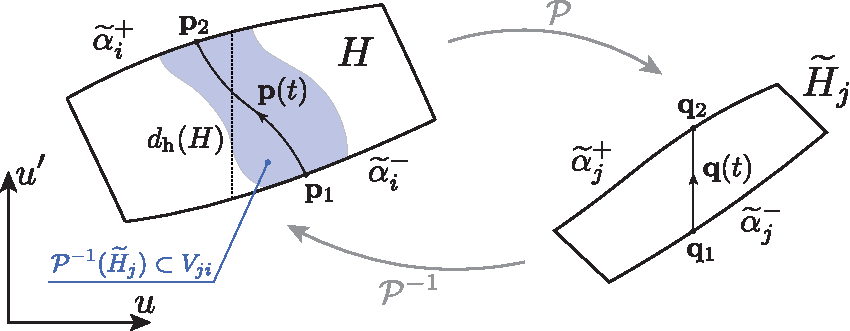
\includegraphics[scale = 1]{pic/thickness of h-strip (a)}
		\caption{
			Illustration for the proof of the h-strips thickness decrease for the case when both h-strips $H$ and $\widetilde{H}_j$ and well-measurable.
			Thickness of $H$ is measured along the vertical dotted line, thickness of $\widetilde{H}_j$ is measured along the vertical line $\vb{q}(t)$.
			Arrows indicate curves traverse directions while $t$ changes from $0$ to $1$.
			Pre-image of $\widetilde{H}_j$ strip is colored with gray.
		}
	\label{fig:thickness-of-h-strip-a}
	\end{figure}
	
	Consider tangent vectors to $\vb{p}(t)$ and $\vb{q}(t)$ (upper dot means the derivative with respect to $t$):
	\begin{eqnarray}
		&& \dot{\vb{p}}(t) = (\dot{\psi}(t), \dot{\psi}'(t)); \\
		&& \dot{\vb{q}}(t) = (0, \dot{\phi}'(t)).
	\end{eqnarray}
	In each point $t$ they are connected by the $D \mathcal{P}_{\vb{p}(t)}$ operator
	\begin{equation}
		\dot{\vb{q}}(t) = D \mathcal{P}_{\vb{p}(t)} (\dot{\vb{p}}(t)).
	\end{equation}
	Rewrite this relation in a matrix form:
	\begin{equation}
		\begin{pmatrix}
			a_{11}(t) & a_{12}(t) \\ a_{21}(t) & a_{22}(t)
		\end{pmatrix}
		\begin{pmatrix}
			\dot{\psi}(t) \\
			\dot{\psi}'(t)
		\end{pmatrix} =
		\begin{pmatrix}
			0 \\ \dot{\phi}'(t)
		\end{pmatrix}.
	\end{equation}
	% TODO: Give a cite, from where follows this fact for Poincar\'e map.
	We take into account that matrix $(a_{mn})$ is a linearization of Poincar\'e map to conclude that its determinant $a_{11}(t) a_{22}(t) - a_{12}(t) a_{21}(t) = 1$ in each point $t$.
	From the relations above and the theorem condition on values of $a_{11}(t)$ follows
	\begin{equation}
		\dot{\phi}'(t) = \dfrac{1}{a_{11}(t)} \dot{\psi}'(t) \le \dfrac{1}{\mu} \dot{\psi}'(t).
	\label{eq:to-integrate}
	\end{equation}
	Integration of \eqref{eq:to-integrate} with limits $0 \le t \le 1$ gives:
	\begin{equation}
		d_{\mathrm{h}}(\widetilde{H}_j) = \phi_2' - \phi_1' = \int \limits_0^1 \dot{\phi}'(t) dt \le \dfrac{1}{\mu} \int \limits_0^1 \dot{\psi}'(t) dt = \dfrac{1}{\mu} (\psi_2' - \psi_1').
	\label{eq:thickness-of-strip-final}
	\end{equation}
	Curve $\vb{p}(t)$ is decreasing and boundaries of $H$ are increasing curves, so it follows from general geometric considerations that $\psi_2' - \psi_1' \le d_{\mathrm{h}}(H)$, i.e. $d_{\mathrm{h}}(\widetilde{H}_j) \le (1 / \mu) d_{\mathrm{h}}(H)$.
	That gives the final statement of the theorem for well-measurable strips.
	
	\begin{figure}[h]
	\centering
		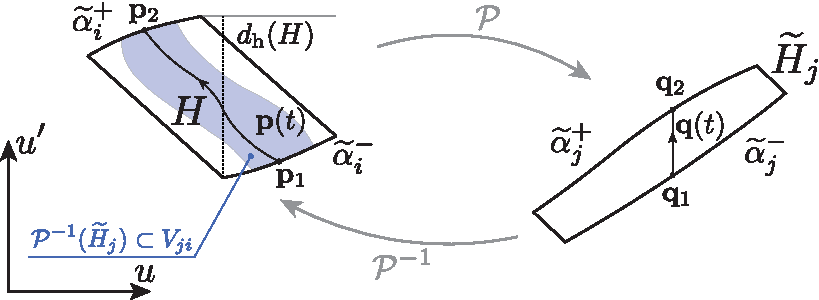
\includegraphics[scale = 1]{pic/thickness of h-strip (b)}
		\caption{
			Illustration for the proof of the h-strips thickness decrease for the case when strip $H$ is not well-measurable.
			Its thickness is measured along the vertical dotted line.
			One endpoint of that line does not belong to the strip boundary $\widetilde{\alpha}_i^+$.
			Pre-image of $\widetilde{H}_j$ strip is colored with gray.
		}
	\label{fig:thickness-of-h-strip-b}
	\end{figure}
	
	The proof above can be easily generalized to the cases when h-strips  $H$ and $\widetilde{H}_j$ are not well-measurable.
	If strip $H$ is not well-measurable, the inequality $\psi_2' - \psi_1' \le d_{\mathrm{h}}(H)$ in \eqref{eq:thickness-of-strip-final} takes place anyway.
	This fact is illustrated on Figure~\ref{fig:thickness-of-h-strip-b}.
	Vertical distance between points $\vb{p}_1, \, \vb{p}_2$ turns out to be certainly less than the width of $H$ strip.
	
	In the case when h-strip $\widetilde{H}_j$ is not well-measurable, one should choose corner points $\vb{q}_1, \, \vb{q}_2$ in a such way that the vertical distance between them equals the thickness of $\widetilde{H}_j$, and then connect $\vb{q}_1, \, \vb{q}_2$ with a monotonic decreasing curve $\vb{q}(t)$, see Fig.~\ref{fig:thickness-of-h-strip-c}.
	This is always possible due to the geometric properties of not well-measurable h-strip.
	According to the choice of points $\vb{q}_1, \, \vb{q}_2$, $d_{\mathrm{h}}(\widetilde{H}_j) = \phi_2 - \phi_1$, and all the steps above remain valid since the corresponding cones mapping with all the consequences can be also applied for the decreasing curves $\vb{p}(t)$ and $\vb{q}(t)$.
	\begin{figure}[h]
	\centering
		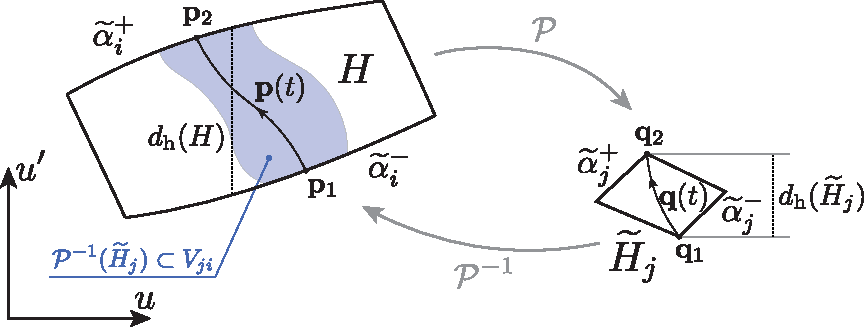
\includegraphics[scale = 1]{pic/thickness of h-strip (c)}
		\caption{
			Illustration for the proof of the h-strips thickness decrease for the case when strip $\widetilde{H}_j$ is not well-measurable.
			Thickness of $H$ and $\widetilde{H}_j$ are measured along the dotted lines.
			Pre-image of $\widetilde{H}_j$ strip is colored with gray.
	  }
	\label{fig:thickness-of-h-strip-c}
	\end{figure}
	
	If both h-strips $H$ and $\widetilde{H}_j$ are not well-measurable then two above mentioned technics should be combined together.
	During the consideration of all other cases of the theorem only type of curves monotonicity is changed, but the overall approach remains the same and can be applied with just minor adjustments.
	Theorem is proven.
\end{proof}

\pagebreak

\begin{theorem}[On v-strips mapping]
\label{thm:v-strips-mapping}
	Let Poincar\'e map $\mathcal{P}$ and its inverse $\mathcal{P}^{-1}$ are defined on a complete (see Definition~\ref{def:complete-island-set}) island set $\bigcup_{i \in S} D_i$, where $S$ is a finite or countable set of indices.
	Let for all $i, j \in S$ set $H_{ij} = \mathcal{P} (D_i) \cap D_j$ is non-empty, $\mathcal{P}^{-1}$ is defined on a
	 closure $\overline{H_{ij}}$, and one of the following two conditions is met:
	\begin{enumerate}
		\item[(1)] borders $\beta_j^{\pm}$ of an island $D_j$ are increasing curves, $\forall \vb{q} \in \overline{H_{ij}}$ signs of values $\{ b_{mn} \}$ in the matrix of the linear operator $D \mathcal{P}_{\vb{q}}^{-1} = (b_{mn})$ have exactly one of the following configurations:
			\begin{center}
				(a) $\begin{psm} + & + \\ + & + \end{psm}$, \quad
				(b) $\begin{psm} - & - \\ - & - \end{psm}$, \quad
				(c) $\begin{psm} + & + \\ - & - \end{psm}$, \quad
				(d) $\begin{psm} - & - \\ + & + \end{psm}$;
			\end{center}
			and at the same time borders $\beta_i^{\pm}$ of $D_i$ are increasing curves for cases (a), (b), and decreasing curves for (c), (d);
		\item[(2)] borders $\beta_j^{\pm}$ of an island $D_j$ are decreasing curves, $\forall \vb{q} \in \overline{H	_{ij}}$ signs of values $\{ b_{mn} \}$ in the matrix of the linear operator $D \mathcal{P}_{\vb{q}}^{-1} = (b_{mn})$ have exactly one of the following configurations:
			\begin{center}
				(a) $\begin{psm} + & - \\ - & + \end{psm}$, \quad
				(b) $\begin{psm} - & + \\ + & - \end{psm}$,	\quad
				(c) $\begin{psm} + & - \\ + & - \end{psm}$, \quad
				(d) $\begin{psm} - & + \\ - & + \end{psm}$;		
			\end{center}
			and at the same time borders $\beta_i^{\pm}$ of $D_i$ are decreasing curves for cases (a), (b), and increasing for (c), (d);
	\end{enumerate}
	and moreover $\exists \nu > 1$ such that $\forall q \in \overline{H_{ij}}$, $|b_{22}| \ge \nu$, then for any \emph{v}-strip $V \in D_j$, $\mathcal{P}^{-1} (V) \cap D_i = \widetilde{V}_i$ is also a \emph{v}-strip, and $d_{\mathrm{v}} (\widetilde{V}_i) \le (1 / \nu) d_{\mathrm{v}} (V)$ (here $d_{\mathrm{v}}(\cdot)$ is an \emph{v}-strip thickness in a sence of Definition~\ref{def:v-thickness}).
\end{theorem}
\begin{proof}
	Completely analogous to the proof of the h-strips mapping theorem.
\end{proof}

% Bibliography
\printbibliography[heading=bibintoc]

\end{document}

